\documentclass[12pt,oneside,a4paper]{article}

\usepackage{./custom}

\usepackage[light, frenchstyle,narrowiints,partialup]{kpfonts}
\usepackage{tcolorbox}
\tcbuselibrary{breakable}
\tcbuselibrary{documentation}
\usepackage{booktabs}
\usepackage{mathtools}
\usepackage{xcolor}
\usepackage[backend=biber]{biblatex}
\addbibresource{./literature.bib}

\definecolor{colback}{HTML}{ffffff}
\definecolor{subtitle}{HTML}{c5d5cb}
\definecolor{colbacktitle}{HTML}{e3e0cf}
\definecolor{colframe}{HTML}{9fa8a3}

\hypersetup{
  colorlinks=true,        % false: boxed links; true: colored links
  linkcolor=black,        % color of internal links
  citecolor=trueblue,     % color of links to bibliography
  filecolor=trueblue,     % color of file links
  urlcolor=trueblue       % color of external links
}

\newtcolorbox{mybox}[2][]{
	title=\textsc{#2},
	colback = colback,
	colbacktitle = colbacktitle,
	coltitle = gray!25!black,
	colframe = colframe,
	boxrule = .6pt, 
	subtitle style={boxrule = .1pt,colback = subtitle},
	breakable,
	sharp corners,
	enhanced,
	attach boxed title to top center={yshift=-2mm},
	#1,
}

\begin{document}
% title (fold)
\begin{titlepage}
\begin{center}

% Upper part of the page. The '~' is needed because \\
% only works if a paragraph has started.


\includegraphics[scale=0.5]{./img/dauphine_logo} \\[1.5cm]

% \textsc{\LARGE \textsc{CentraleSupélec}}\\[1.5cm]


\vfill
% Title
\rule{\textwidth}{1.6pt}\vspace*{-\baselineskip}\vspace*{2pt} % Thick horizontal line
\rule{\textwidth}{0.4pt}\\[\baselineskip] % Thin horizontal line
{ \huge  \textsc{Synthèse} \\[0.4cm]
\textsc{Microéconomie} }
\rule{\textwidth}{0.4pt}\vspace*{-\baselineskip}\vspace{3.2pt} % Thin horizontal line
\rule{\textwidth}{1.6pt}\\[1.5cm] % Thick horizontal line

\vfill
\paragraph{Foreword}
Any error or contribution should be reported
in the form of an issue, or a pull request for those
who can use \texttt{git} and \LaTeX, to
\begin{center}
  \url{https://github.com/mbataillou/Summaries/tree/master/Dauphine/Micro}
\end{center}
You can notice that there is always place for improvement
and your help is therefore welcome.
\vspace{\baselineskip}

\vfill
% Author
{\large
\begin{center}
  % \adfast{1}  \hspace{0.5cm}\textsc{\textbf{Encadrant du projet}}\hspace{0.5cm}   \adfast{1}  \\[0.3cm] \large
  {\Large  \hspace{0.5cm} \textbf{Auteurs} \hspace{0.5cm}   } \\[0.3cm]
  % \adfast{1}  \hspace{0.5cm}\textsc{Nom des élèves} \hspace{0.5cm}   \adfast{1} \\[0.3cm] \large
	\textsc{Bataillou Almagro} Marc \\
	  ---
\end{center}
}
\vfill

% Bottom of the page
{\large \today}

\end{center}
\end{titlepage}
% title (end)

\vspace{3cm}

{\tableofcontents}

\newpage


\part{Teoría} % (fold)
\label{prt:teoría_}

% part teoría_ (end)
\question{Cómo puedes determinar el valor de la resistencia al corte sin drenaje ($C_u$) de una arcilla a partir de un ensayo de compresión simple ? ¿ Qué fiabilidad te merece el resultado ?}{
	\begin{figure}[H]
			\centering
			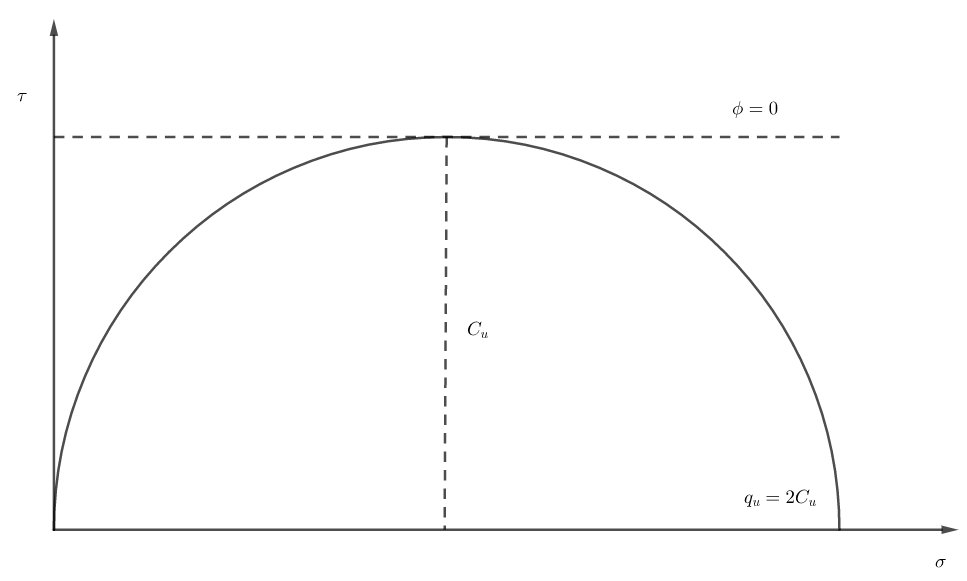
\includegraphics[width=0.5\textwidth]{img/cu}
			\caption{Circulo de Mohr: compresión simple sin drenaje}
			\label{fig:cu}
	\end{figure}
	Se rompen distintas provetas y se encuentra la envolvente de rotura. La fiabilidad del resultado dependerá del la alteración de la muestra.
}

\question{Cúando se utilizan los resultados del ensayo del molinete (vane-test) para estimar el valor de $C_u$ de una arcilla, se suele aplicar un factor de corrección que depende del índice de plasticidad del suelo. ¿ A qué se debe la necesidad de esta corrección? ¿ A partir de qué datos se ha determinado dicho factor?}{
	Se aplica por:
	\begin{itemize}
		\item Anisotropia del terreno
		\item Velocidad de cargo (más rapida que en campo)
	\end{itemize}
	Aplicamos un factor de corrección que varia en función del indice de plasticidad (IP), véase Figure~\ref{fig:mu}
	\begin{figure}[H]
			\centering
			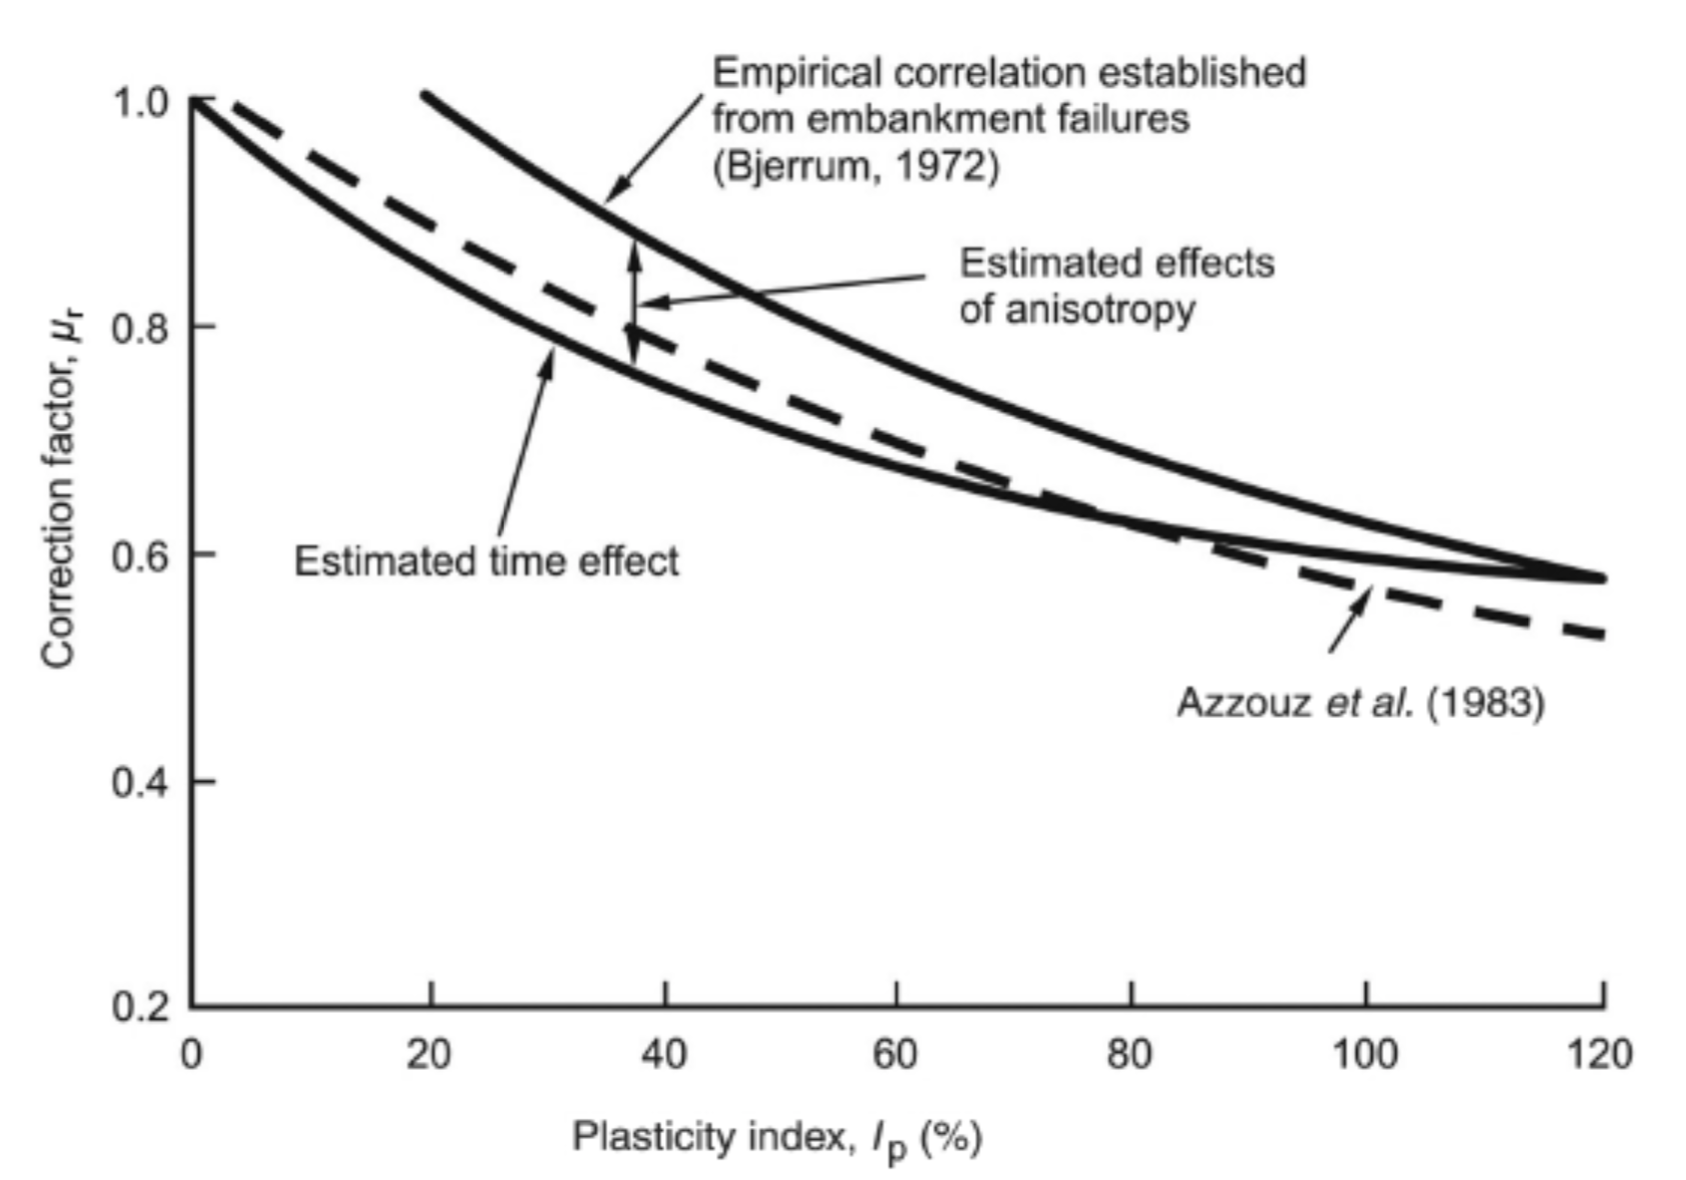
\includegraphics[width=0.5\textwidth]{img/mu}
			\caption{Factor de corrección Vane test}
			\label{fig:mu}
	\end{figure}
}

\question{Suponiendo que una arcilla se comporta con un modelo eláso-perfectamento plástico, dibujar la evolución de la presión intersticial que se medirá en un ensayo presiométrico (se considera condiciones no drenadas).}{
	\begin{figure}[H]
			\centering
			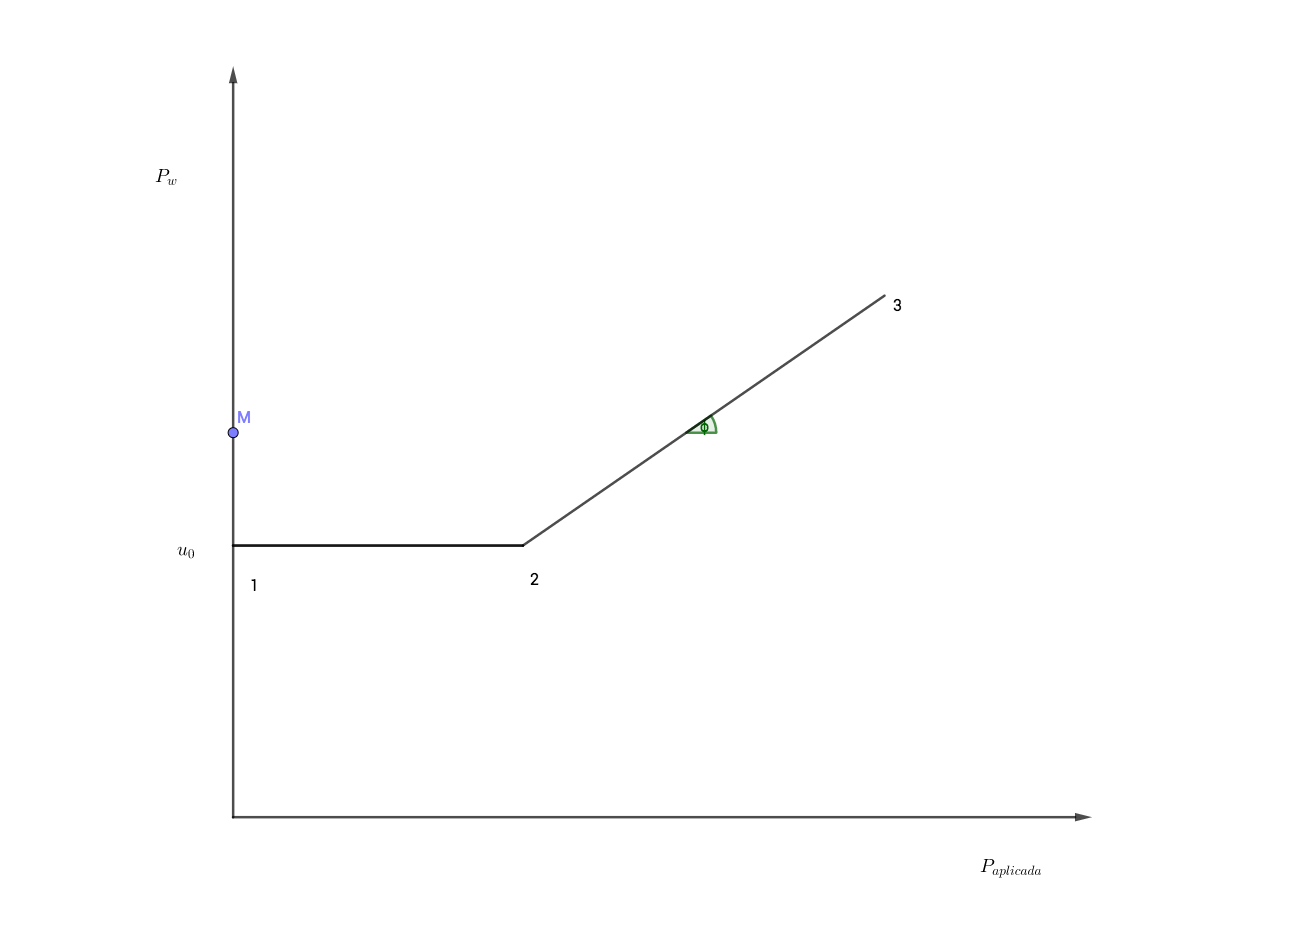
\includegraphics[width=0.5\textwidth]{img/u_evolution}
			\caption{Evolución de la presión intersticial}
			\label{fig:mu}
	\end{figure}
	Véase la evolución de los circulos de mohr en las Figure~\ref{fig:presio1},\ref{fig:presio2},\ref{fig:presio3}

	\begin{minipage}{0.5\linewidth}
		\begin{figure}[H]
		\centering
		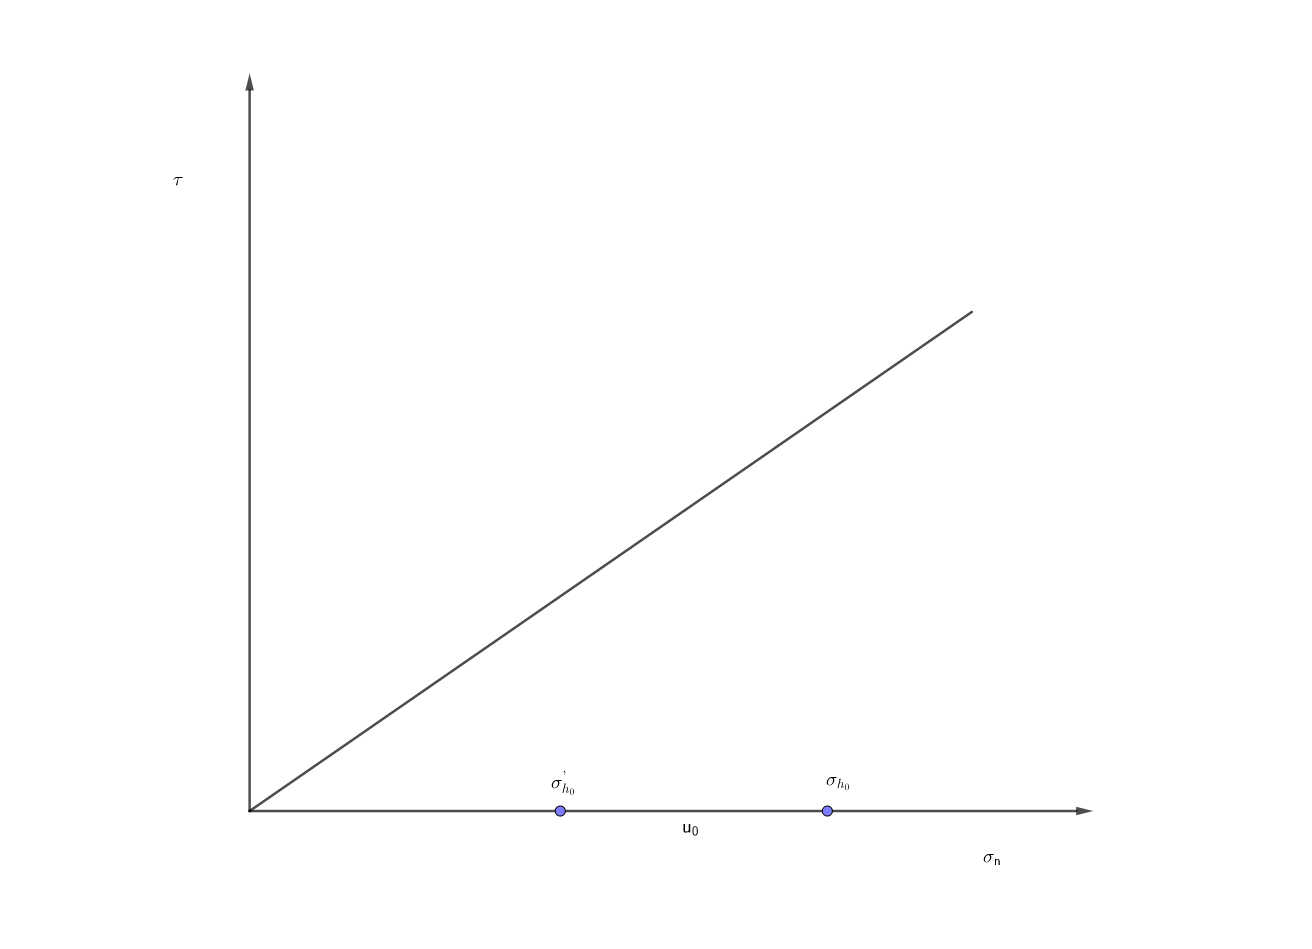
\includegraphics[width=\textwidth]{img/presio1}
		\caption{Estado inicial}
		\label{fig:presio1}
		\end{figure}
	\end{minipage}%
	\begin{minipage}{0.5\linewidth}
		\begin{figure}[H]
			\centering
			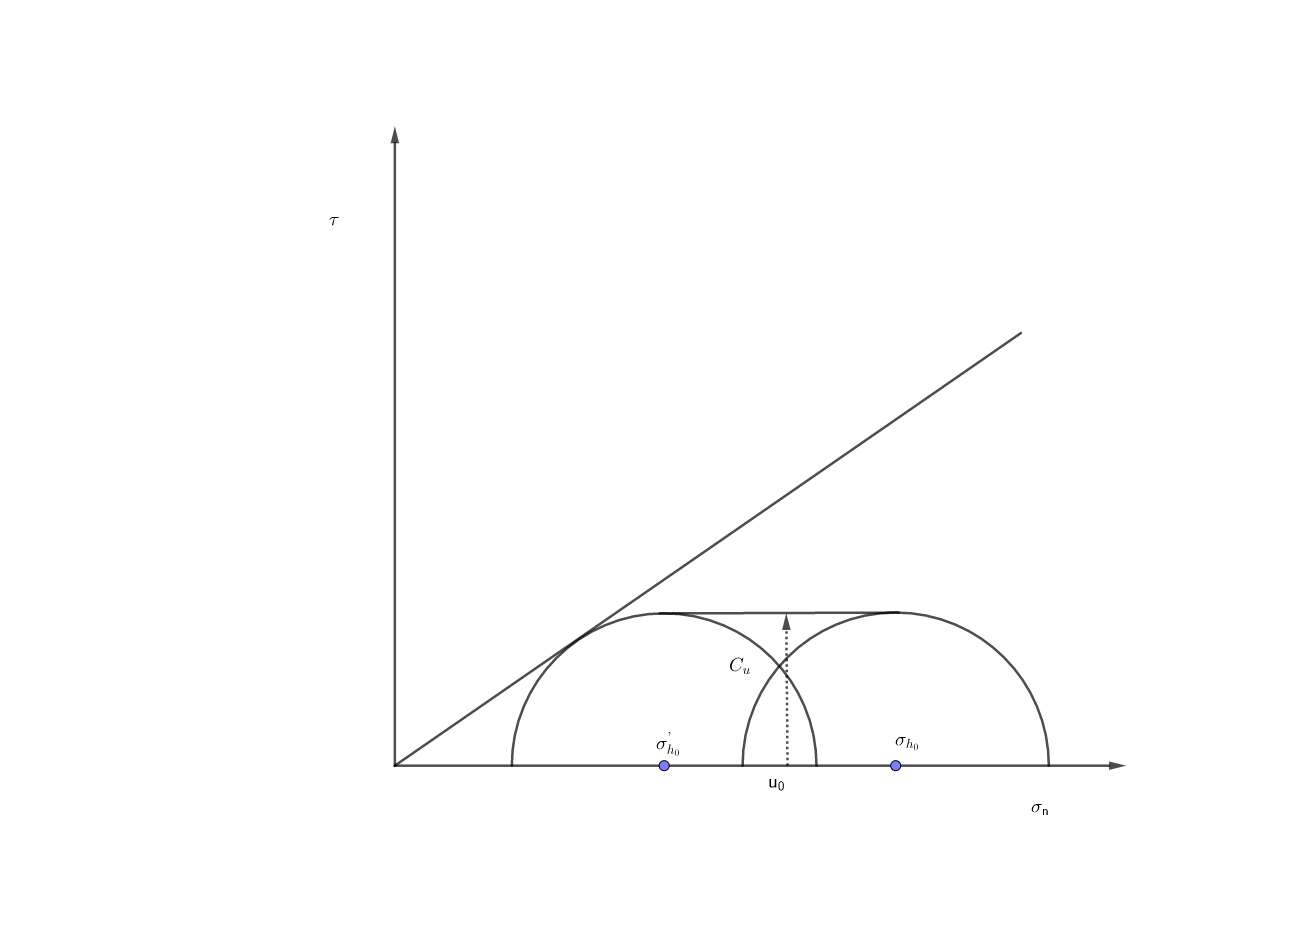
\includegraphics[width=\textwidth]{img/presio2}
			\caption{Incremento de presión con presión intersticial constante}
			\label{fig:presio2}
		\end{figure}
	\end{minipage}
	\begin{figure}[H]
			\centering
			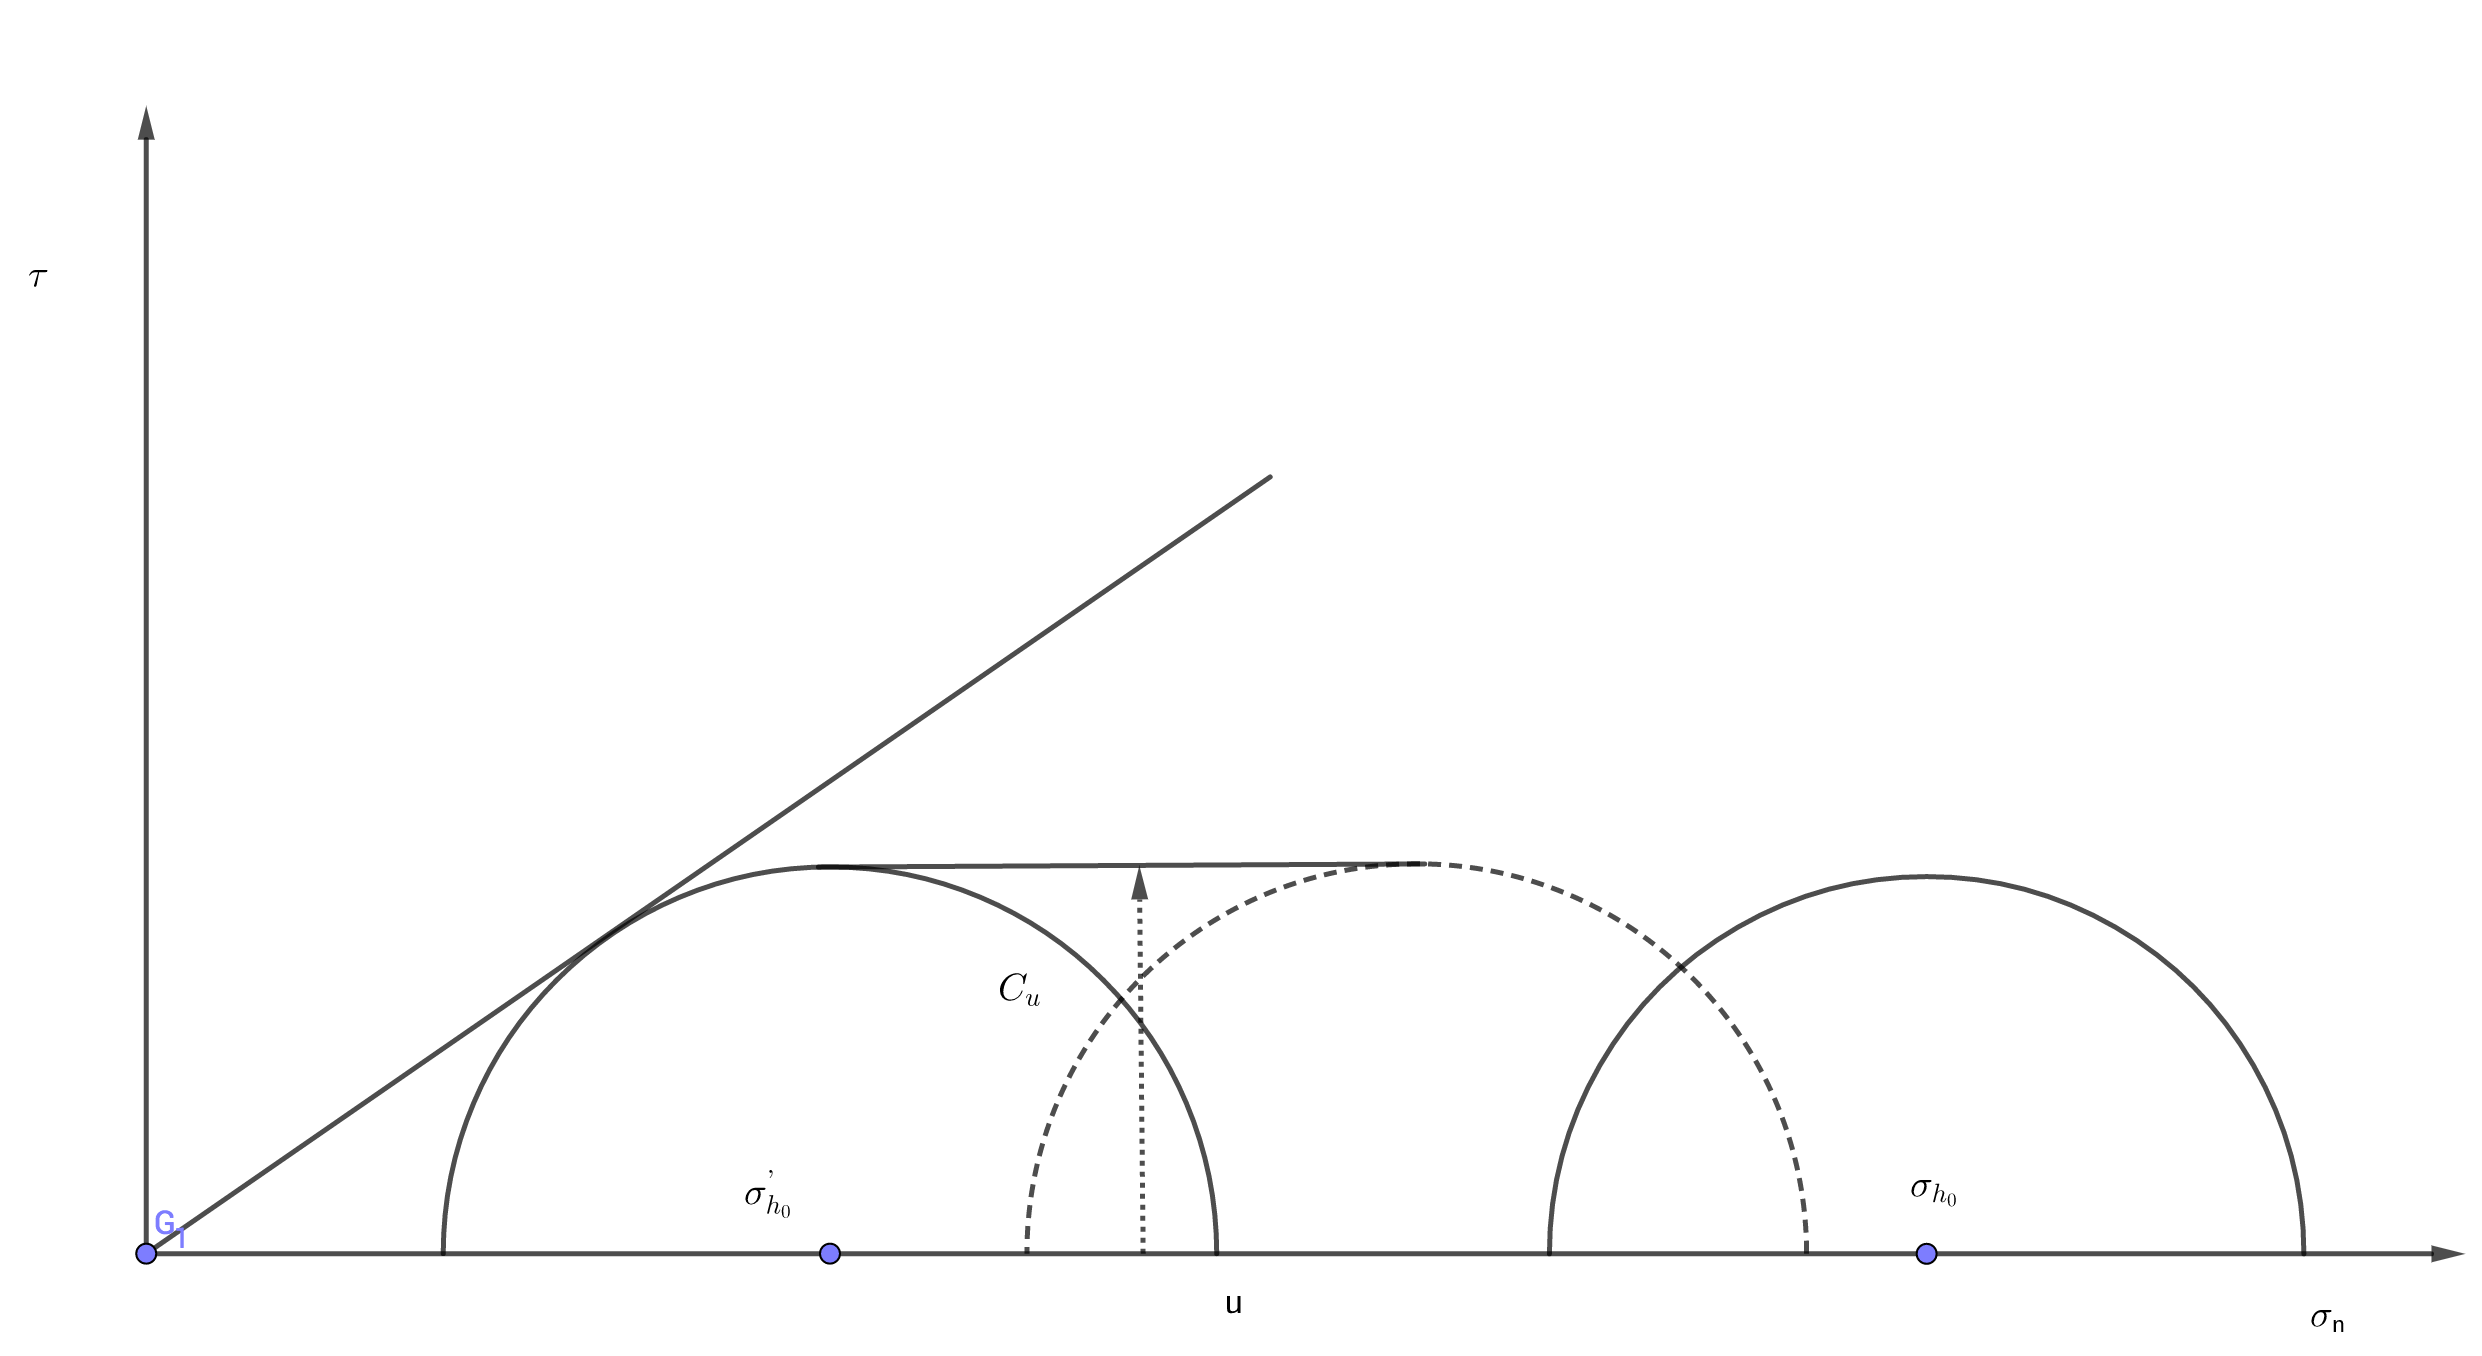
\includegraphics[width=0.6\textwidth]{img/presio3}
			\caption{Aumento de la presión intersticial}
			\label{fig:presio3}
	\end{figure}
}


% section questions (end)

\newpage

\section{Cimentaciones superficiales} % (fold)
\label{sec:parte_2}


\question{Indica las principales hipotésis del método edométrico para el cálculo de asientos de consolidación y describe brevemente su grado de validez.}{
	Hipótesis:
	\begin{enumerate}
		\item Cálculo de $\sigma_v$ por elasticidad.
		\item $\Delta u = \Delta \sigma_v = \Delta \sigma_v^{’}$, el aumento de presión interna es igual al aumente de presión vertical.
		\item Las tensiones totales se mantienen invariantes a lo largo de la consolidación.
	\end{enumerate}
	Es válido (muy usado) aunque la segunda hipótesis se distancia de la realidad.
	\begin{myrem}[Skempton-Bjerrum]
		Intenta mejorar el efecto de la segunda hipótesis.
	\end{myrem}
}


\question{Calcular FS de la cimentación cuadrada de la Figure~\ref{fig:cimen} en condiciones no drenadas utilizando carga neta. Comenta el resultado.}{
	Al estar en situación no drenada tenemos:
	\[
		q_r = C_u N_c + q
	\]
	\begin{figure}[H]
		\centering
		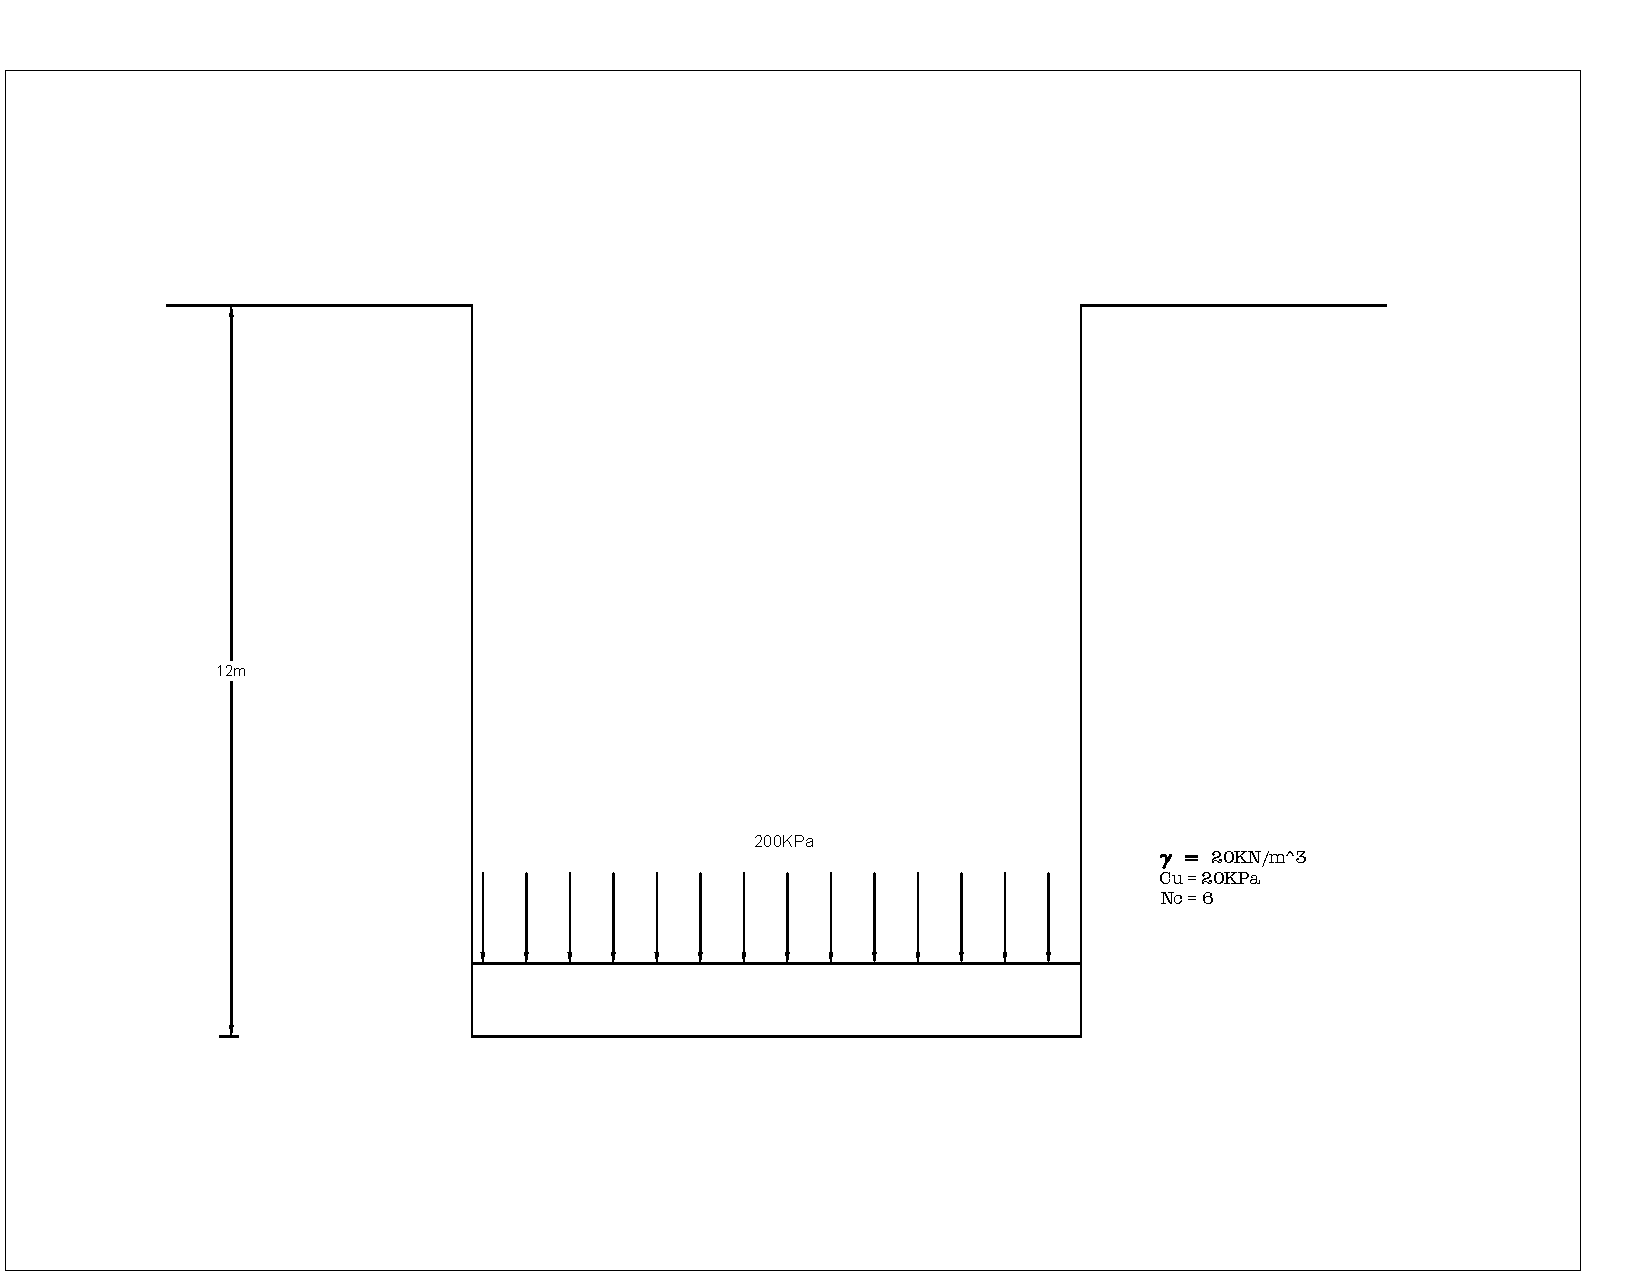
\includegraphics[width=0.9\textwidth]{img/capacidad_portante}
		\caption{Cimentación cuadrada}
		\label{fig:cimen}
	\end{figure}

	Tenemos (aplicando carga neta):
	\[
		FS = \frac{q_r - q}{q_{ad}-q} = \frac{360-240}{200 - 240} <0
	\]


	Lo cual es lógico ya que si analizamos la carga que este terreno soportaba antes de excavar observamos que era superior. Luego no hay razón de dudar de la estabilidad de esta cimentación.

	\begin{myrem}[FS real]
		Al calcular sin carga neta obtenemos
		\[
			FS = \frac{q_r }{q_{ad}} = \frac{360}{200} \approx 1,8
		\]
		Lo cual es incoherente con lo previamente comentado.
	\end{myrem}
}



\question{El asiento de una placa circular rígida sobre un semiespacio elástico homogéneo se expresa como $s=\frac{1-\mu^2}{2}\frac{P}{aE}$, donde s es el asiento, P la carga total aplicada, a el radio de la placa, E el módulo de elasticidad y $\mu$ el coeficiente de Poisson. Determinar la expresión para el módulo de balasto en estas condiciones. Comentar brevemente lo más destacado del resultado.}{
El módulo de balasto no es un parámetro del terreno. El módulo de balasto se puede determinar a partir de E,$\mu$ del terreno para una geometría dada. En este caso el el módulo de balasto variará en función del radio a.
	\[
		K = \frac{P}{s} = \frac{2aE}{1-\mu^2}
	\]
}

\question{La Figure~\ref{fig:ciment_larga} representa la cimentación cuadrada (6x6m) de una pila (circular de 2m de $\phi$) de un puente situado en un embalse. La cimentación alcanzaría su capacidad portante total si se aplicara una carga P de 1600T de forma rápida (condiciones no drenadas). ¿Con qué carga se alcanzaría la capacidad portante si el nivel del embalse estuviera 6m por encima del actual.}{
	\begin{figure}[H]
		\centering
		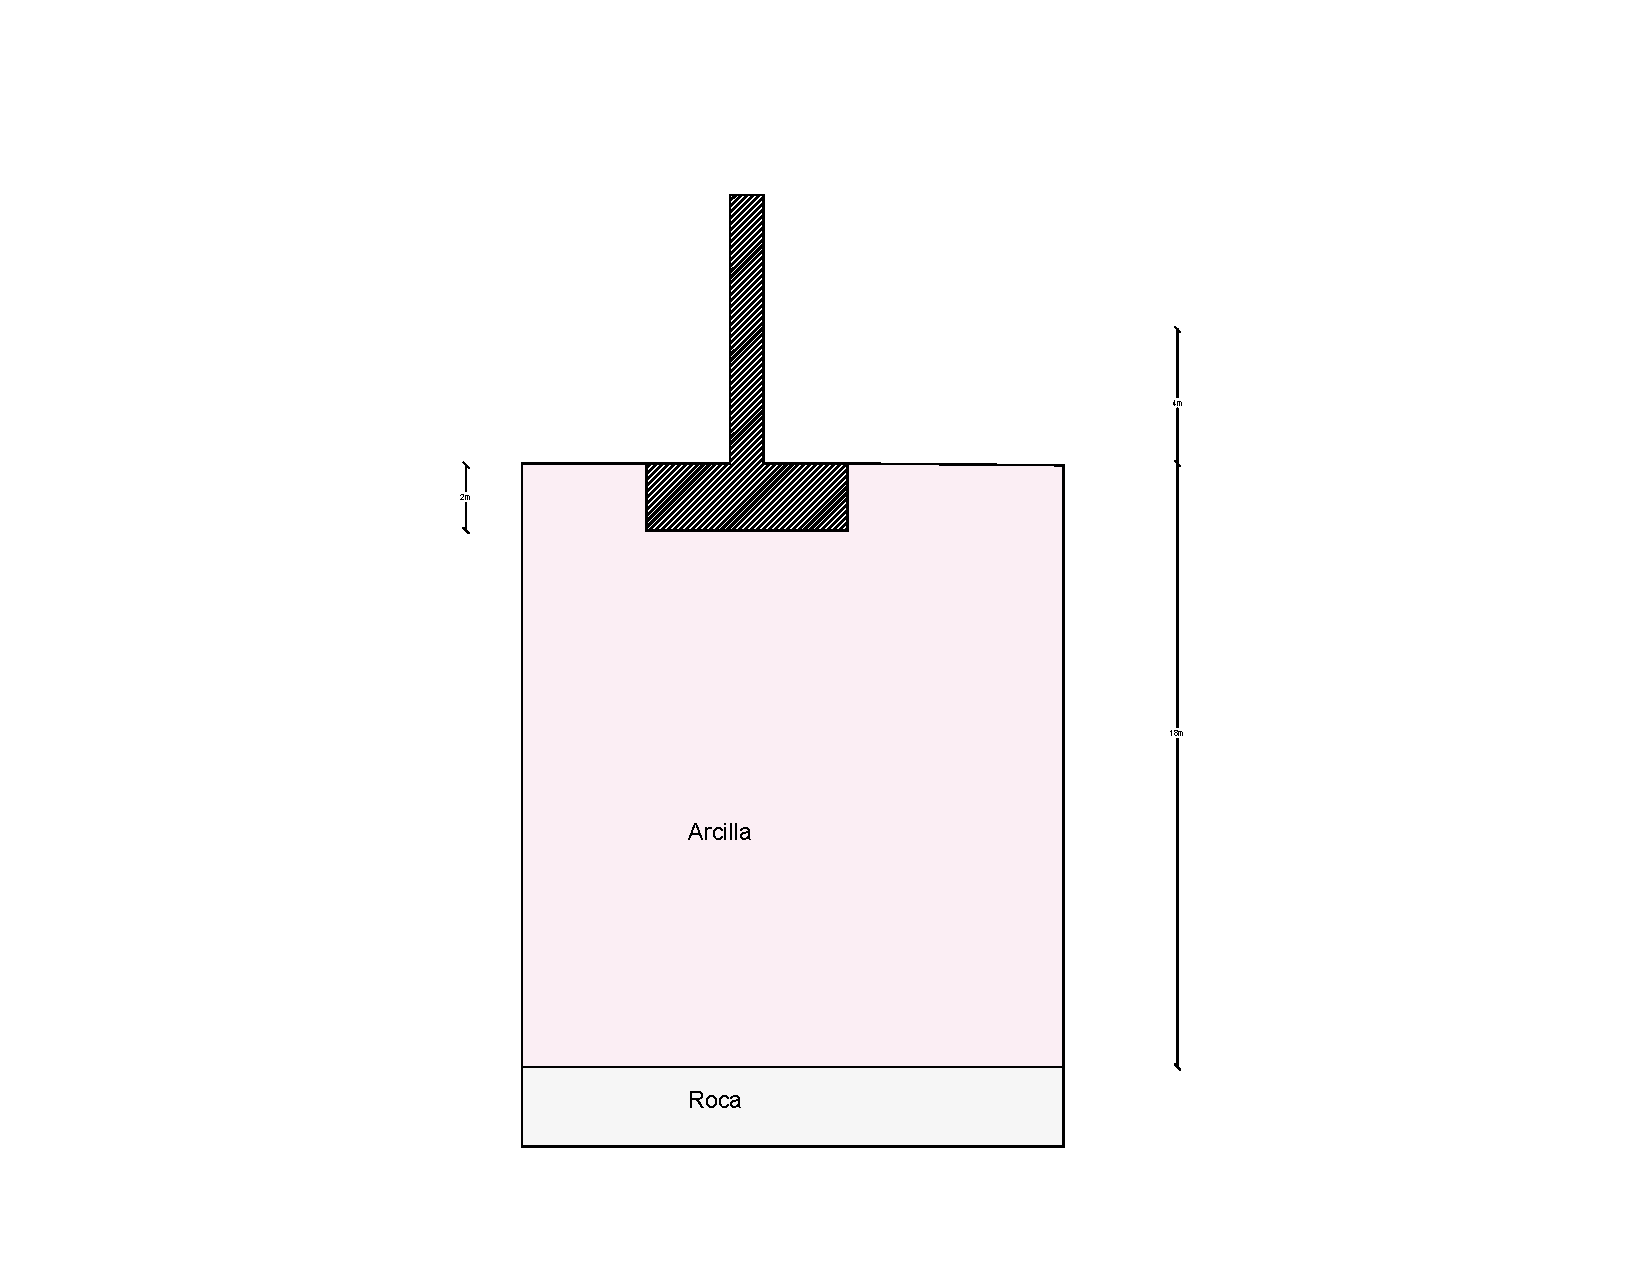
\includegraphics[width=0.5\textwidth]{img/cimentacion_larga}
		\caption{Cimentación cuadrada}
		\label{fig:ciment_larga}
	\end{figure}

	Al aplicarse rápidamente carga, nos situamos en condiciones drenadas. Analizaremos el problema en presiones totales y efectivas. Supondremos en ambos análisis $P = P_{peso-propio} + P_{peso aplicado}$

	\paragraph{Presiones totales} % (fold)
	\label{par:presiones_totales}
	
	\begin{multline}
		q_r = C_u N_c + \gamma_w H  = \frac{P + \gamma_w (H-h_b)(A_b - A_c)}{A_b}\\
		\Leftrightarrow P = C_u N_c A_b + \gamma_w (H- h_b) A_c + \gamma_w h_b A_b
	\end{multline}
	% paragraph presiones_totales (end)

	\paragraph{Presiones efectivas} % (fold)
	\label{par:presiones_efectivas}

	\begin{multline}
		q_r = C_u N_c  = \frac{P - \gamma_w h_b A_b - \gamma_w (H-h_b)(A_b - A_c)}{A_b}\\
		\Leftrightarrow P = C_u N_c A_b + \gamma_w (H- h_b) A_c + \gamma_w h_b A_b
	\end{multline}
	
	% paragraph presiones_efectivas (end)

	Luego tenemos 
	\[
		\Delta P = \gamma_w \Delta H A_c
	\]
}

\question{Si la carga se aplica lentamente (drenada), el valor de carga P con la que se alcanza la capacidad portante es de 12200T. ¿Con qué carga se alcanzaría la capacidad portante si el nivel del embalse estuviera 6m por encima de su nivel actual?}{
	A pesar de estar la capacidad portante en presiones efectivas, podemos trabajar en presiones totales o efectivas.
	\paragraph{Presiones totales} % (fold)
	\label{par:presiones_totales}
	\begin{multline}
		q_r^\prime + \gamma_w H = \frac{P  - \gamma_w (H-h_b)(A_b - A_c)}{A_b} \\
		\Leftrightarrow P = A_b q_r^\prime + \gamma_w H A_b  - \gamma_w (H-h_b)(A_b - A_c) \\
		\Leftrightarrow P = A_b q_r^\prime- \gamma_w H A_b h_b -  \gamma_w (H-h_b)A_c
	\end{multline}
	% paragraph presiones_efectivas (end)

	\paragraph{Presiones efectivas} % (fold)
	\label{par:presiones_efectivas}
	\begin{multline}
		q_r^\prime  = \frac{P -\gamma_w H A_b  - \gamma_w (H-h_b)A_c}{A_b} \\
		\Leftrightarrow P = A_b q_r^\prime- \gamma_w H A_b h_b -  \gamma_w (H-h_b)A_c
	\end{multline}
	% paragraph presiones_efectivas (end)

	Luego tenemos 
	\[
		\Delta P = -\gamma_w \Delta H A_c
	\]
}


\question{En el caso de la capacidad portante de una cimentación superficial ¿Qué caso es más crítico?
\begin{enumerate}
	\item Corto plazo 
	\item Largo plazo
\end{enumerate}}{
	El peor caso es a \emph{corto plazo} ya que como podemos ver en la Figure~\ref{fig:tensiones}, la trayectoria en tensiones totales (color verde) queda limitada por $C_u$. 
	\begin{figure}[H]
		\centering
		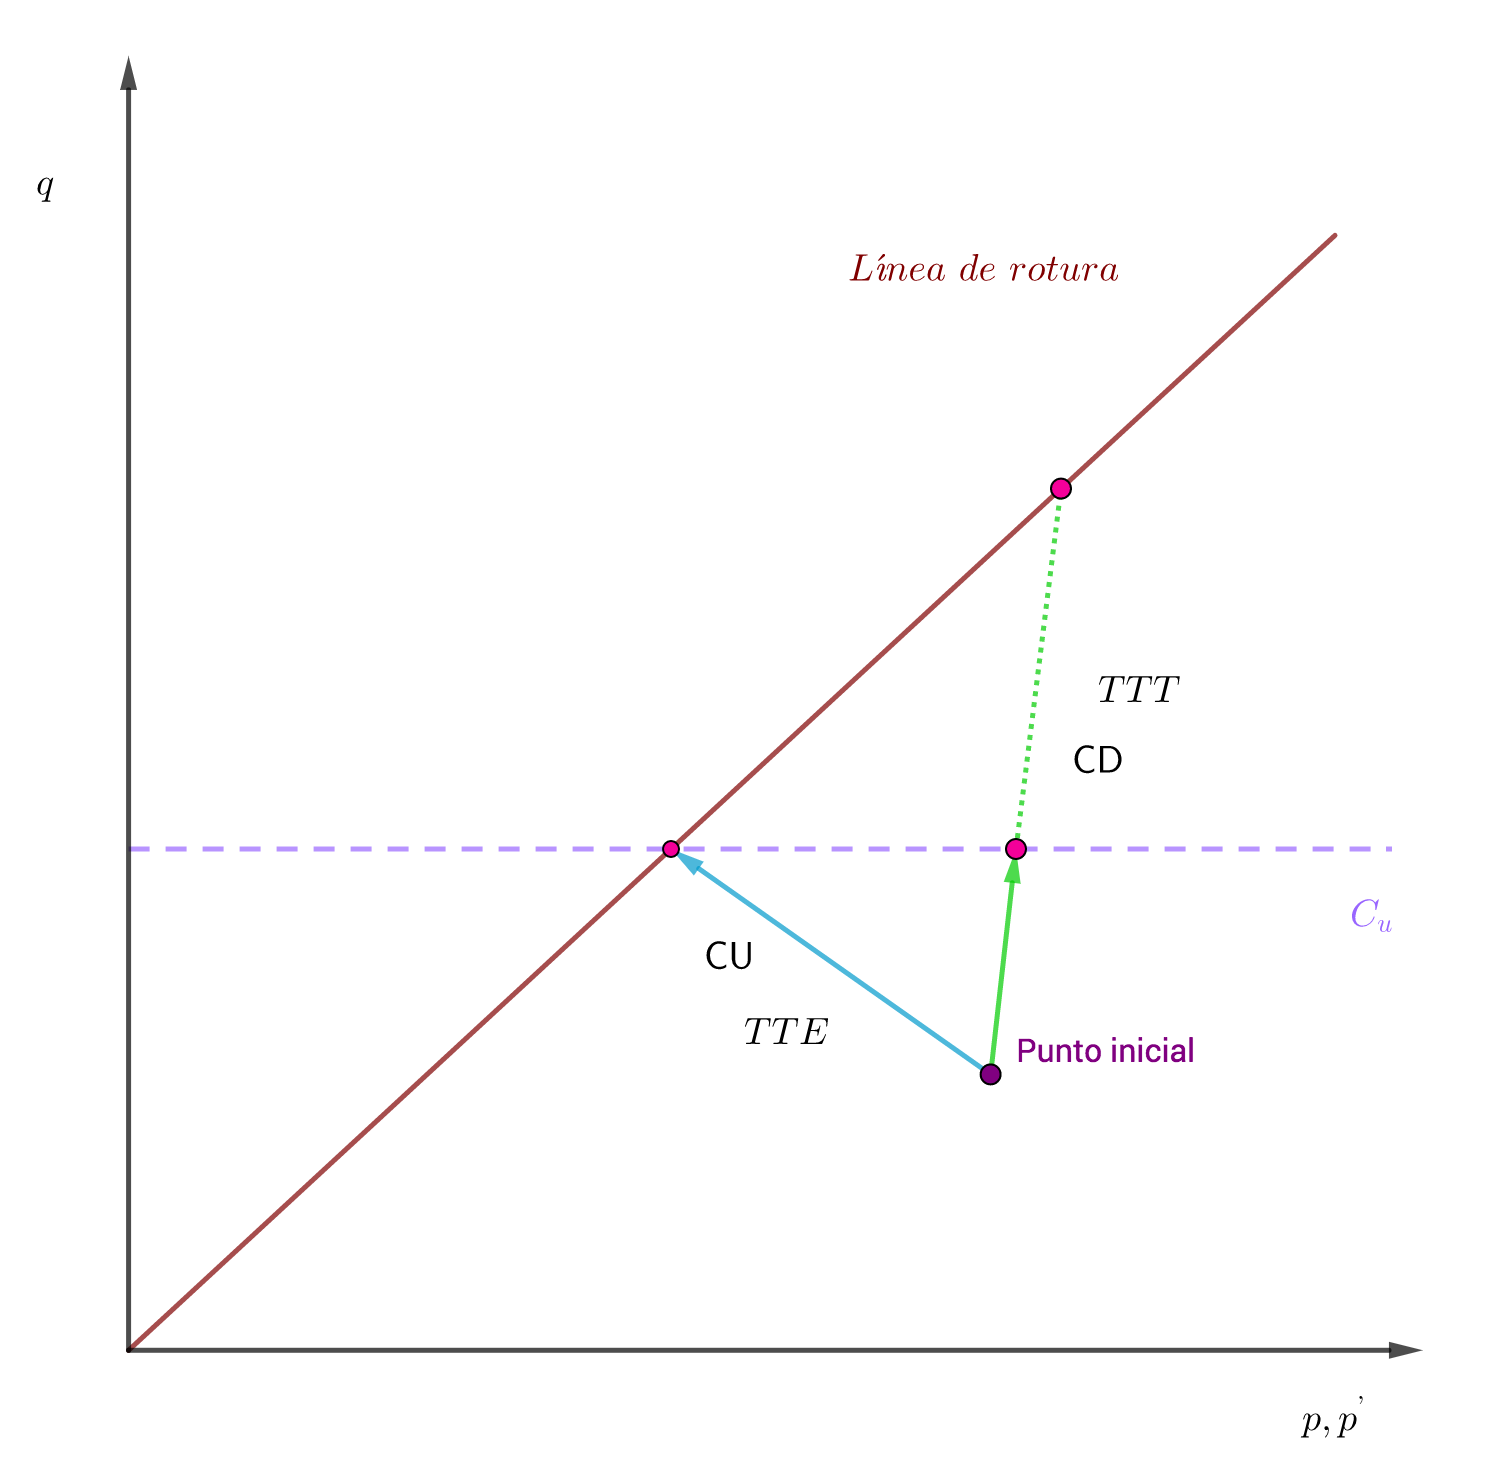
\includegraphics[width=0.5\textwidth]{img/trayectoria_tensiones}
		\caption{Trayectoria de tensiones }
		\label{fig:tensiones}
	\end{figure}
}

\question{Indica 3 posibles causas de deformación excesiva de una cimentación superficial no directamente relacionados con la carga aplicada}{
	\begin{enumerate}
		\item Levantamientos debidos a suelos expansivos o susceptibles a las heladas
		\item Deterioro del material de cimentación.
		\item Deformación por saturación de suelos colapsables (rellenos,loess)
		\item Deformación del terreno debido a excavaciones cercanas.
		\item Variación del NF
		\item Compactación del terreno por vibración, terremotos…
	\end{enumerate}
}

\question{La relación entre el asiento calculado por el método edométrico y por el método de Skempton es: 
\[
	S_{sb}= \mu S_{ed} = [A+\alpha (1-A)]S_{ed}
\]
Donde A es el parámetro de Skempton que depende de $\frac{z}{B}$. El valor de $\alpha$ para $\frac{z}{B}=0$ es 1. ¿Por qué?}{
	Una de las hipótesis del método edómetrico ($\epsilon_h = 0$) es que el incremento de presión intersticial es igual al incremento de presión vertical:
	\[
		\Delta u = \Delta \sigma_v
	\]
	El método de Skempton trata de mejorar esta aproximación introductiendo el parámetro $\mu = [A+\alpha (1-A)]$. Donde:
	\[
		\alpha \in[0,1] \propto 1-\frac{z}{B}
	\]
	En efecto si $\frac{z}{B}=0$, es decir la base es mucho mayor que la dimensión vertical del estrato (potencia), entonces nos situamos en condiciones edometricas y los asientos deben coincidir $\Rightarrow \alpha = 1$.
}


\question{Una placa de $\phi = 0,2m$ sometida a $10 T/m^2$ sufre un asiento de $0,2cm$. ¿Qué asiento se obtendrá al cargar una cimentación de $\phi = 1,2m$ y $20T/m^2$. Suponiendo suelo elástico-lineal?}{
	Tenemos $s \propto Q$ así pues:
	\[
		s_2 = s(2Q) = 2s(Q) = 2s_1
	\]
	Al tener un suelo elástico lineal $\frac{B}{s}=cte$, luego:
	\[
		s_3 = \frac{B_3}{B_2}s_2 
	\]	
	Luego mediante aplicación numerica $s_3 \approx 2,4cm$
}


\question{ En la práctica. ¿Esperarías que el asiento de la cimentación fuera mayor o menor que el calculado? ¿Por qué?}{
	La teoría elástico lineal no tiene en cuenta la variación del módulo elástico con la profundidad ($\frac{dE}{dz}>0$), luego es de esperar un asiento menor en la práctica.
}

\question{Las expresiones de la capacidad portante tienen la siguiente estructura (en terreno drenado):
\[
	q_r = cN_c + \frac{1}{2}\gamma B N_\gamma + qN_q
\]
}{
	\begin{enumerate}
	\item ¿A qué mecanismo de resistencia corresponde cada uno de los términos?
		\begin{enumerate}
			\item Contribución de la cohesión del suelo a la resistencia
			\item Efecto del peso
			\item Contribución de cargas sobre el plano de cimentación
		\end{enumerate}
	\item ¿Qué forma adopta en el caso de un terreno sumergido?
		En el caso de un terreno submergido hemos de tener en cuenta el efecto del empuje de Arquimedes, así pues podemos trabajar en tensiones efectivas:
		\begin{equation}
			\begin{cases}
				q_r^{’}=c^{’}N_c + \frac{1}{2}\gamma^{’} B N_\gamma + q^{’}N_q\\
				q_r =q_r^{’} + (p_w)_{base} 
			\end{cases}
		\end{equation}
	\item ¿Qué forma adopta en el caso de un análisis no drenado en tensiones totales $\phi = 0$
	Tenemos $N_q(\phi = 0)=1, N_\gamma(\phi = 0)=0$, luego:
	\[
		q_u = C_u N_c + q
	\]
	\item ¿Qué forma adoptaría q en el caso que el terreno de cimentación fuera exclusive agua?
	\begin{equation}
		\begin{cases}
			q_r =q_r^{’} + (p_w)_{base} = c^{’}N_c + \frac{1}{2}\gamma^{’} B N_\gamma + \gamma_w H_w, &\text{ drenado}\\
			q_r = C_uN_c + \gamma_w H_w,&\text{ no drenado}
		\end{cases}
	\end{equation}
\end{enumerate}
}

% section parte_2 (end)

\newpage

\section{Cimentaciones profundas} % (fold)
\label{sec:cimentaciones_profundas}

\begin{mybox}{Pilotes}
Es la máxima presión que puede sufrir el terreno bajo la cimentación
\tcbsubtitle{\emph{CPI 4}}
	\begin{enumerate}
		\item Avance tubería con cuchare o trépano
		\item Empotramiento del pilote
		\item Hormigonado y extracción de la tubería
	\end{enumerate}
\tcbsubtitle{\emph{CPI 7}}
	\begin{enumerate}
		\item Avance de la perforación con el auger
		\item Hormigonado
	\end{enumerate}
	\begin{myrem}[Restricción]
		El terreno ha de tener cierta cohesión
	\end{myrem}
\tcbsubtitle{\emph{CPI 8 (barrena continua)}}
	\begin{enumerate}
		\item Introducimos la barrena a rotación hasta el fondo (donde se quiere llegar)
		\item Se hormigona mientras se va quitando la barrena
		\item Introducción de la armadura en el hormigón fresco
	\end{enumerate}
	\begin{myrem}[Armaduras]
		Suelen trabajar a compresión, luego si la armadura no es más corta no tiene porque ser problemático.
	\end{myrem}
\tcbsubtitle{\emph{CPI 3 (hincado)}}
	\begin{enumerate}
		\item Hincado
		\item Formación del bulbo
		\item Hormigonado y extracción de la tuberia
	\end{enumerate}
\end{mybox}

\begin{figure}[H]
		\centering
		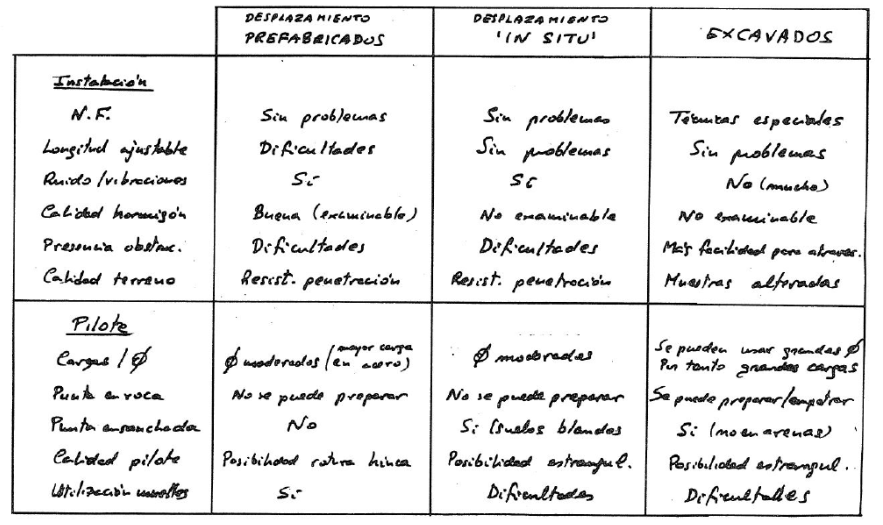
\includegraphics[width=\textwidth]{img/compar}
		\caption{Comparación de los distintos métodos}
		\label{fig:compar}
\end{figure}

\begin{mybox}{Método Delft}
	\begin{ldef}[Delft]
		Permite calcular la resistencia en punta de un pilote
	\end{ldef}

	La resistencia no es uniforme, así pues solemos estimar un único valor medio de la distribución.

	\tcbsubtitle{\emph{Procedimiento}}

	Se definen 3 zonas, de menor a mayor profundidad y se cálcula
	\begin{equation}
		\begin{cases}
			q_c = \frac{(q_c)_{I}+(q_c)_{II}}{2}, &\text{ if }(q_c)_{III} >(q_c)_{II} \\
			q_c = \frac{(q_c)_{I}+\frac{(q_c)_{II}+(q_c)_{III}}{2}}{2}, &\text{ if }(q_c)_{III} \leq(q_c)_{II}
		\end{cases}
	\end{equation}
\end{mybox}

% section cimentaciones_profundas (end)

\newpage



\section{Coeficiente de empuje} % (fold)
\label{sec:parte1}

\question{Explicar en pocas palabras 3 posibles métodos pasa calcular el empuje adicional causado por sobrecargas externas}{
	\begin{itemize}[label=\ding{69}]
		\item Uniforme:
		\begin{figure}[H]
			\centering
			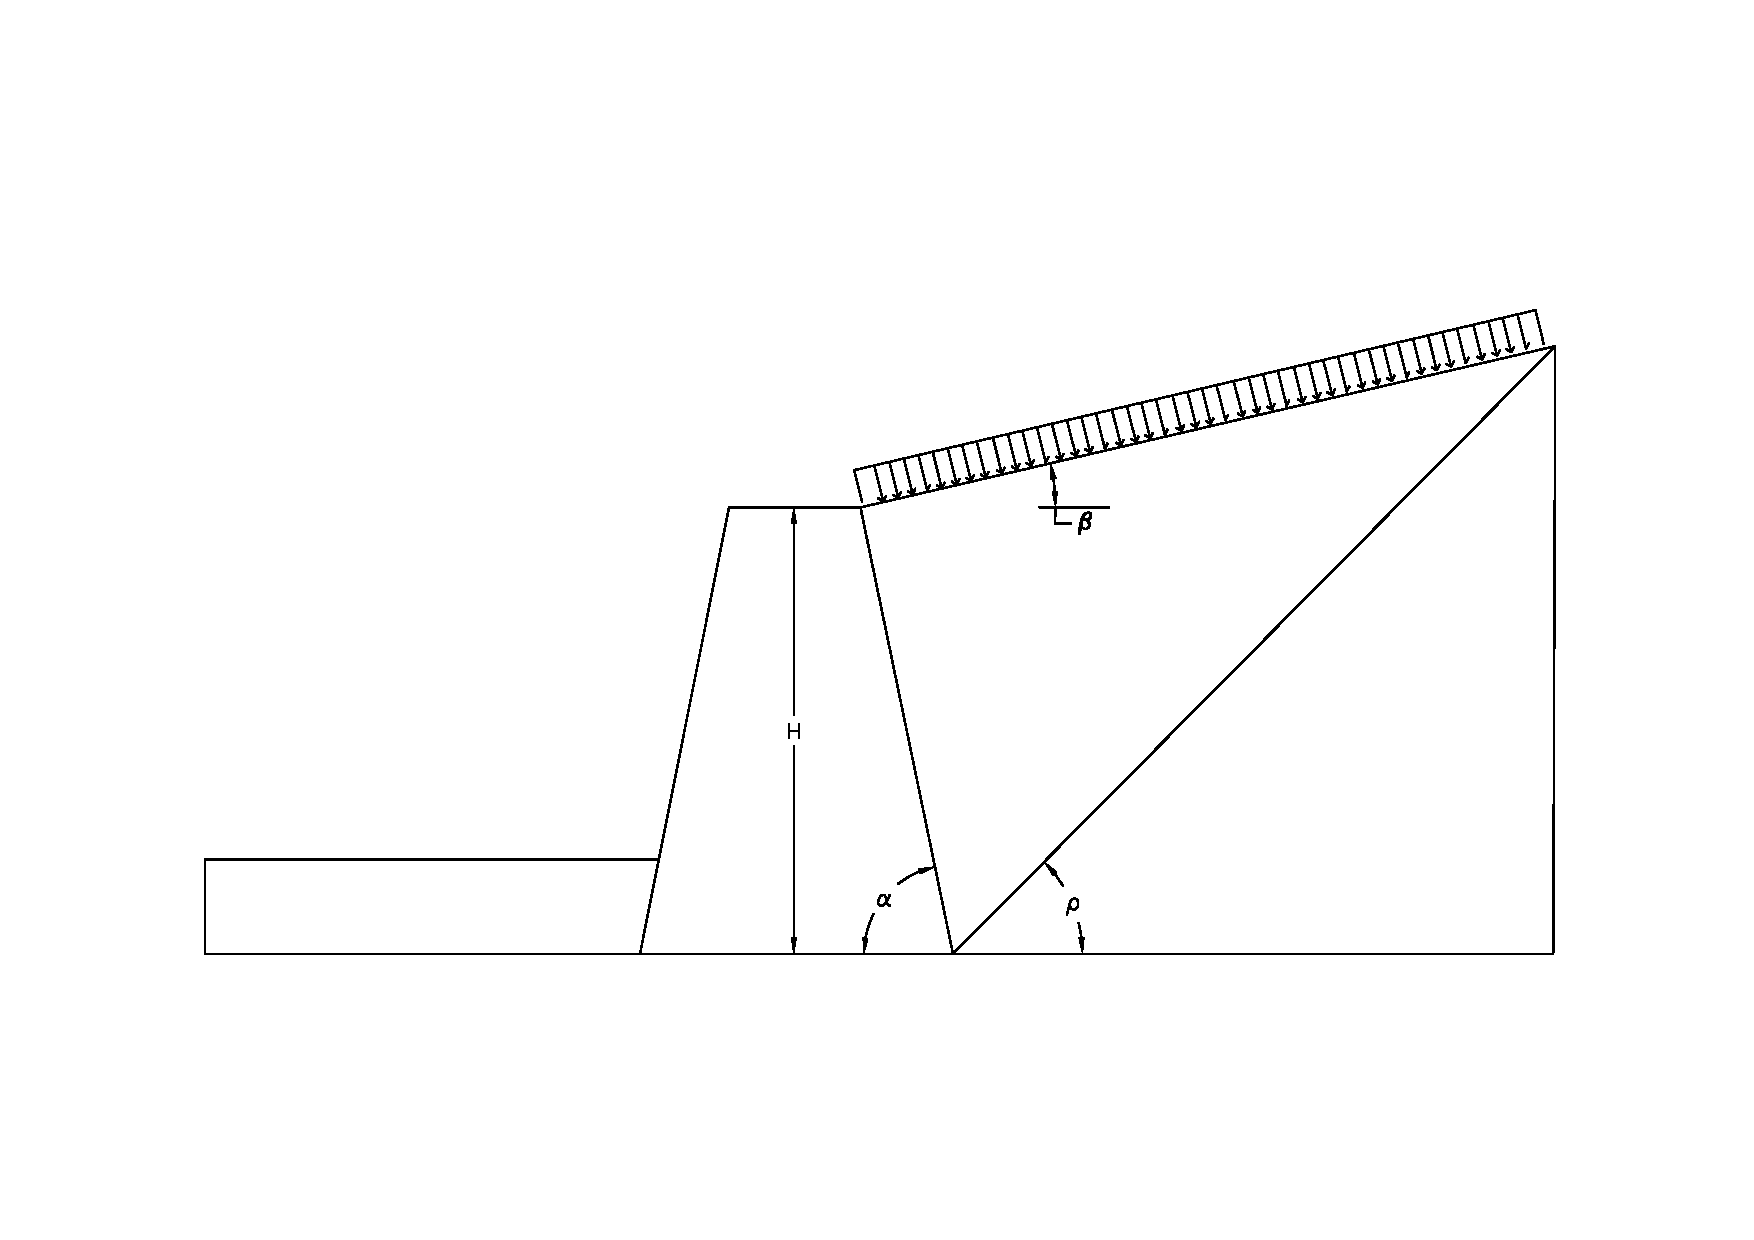
\includegraphics[width=0.7\textwidth]{img/cargas_uni}
			\caption{caption}
			\label{fig:Cargas uniformes}
		\end{figure}
		\[
			\gamma^{eq} = \gamma \frac{2q \sin(\alpha)}{H \sin(\alpha + \beta)}, \quad \emph{una densidad equivalente}
		\]
		O bien
		\[
			\Delta H = \frac{q \sin(\alpha)}{H \sin(\alpha+\beta)}, \quad \emph{una altura equivalente}
		\]
		\item No uniforme:
		\begin{figure}[H]
			\centering
			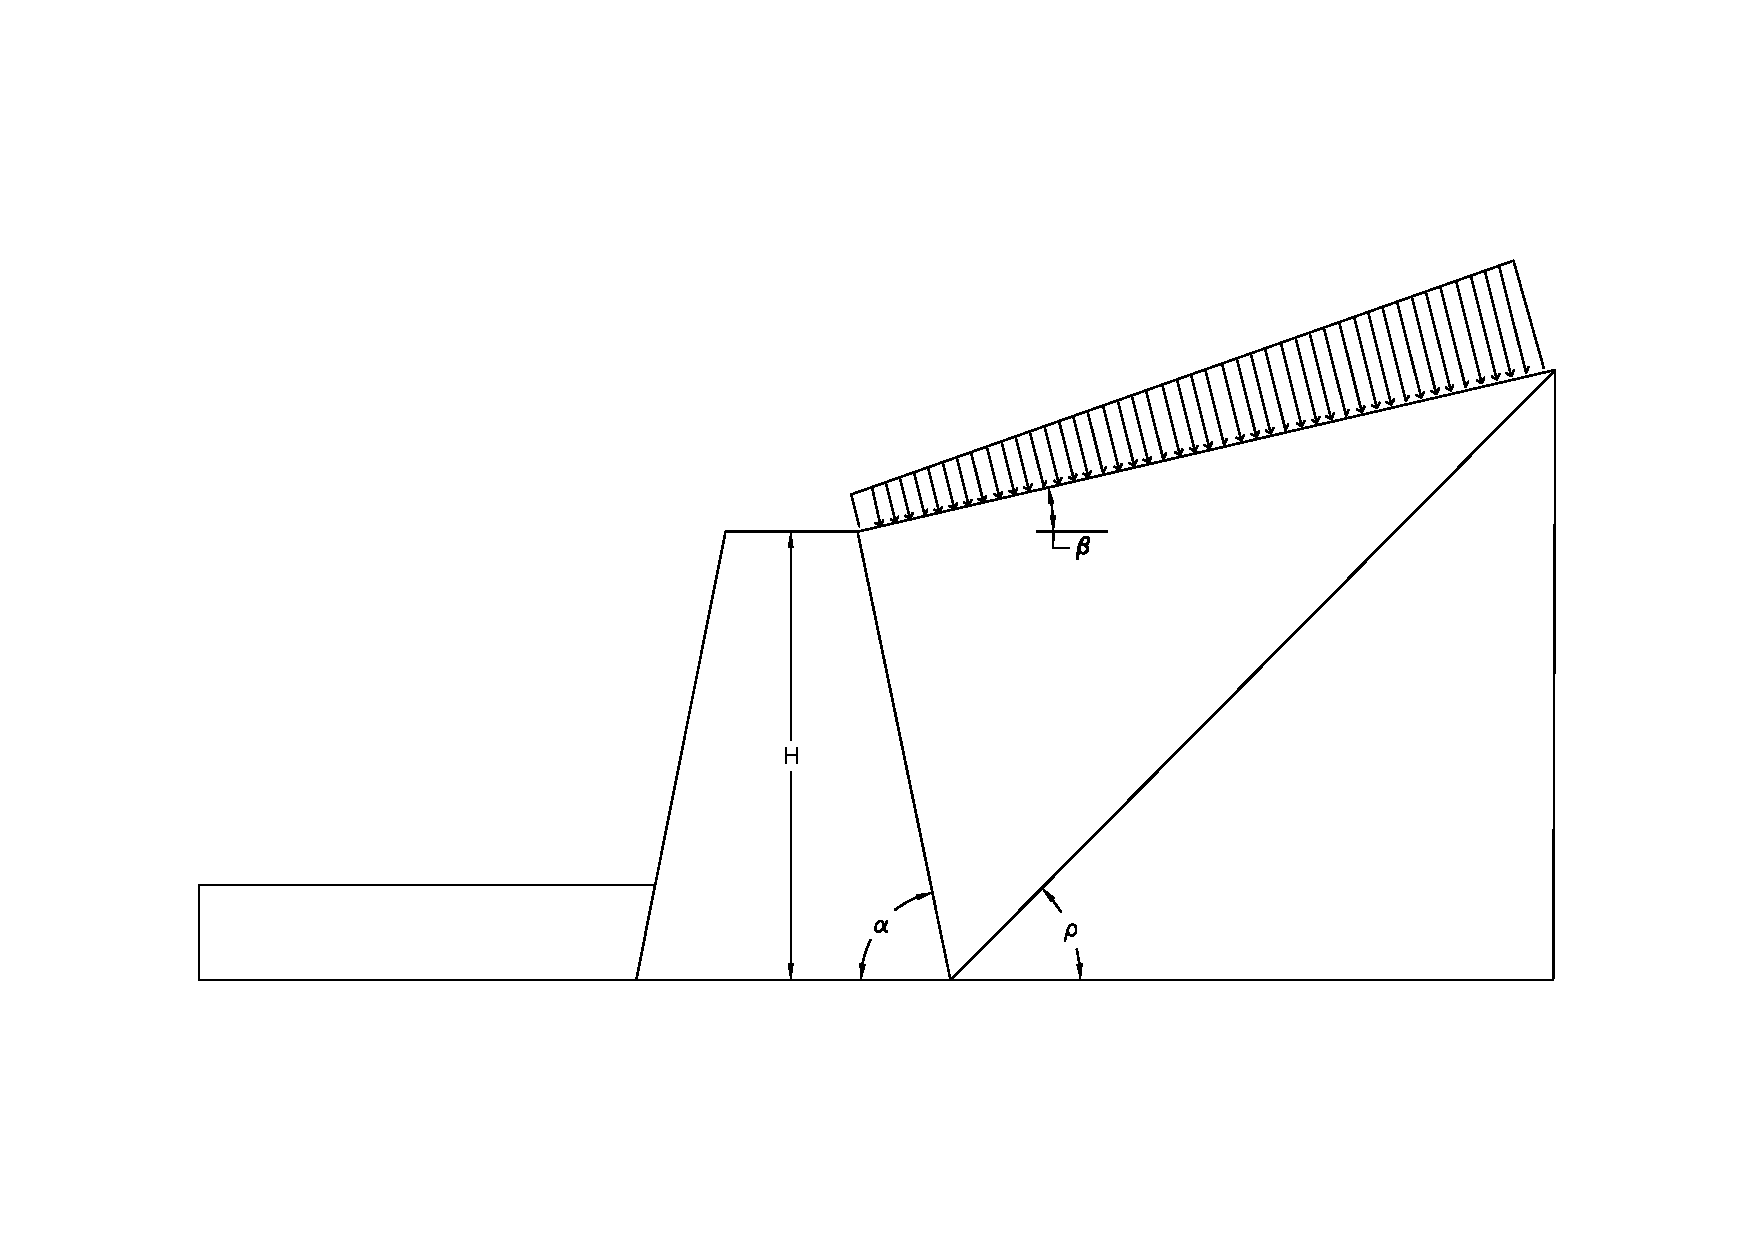
\includegraphics[width=0.7\textwidth]{img/cargas_no_uni}
			\caption{Cargas no uniformes}
			\label{fig:label}
		\end{figure}
		\begin{itemize}[label=\ding{71}]
			\item Soluciones elásticas (Boussinesq)
			\item Soluciones plásticas
			\item Reglas empíricas
		\end{itemize}
	\end{itemize}
}

\question{ Un muro con alto ángulo de rozamiento (40) está en contacto con un suelo de ángulo de fricción igual a 30. a) ¿ Qué valor escogerías como ángulo de rozamiento suelo-muro ? }{
	a)
	\[
		\delta = \frac{2}{3} \phi^{’}= 20
	\]
	b)
}

\question{¿ Qué diferencia conceptual existe entre el método de Coulomb y el de Rankine para el cálculo de empuje de tierras ? }{
	\begin{itemize}[label=\ding{69}]
		\item Rankine: 
		\begin{enumerate}
			\item no se considera rozamiento suelo-muro ($\delta=0$)
			\item se supone rotura completa del suelo
		\end{enumerate}
		\item Coulomb:
		\begin{enumerate}
			\item consideramos rozamiento suelo-muro ($\delta \neq 0$)
			\item Rotura según 2 planos, uno de ángulo $\rho$ y otro con el muro
		\end{enumerate}
	\end{itemize}
}

\question{Enumerar las razones por las que el metodo de Rankine es más seguro que el de Coulomb para el cálculo de empujes de tierras.}{
	\begin{enumerate}
		\item En el caso \textbf{pasivo} no es aconsejable usar Coulomb, pues sobre-estima lo que va a resistir el terreno 
		\[
			K_{pc}>K_{p-real} \Rightarrow E_{pc}>E{p-real}
		\]
		\item Rankine supone $\delta = 0 \Rightarrow$ \textbf{empuje activo máximo} ($\nexists$ componente estabilizadora del empuje) en la teoría de Coulomb supone parte del empuje como estabilizador 
		\[
		 	E_{Rankine} > E_{Coulomb}
		 \] 
		 \item Rankine supone rotura en todo el terreno, mientra Coulomb solo la considera en 2 lineas.
	\end{enumerate}
	Así pues el terreno rompe antes de lo que dica Coulomb.
}

\question{Cúal es la influencia de la fricción suelo-muro sobre: 
\begin{itemize}[label=\ding{69}]
	\item Empuje activo
	\item Empuje pasivo
	\item $K_0$
	\item Momento de vuelco por empuje activo
\end{itemize}}{
	\begin{itemize}[label=\ding{69}]
		\item \emph{Empuje activo:}
		\[
			\delta \approx \frac{2}{3} \phi^{’}
		\] 
		y 
		\[
			K_a = \frac{1- \sin(\phi^{’})}{1+ \sin(\phi^{’})} \Rightarrow \frac{\dif K_a}{\dif\phi^{’}}<0
		\]
		Con lo cual 
		\[
			\frac{\dif E_a}{\dif\delta}<0
		\]
		\item \emph{Empuje pasivo:}
		\[
			K_p = \frac{1+ \sin(\phi^{’})}{1+ \sin(\phi^{’})} \Rightarrow \frac{\dif K_a}{\dif\phi^{’}}>0
		\]
		Con lo cual 
		\[
			\frac{\dif E_p}{\dif\delta}>0
		\]
		\item $K_0$:
		No influye al estar en reposo
		\item \emph{Momento de vuelco por empuje activo}:
		\[
			\frac{\dif E_a}{\dif\delta}<0 \Rightarrow \frac{\dif M}{\dif\delta}<0
		\]
	\end{itemize}
}

\question{Dibujar cualitativamente la ley de empujes de Rankine sobre el muro de la Figure~\ref{fig:emp_gravedad}}{
	\begin{figure}[H]
		\centering
		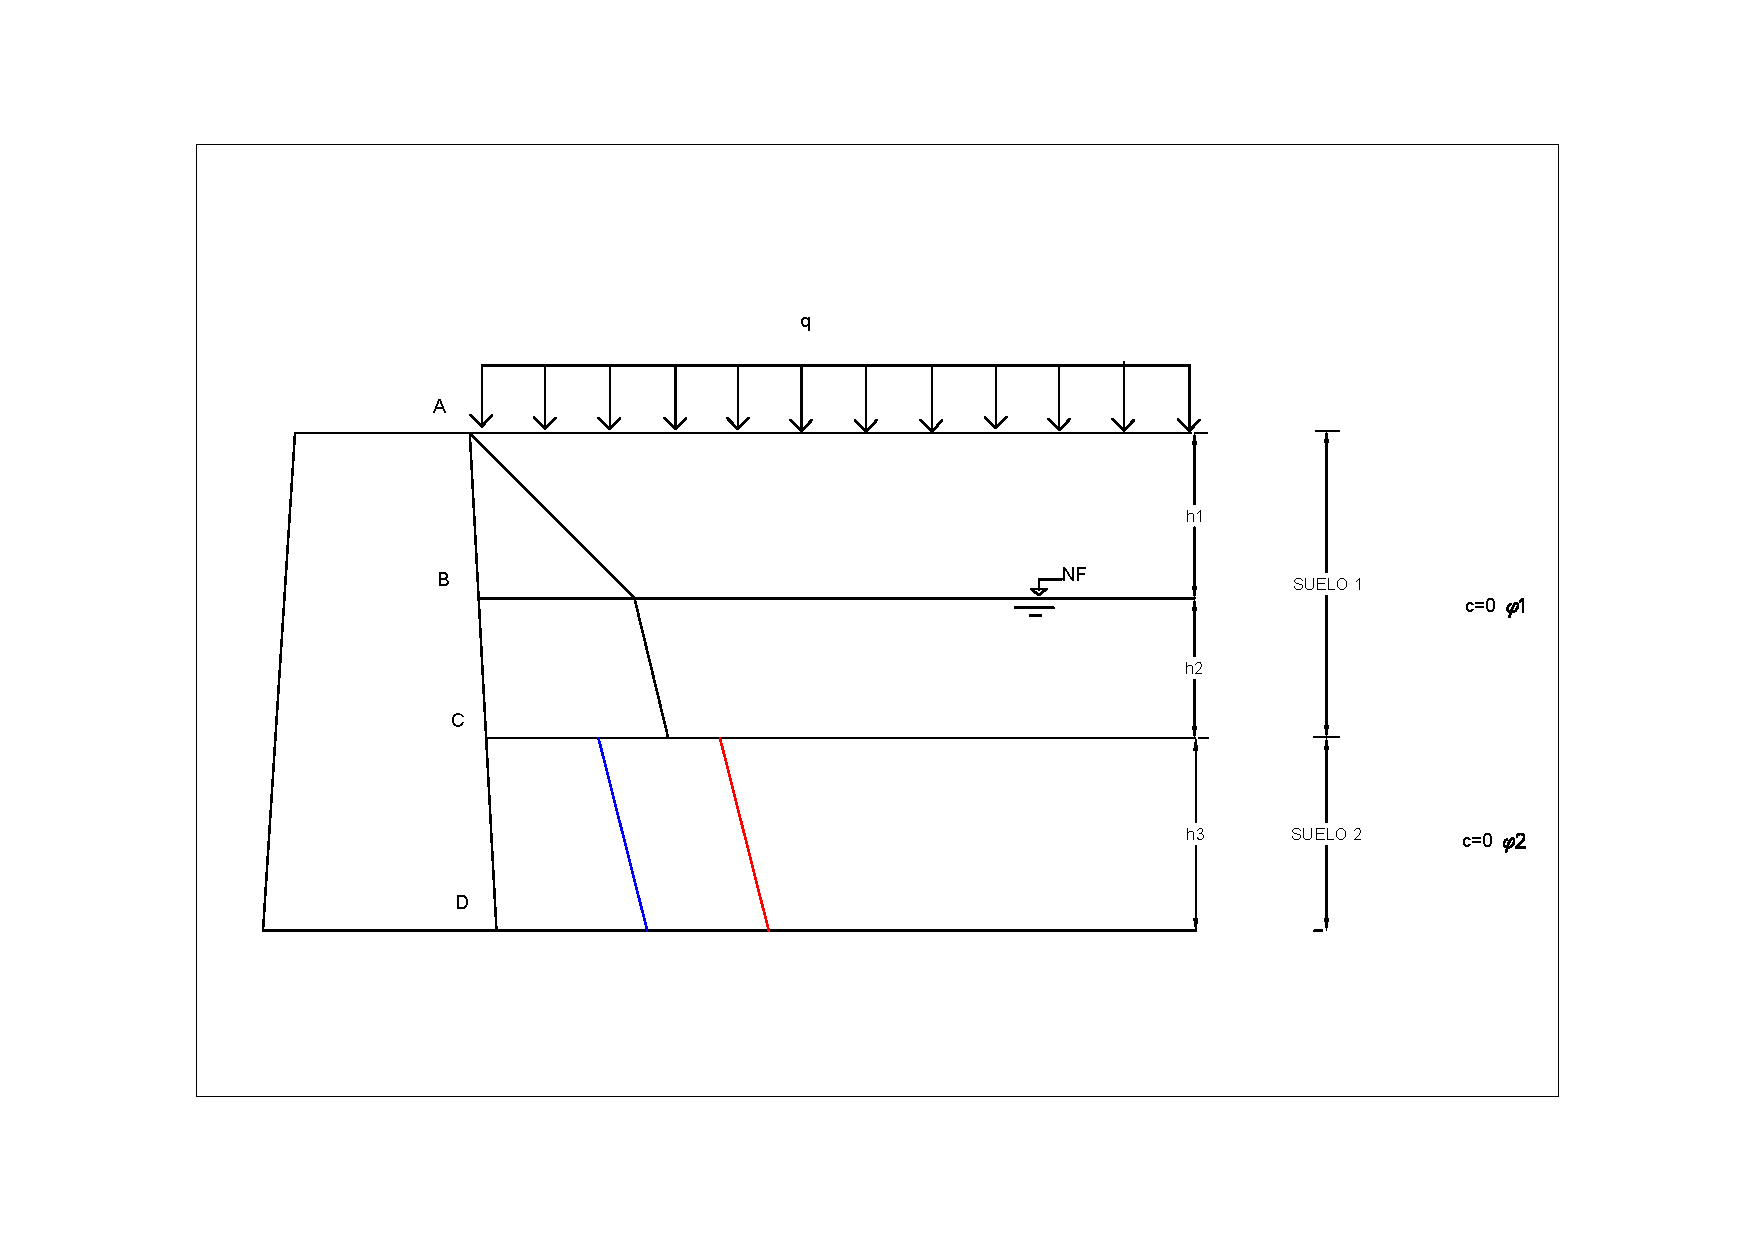
\includegraphics[width=0.9\textwidth]{img/ejemplo_empuje}
		\caption{Empuje de tierras sobre muro de gravedad}
		\label{fig:emp_gravedad}
	\end{figure}
	Tenemos:
	\begin{itemize}
		\item A: 
		\[
			\sigma_v^{’} = 0 \Rightarrow \sigma_h^{’}=0
		\]
		\item B:
		\[
			\sigma_v^{’} = \gamma h_1 + q \Rightarrow \sigma_h^{’}= K_a(\gamma h_1 + q)
		\]
		\item C:\\
		\emph{Parte superior:}
		\[
			\sigma_v^{’} = \gamma h_1 + \gamma^{’}h_2 + q \Rightarrow \sigma_h^{’}= K_a^{\phi_1}(\gamma h_1 + \gamma^{’}h_2+ + q)
		\]
		\emph{Parte inferior:}
		\[
			\sigma_v^{’} = \gamma h_1 + \gamma^{’}h_2 + q \Rightarrow \sigma_h^{’}= K_a^{\phi_2}(\gamma h_1 + \gamma^{’}h_2+ + q)
		\]
		\item D:
		\[
			\sigma_v^{’} = \gamma h_1 + \gamma^{’}(h_2+ h_3) + q \Rightarrow \sigma_h^{’}= K_a^{\phi_2}(\gamma h_1 + \gamma^{’}(h_2+ h_3) + q)
		\]

		\begin{myrem}
			En rojo el caso en el que $\phi_2 < \phi_1$ y en azul el contrario. En efecto tenemos $\frac{\dif K_a}{\dif\phi^{’}}>0$. Luego la variación de pendiente se debe a $\gamma^{’} < \gamma$
		\end{myrem}
	\end{itemize}
}

\question{Indicar qué parametros o propiedades fundamentales del terreno controlan el valor de $K_0$. ¿ Cómo varía $K_0$ con ellos ?}{

	EL grado de consolidación, $\phi^{’}$ y $I_p$. En el caso de tener una arcilla NC podemos considerar $K_0 = 1 - \sin(\phi^{’})$.

	\begin{minipage}{0.5\linewidth}
		\begin{figure}[H]
		\centering
		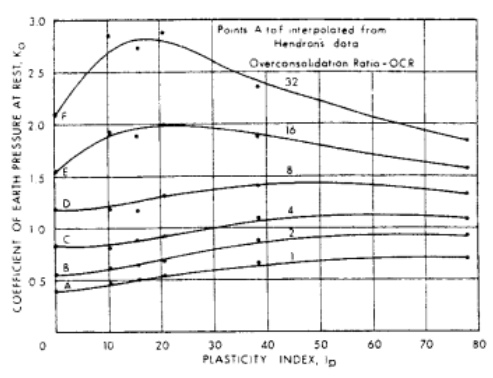
\includegraphics[width=\textwidth]{img/im1}
		\caption{caption}
		\label{fig:label}
		\end{figure}
	\end{minipage}%
	\begin{minipage}{0.5\linewidth}
		\begin{figure}[H]
			\centering
			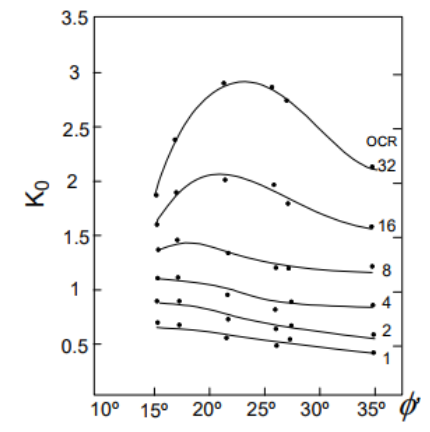
\includegraphics[width=\textwidth]{img/im3}
			\caption{caption}
			\label{fig:label}
		\end{figure}
	\end{minipage}
	
	\begin{figure}[H]
		\centering
		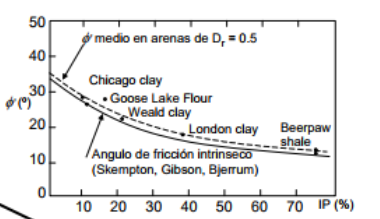
\includegraphics[width=0.5\textwidth]{img/im2}
		\caption{caption}
		\label{fig:label}
	\end{figure}
}

\question{¿ Cómo determinarías $K_0$ en laboratorio ? }{
	\begin{itemize}
		\item Ensayos edometricos
		\item Evaluación mediante succión (atención a la disminución de humedad)
	\end{itemize}
}

\question{ ¿ Podrías mencionar algún error conceptual que se admite en el desarollo del método del círculo de fricción para el cálculo del empuje pasivo ? Razonar para el caso c=0}{
	En el caso de empule pasivo en arcillas a largo plazo (c=0). Calcularemos el empuje pasivo como la suma de 2 estados:
	\begin{enumerate}
		\item Sólo interviene el peso sin cohesión $E_p^1$
		\item Sólo interviene la cohesión y el rozamiento del suelo, no interviene el peso $E_p^2$
	\end{enumerate}
	Luego $E_{total}=E_p^1+E_p^2$. Este procedimiento comporta errores:
	\begin{enumerate}
		\item Utilizo el método de estados límites de rotura $\rightarrow$ no se debe utilizar la superposición de estados.
		\item La superficie de rotura del estado 1 no tiene porque coincidir con la del estado 2.
	\end{enumerate}
	Estos errores se compensan ya que este metodo da resultados aceptables.
}

\question{ ¿ Están del lado de la seguridad los empujes pasivos alcanzados según Coulomb ?}{
	No, ya que sobre-estiman el empuje del suelo (al tener en cuenta el rozamiento).
}

\question{ ¿ Para movilizar $K_a$ son necesarias mayores $\varepsilon$ que para $K_p$ ?}{
	No, es al revés.
	\begin{figure}[H]
		\centering
		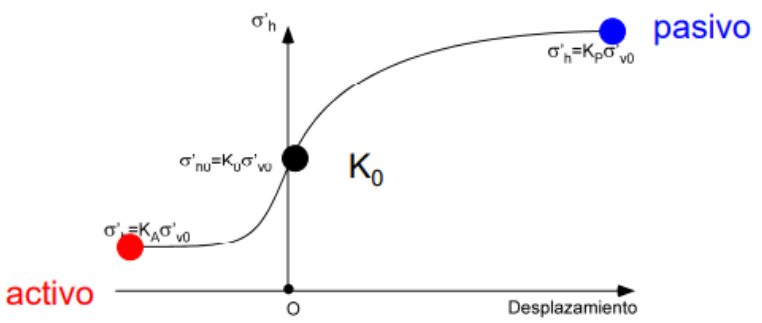
\includegraphics[width=0.5\textwidth]{img/im4}
		\caption{caption}
		\label{fig:label}
	\end{figure}

}

\question{¿ Puede darse el caso de que Coulomb prediga unas condiciones más desfavorables que Rankine en el caso activo ?}{
	No, ya que al considerar el rozamiento parte del empuje es estabilizador.
}

\question{ Hipótesis y utilización de la fórmula de Rankine }{
	\begin{enumerate}
		\item Todo el suelo esta en rotura
		\item La superficie de rotura es plana
		\item Rozamiento suelo/muro es nulo $\Rightarrow$ Tensiones principales
	\end{enumerate}
	Uso:
	\begin{enumerate}
		\item Trasdós vertical
		\item Terreno horizontal o inclinado un ángulo $\beta$
	\end{enumerate}
}

\question{Hipótesis de Coulomb para la determinación del empuje activo}{
	\begin{enumerate}
		\item Rotura plana: las lineas de contorno están en rotura 
		\item ``Suelo no cohesivo (c’=0) $\rightarrow$ friccional''
		\item ``No existen cargas aplicadas en superficie''
		\item Suelo homogéneo
		\item Suelo isotropo
		\item ``No hay agua $\rightarrow$ suelo seco''
	\end{enumerate}
}

\question{ En que casos se puede utilizar la teoría de Coulomb para la determinación del empuje pasivo ? Razonar}{
	Coulomb sobre-valora el empuje pasivo al considerar el rozamiento. Supone roturas planas cuando en realidad son curvas. Cúanto mayor sea $\delta$ mayor la distancia con la realidad.
}


% section questions (end)

\newpage

\section{Estructuras de contención} % (fold)
\label{sec:estructuras_de_contención}

\subsection{Muros de gravedad} % (fold)
\label{sub:muros_de_gravedad}

\begin{mydef}[Regla del núcleo central]
	Corresponde a la condición de no existencia de tracciones (suponiendo una distribución lineal). No es restristictiva se puede prescindir de ella en casos de terrenos duros (arcillas duras, rocas…). Ocurre si el punto de aplicación de la resultante respecto la base es :
	\[
		e> \frac{B}{6}
	\]
\end{mydef}


\subsection{Pantallas} % (fold)
\label{sub:pantallas}

\begin{mybox}{Pantallas}
	Son estructuras esbeltas, construidas con material que resiste a la tracción (acero, hormigón armado)
	\tcbsubtitle{\emph{Tablestacas}}

	\begin{minipage}[t]{0.5\textwidth}
	Ventajas:
	\begin{enumerate}
		\item Flexibles
		\item Estancas
		\item Reutilización fácil
	\end{enumerate}
	\end{minipage}%
	\begin{minipage}[t]{0.5\textwidth}
	Inconvenientes:
		\begin{itemize}
			\item Limitación de longitud
			\item Corrosión
			\item Difíciles de soldar
			\item No se pueden instalar en cualquier terreno
		\end{itemize}
	\end{minipage}

	\tcbsubtitle{\emph{Hormigonadas ``in-situ''}}
	Problemas comunes:
	\begin{itemize}
		\item Fallos de hormigonado (mala colocación)
		\item Fallos de inyección (falta adherencia)
		\item Mala calidad de los materiales
	\end{itemize}

	\tcbsubtitle{\emph{Otros tipos de pantallas}}
	\begin{itemize}
		\item Pilotes
		\item Micro-pilotes
		\item Damas
		\item Entibaciones
	\end{itemize}

	\tcbsubtitle{\emph{Posibles modos de fallo}}

	\tcbsubtitle{\emph{Estado tensional en voladizo}}

	\begin{minipage}[t]{0.5\textwidth}
	\begin{figure}[H]
		\centering
		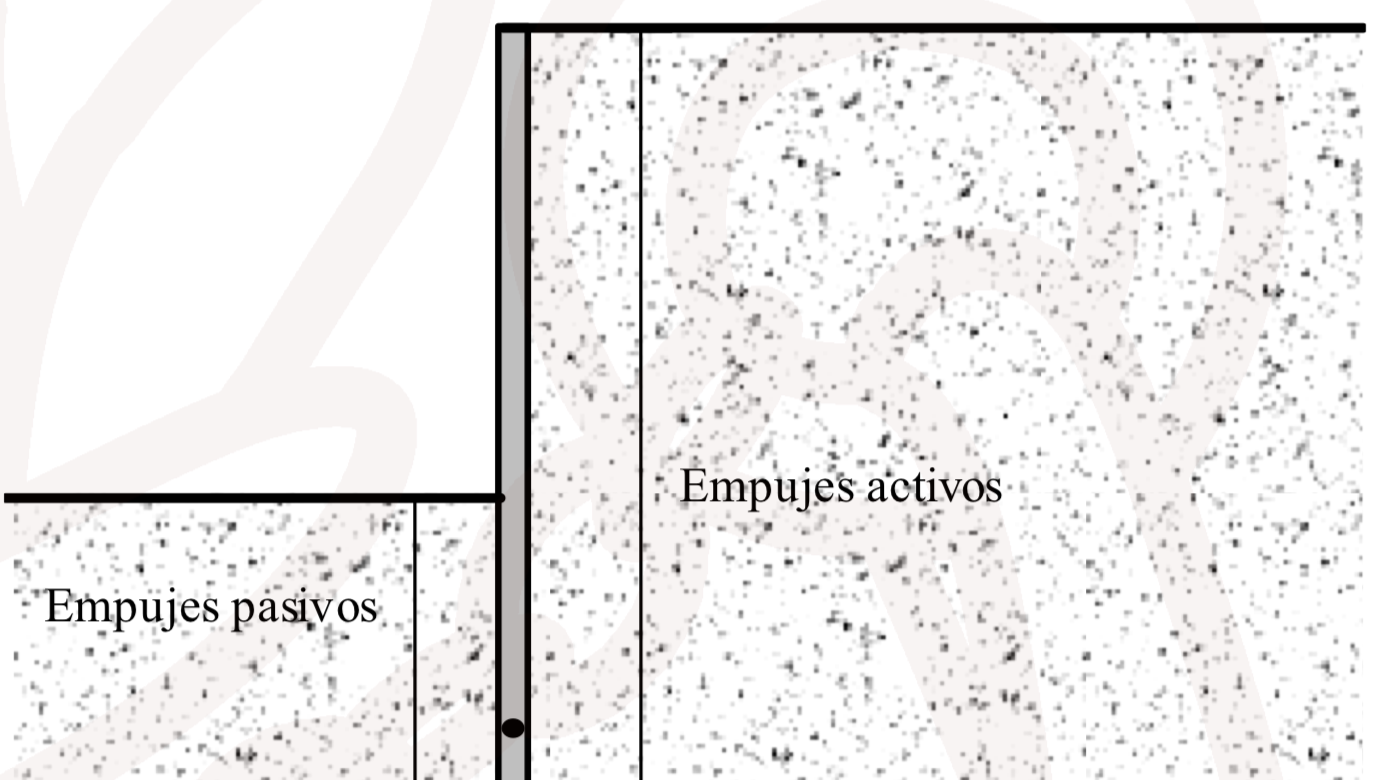
\includegraphics[width=0.95\textwidth]{img/confi1}
		\caption{Estado tensional 1 (translación)}
		\label{fig:confi1}
	\end{figure}
	\end{minipage}%
	\begin{minipage}[t]{0.5\textwidth}
	\begin{figure}[H]
		\centering
		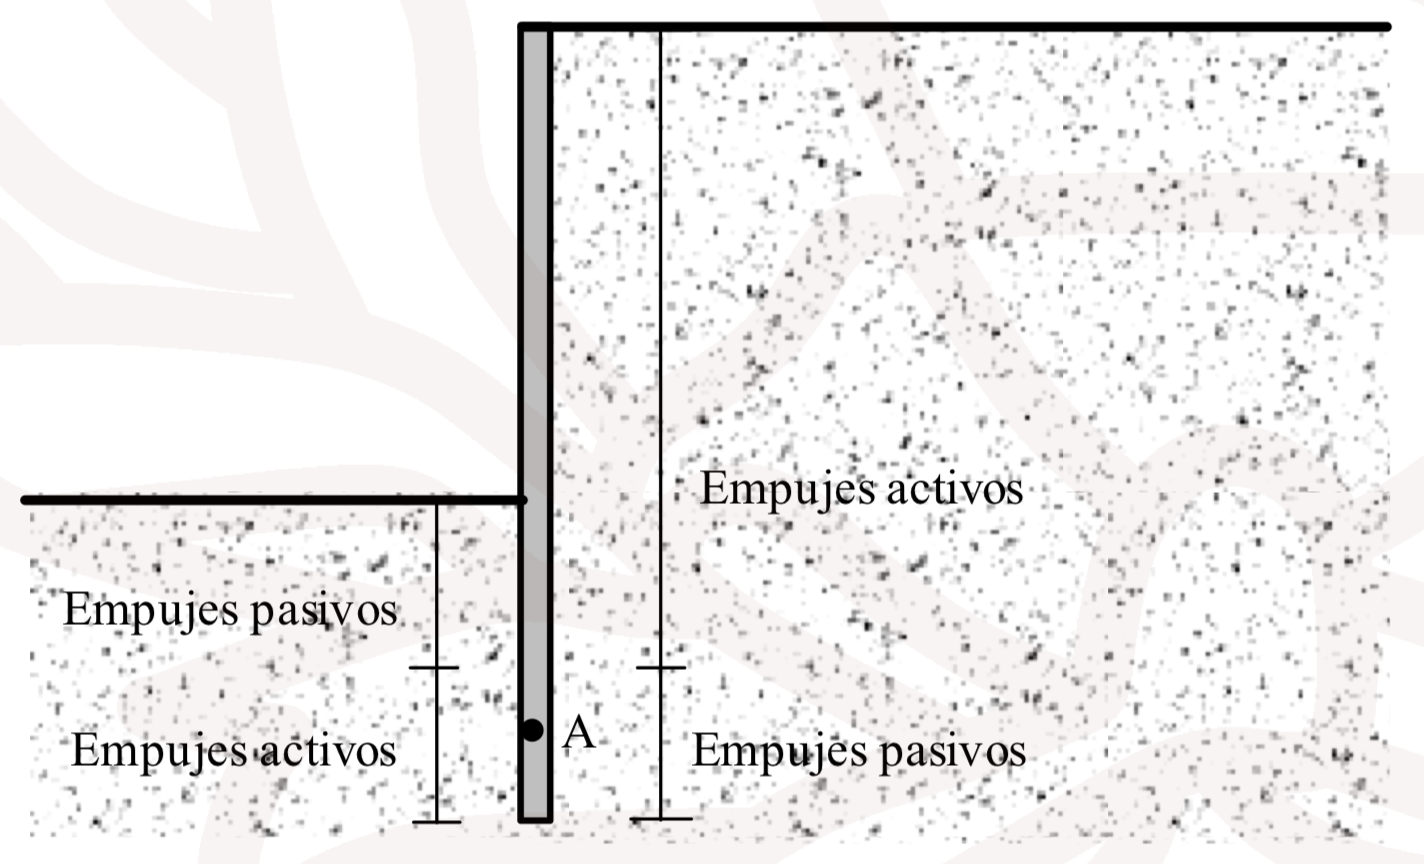
\includegraphics[width=0.95\textwidth]{img/confi2}
		\caption{Estado tensional 2 (rotación)}
		\label{fig:confi2}
	\end{figure}
	\end{minipage}

	\tcbsubtitle{\emph{Métodos de análisis}}

	\paragraph{En voladizo} % (fold)
	\label{par:en_voladizo}

	Sólo podemos analizar el caso de la Figure~\ref{fig:confi2} ya que la Figure~\ref{fig:confi1} no es estable.
	
	\begin{figure}[H]
		\centering
		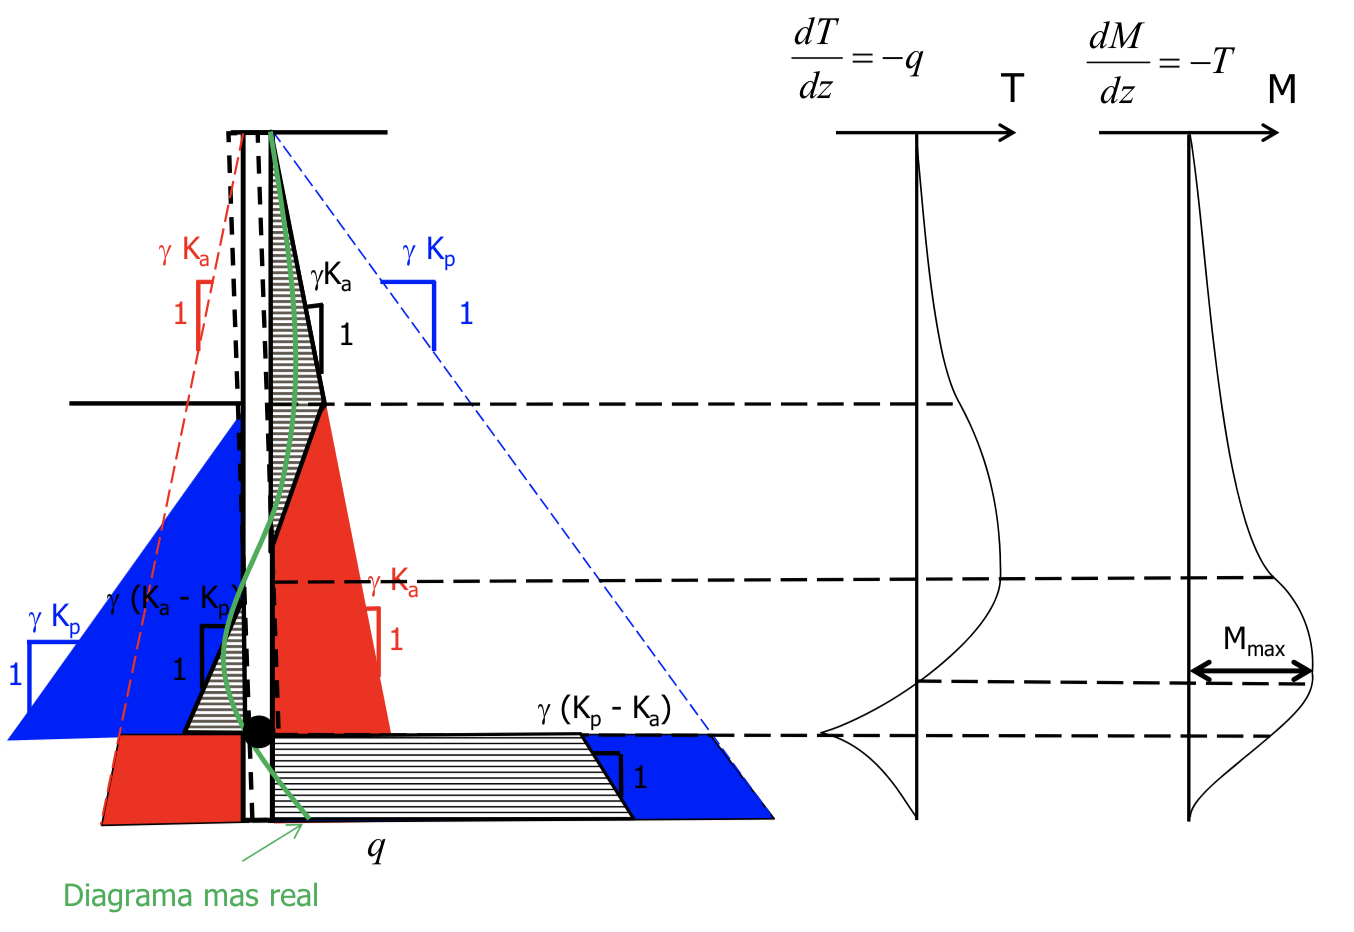
\includegraphics[width=0.95\textwidth]{img/voladizo}
		\caption{Análisis voladizo}
		\label{fig:voladizo}
	\end{figure}
	% paragraph en_voladizo (end)

	\paragraph{Soporte libre} % (fold)
	\label{par:soporte_libre}
	El estado tensional es cómo Figure~\ref{fig:confi1}. Este método considera que la profundidad del empotramiento es pequeña o que la rigidez de la pantalla es grande. Se asume que la pantalla se desplaza de una manera rígida bajo el efecto de la \emph{presión activa} de tierras y moviliza la presión pasiva a lo largo de su parte empotrada. Se considera que no hay reacción en la base. Es un sistema isostático no necesitamos hipótesis adicionales.
	\begin{figure}[H]
		\centering
		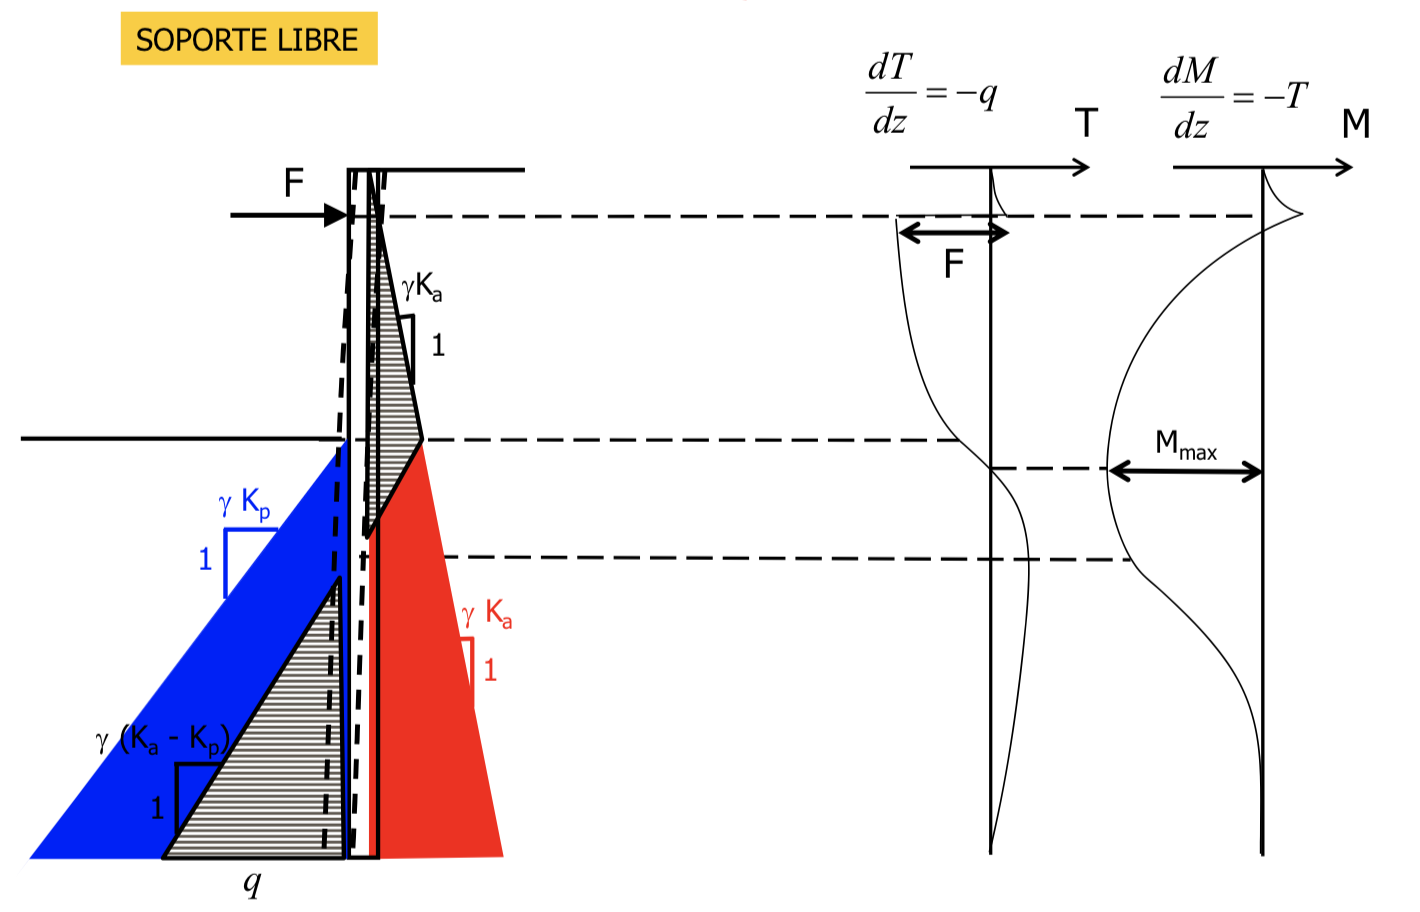
\includegraphics[width=0.95\textwidth]{img/soporte_libre}
		\caption{Análisis soporte libre}
		\label{fig:soporte_libre}
	\end{figure}
	% paragraph soporte_libre (end)

	\paragraph{Soporte fijo} % (fold)
	\label{par:soporte_fijo}
	El estado tensional es cómo la Figure~\ref{fig:confi2}. Este método considera que la rigidez es pequeña o la profundidad del empotramiento grande. Se considera que la base está empotrada. Este sistema es hiperestático, así pues es necesario realizar la hipótesis siguiente para resolverlo.
	\[
		x | \ q=0 \Leftrightarrow T(x) = T_{max} := M(x)=0
	\]
	\begin{figure}[H]
		\centering
		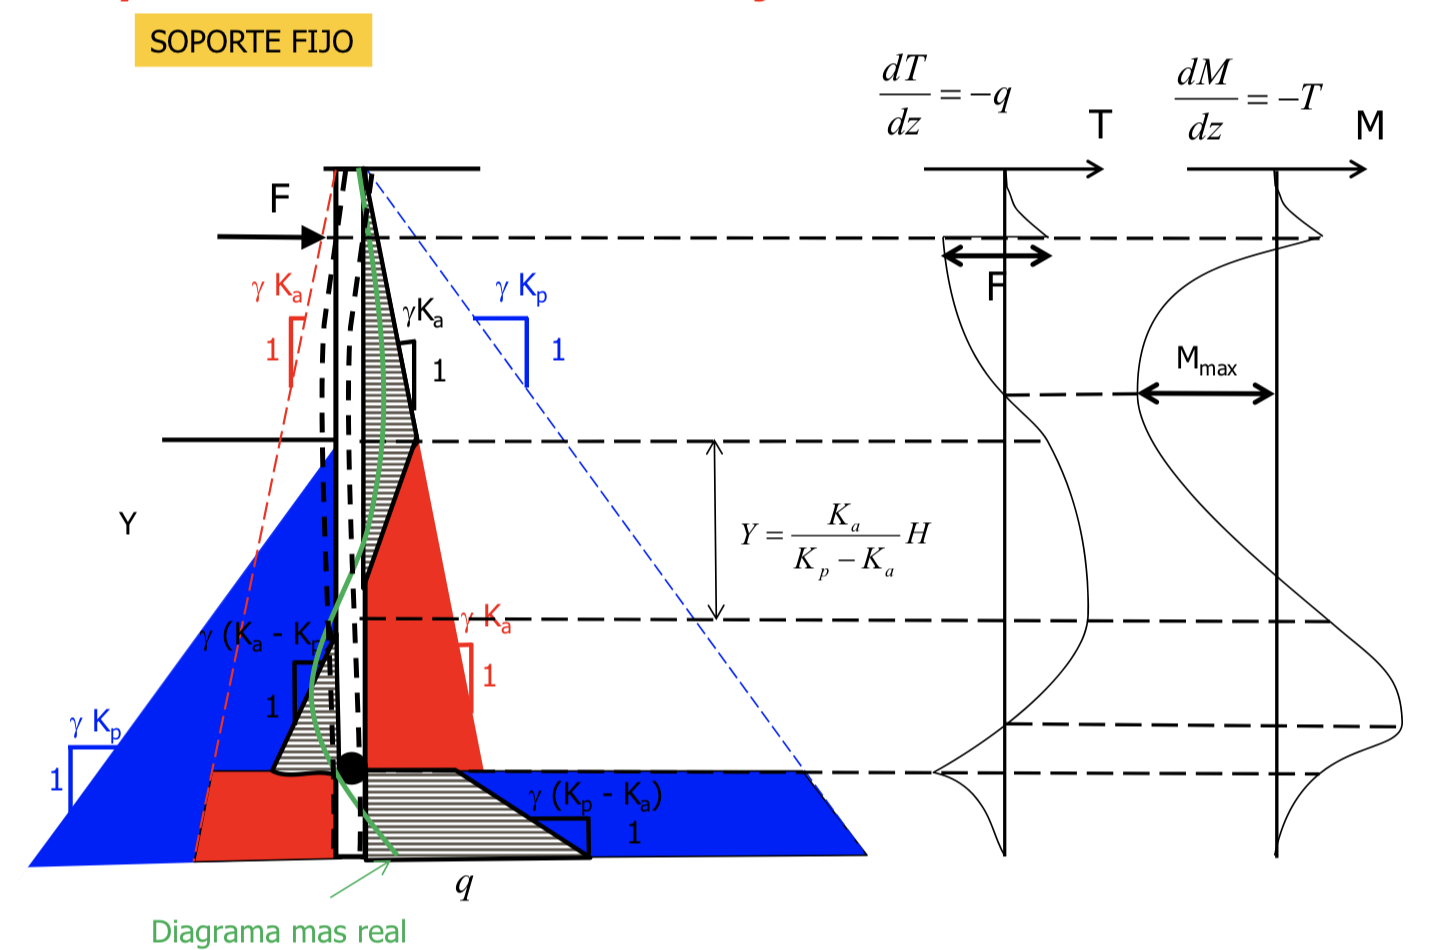
\includegraphics[width=0.95\textwidth]{img/soporte_fijo}
		\caption{Análisis soporte fijo}
		\label{fig:soporte_fijo}
	\end{figure}
	% paragraph soporte_fijo (end)
\end{mybox}

\begin{mybox}{Tierra reforzada}
	No requieren cimentación, tienen un buen comportamiento en suelos de mala calidad y permiten alturas importantes ($h>20m$)
	\begin{minipage}[t]{0.5\textwidth}
	Ventajas:
	\begin{enumerate}
		\item Estructura flexible (se adapta a asientos importantes en cimentación)
		\item Ejecución rápida con material ligero
		\item Coste competitivo
		\item Se pueden alcanzar alturas importantes
	\end{enumerate}
	\end{minipage}%
	\begin{minipage}[t]{0.5\textwidth}
	Inconvenientes:
		\begin{itemize}
			\item Relleno debe ser de calidad
			\item Problemas de durabilidad (corrosión de armaduras)
		\end{itemize}
	\end{minipage}
	\tcbsubtitle{\emph{Posibles modos de fallo}}

	\begin{enumerate}
		\item Por rotura a tracción de la armadura
		\item Por falta de adherencia armadura-relleno en la zona resistente
	\end{enumerate}

	\tcbsubtitle{\emph{Condiciones de estabilidad}}
	\begin{enumerate}
		\item Rotura a tracción:
		\[
			T_M \leq \frac{1}{F_1}\sigma_r b e
		\]
		\item Adherencia:
		\[
			T_M^{*}\leq \frac{1}{F_2}\int_0^{2a}\mu^* \sigma_v(x)2bdx
		\]

	\end{enumerate}
	Cálculo de la tracción máxima:
	\[
		T_M = \frac{1}{n}\sigma_h \Delta H
	\]
\end{mybox}

% subsection pantallas (end)
% subsection muros_de_gravedad (end)
% section estructuras_de_contención (end)

\newpage

\part{Questions} % (fold)
\label{prt:questions}

% part questions_ (end)

\question{Cómo puedes determinar el valor de la resistencia al corte sin drenaje ($C_u$) de una arcilla a partir de un ensayo de compresión simple ? ¿ Qué fiabilidad te merece el resultado ?}{
	\begin{figure}[H]
			\centering
			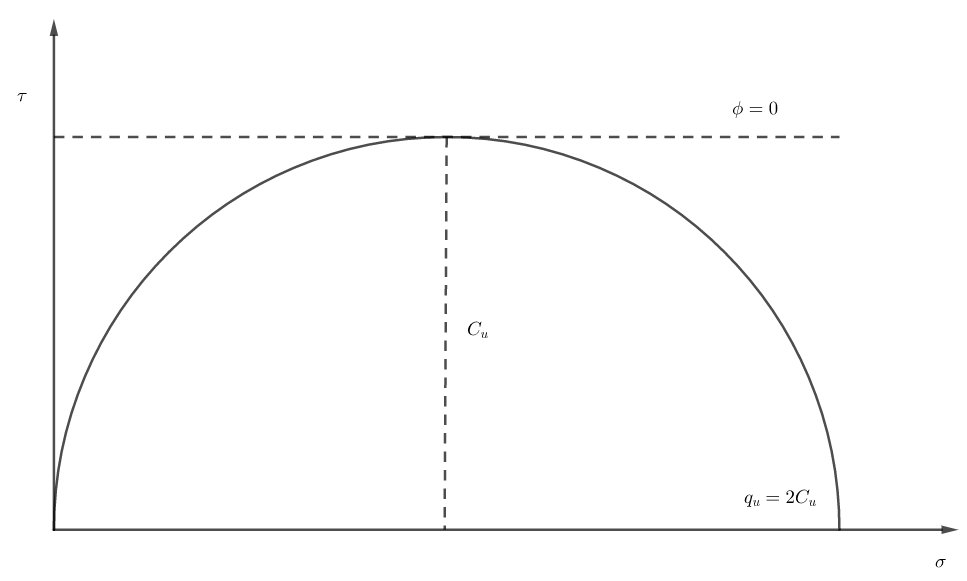
\includegraphics[width=0.5\textwidth]{img/cu}
			\caption{Circulo de Mohr: compresión simple sin drenaje}
			\label{fig:cu}
	\end{figure}
	Se rompen distintas provetas y se encuentra la envolvente de rotura. La fiabilidad del resultado dependerá del la alteración de la muestra.
}

\question{Cúando se utilizan los resultados del ensayo del molinete (vane-test) para estimar el valor de $C_u$ de una arcilla, se suele aplicar un factor de corrección que depende del índice de plasticidad del suelo. ¿ A qué se debe la necesidad de esta corrección? ¿ A partir de qué datos se ha determinado dicho factor?}{
	Se aplica por:
	\begin{itemize}
		\item Anisotropia del terreno
		\item Velocidad de cargo (más rapida que en campo)
	\end{itemize}
	Aplicamos un factor de corrección que varia en función del indice de plasticidad (IP), véase Figure~\ref{fig:mu}
	\begin{figure}[H]
			\centering
			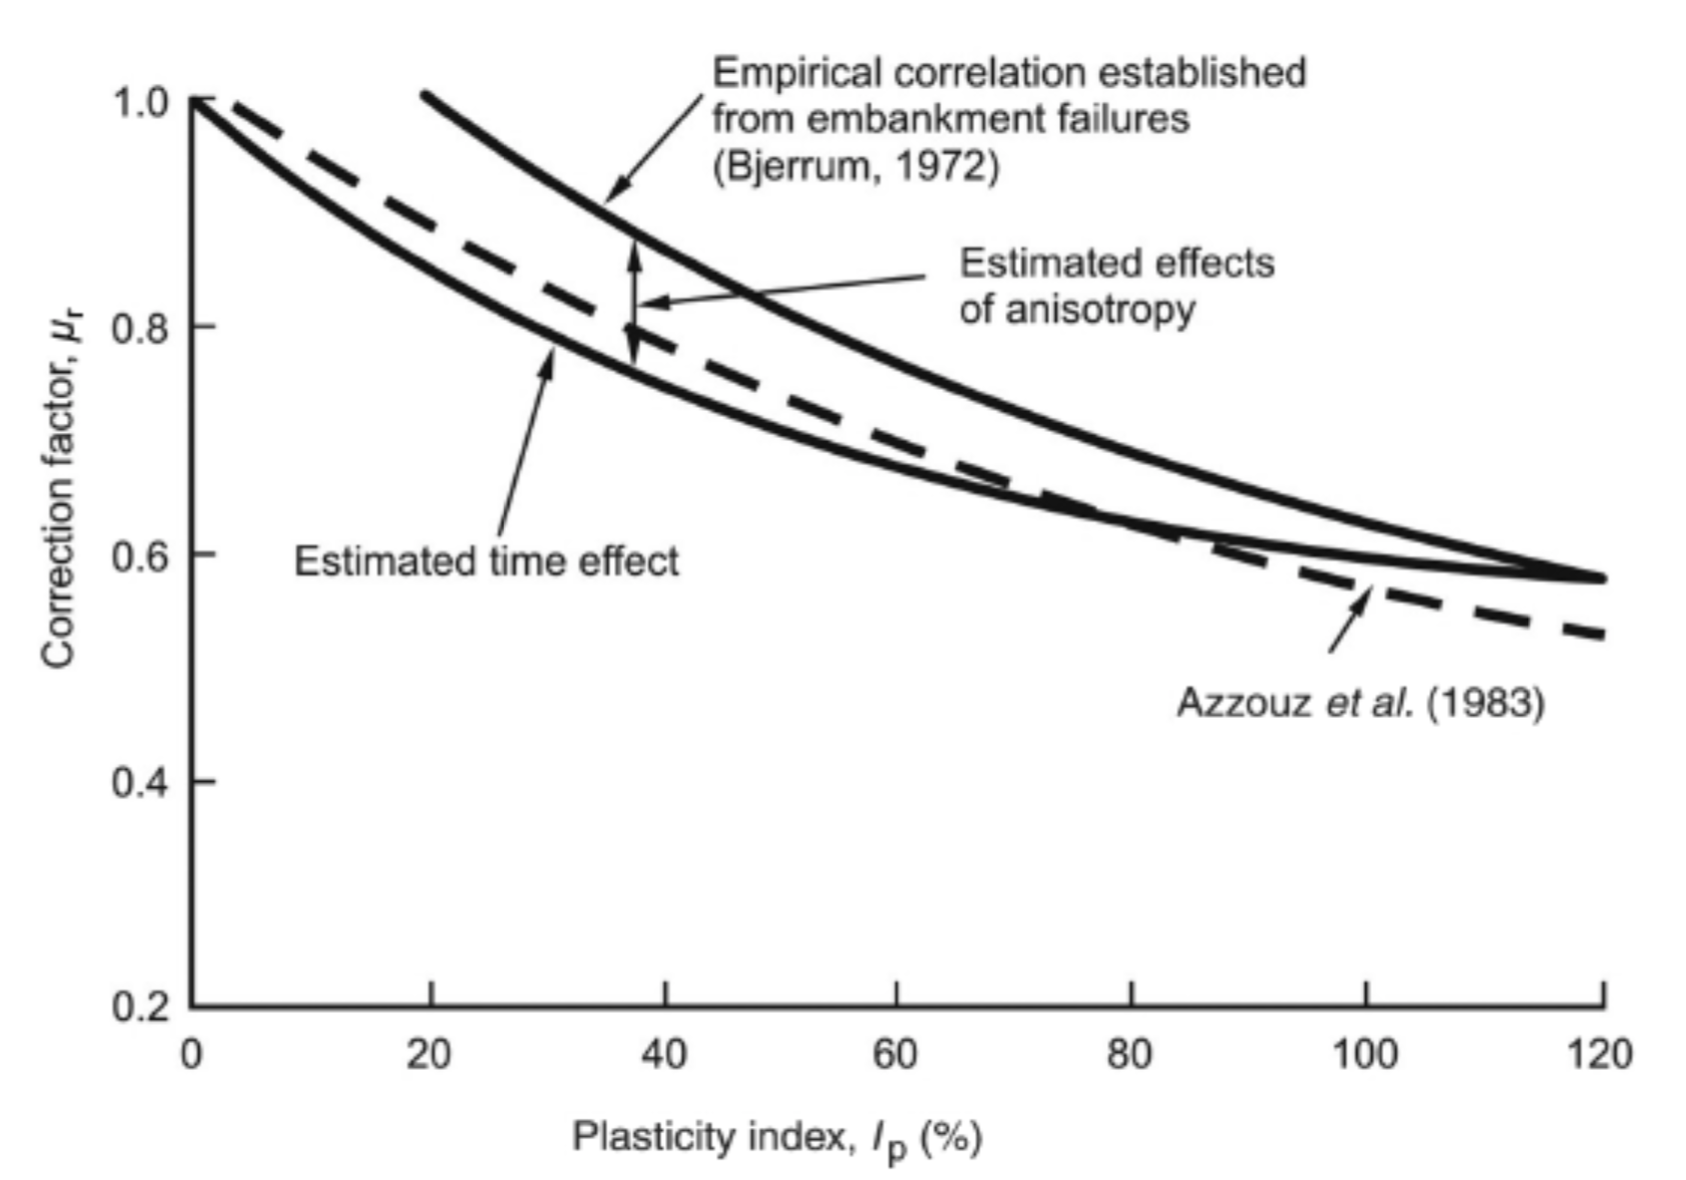
\includegraphics[width=0.5\textwidth]{img/mu}
			\caption{Factor de corrección Vane test}
			\label{fig:mu}
	\end{figure}
}

\question{Suponiendo que una arcilla se comporta con un modelo eláso-perfectamento plástico, dibujar la evolución de la presión intersticial que se medirá en un ensayo presiométrico (se considera condiciones no drenadas).}{
	\begin{figure}[H]
			\centering
			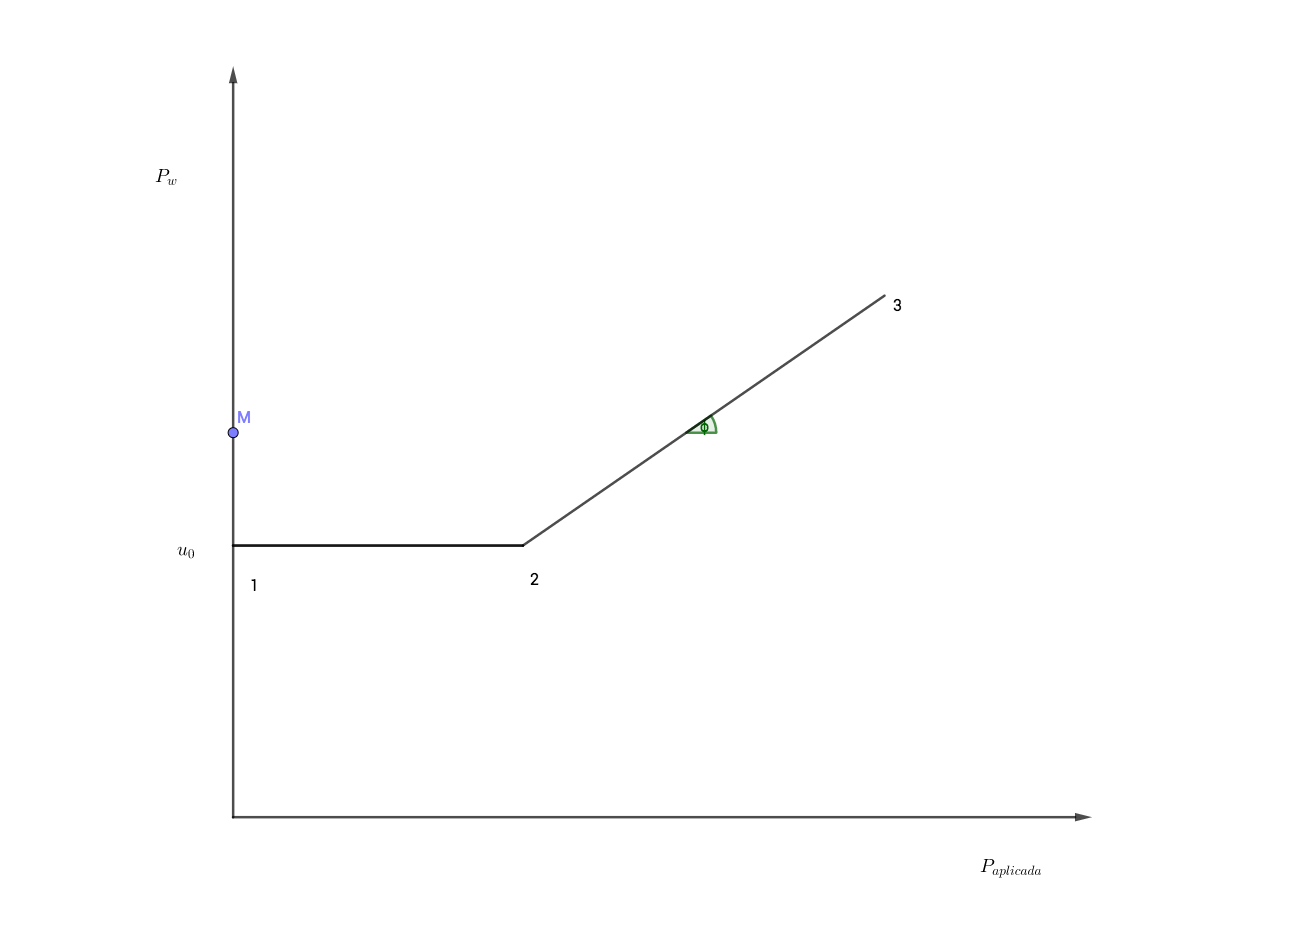
\includegraphics[width=0.5\textwidth]{img/u_evolution}
			\caption{Evolución de la presión intersticial}
			\label{fig:mu}
	\end{figure}
	Véase la evolución de los circulos de mohr en las Figure~\ref{fig:presio1},\ref{fig:presio2},\ref{fig:presio3}

	\begin{minipage}{0.5\linewidth}
		\begin{figure}[H]
		\centering
		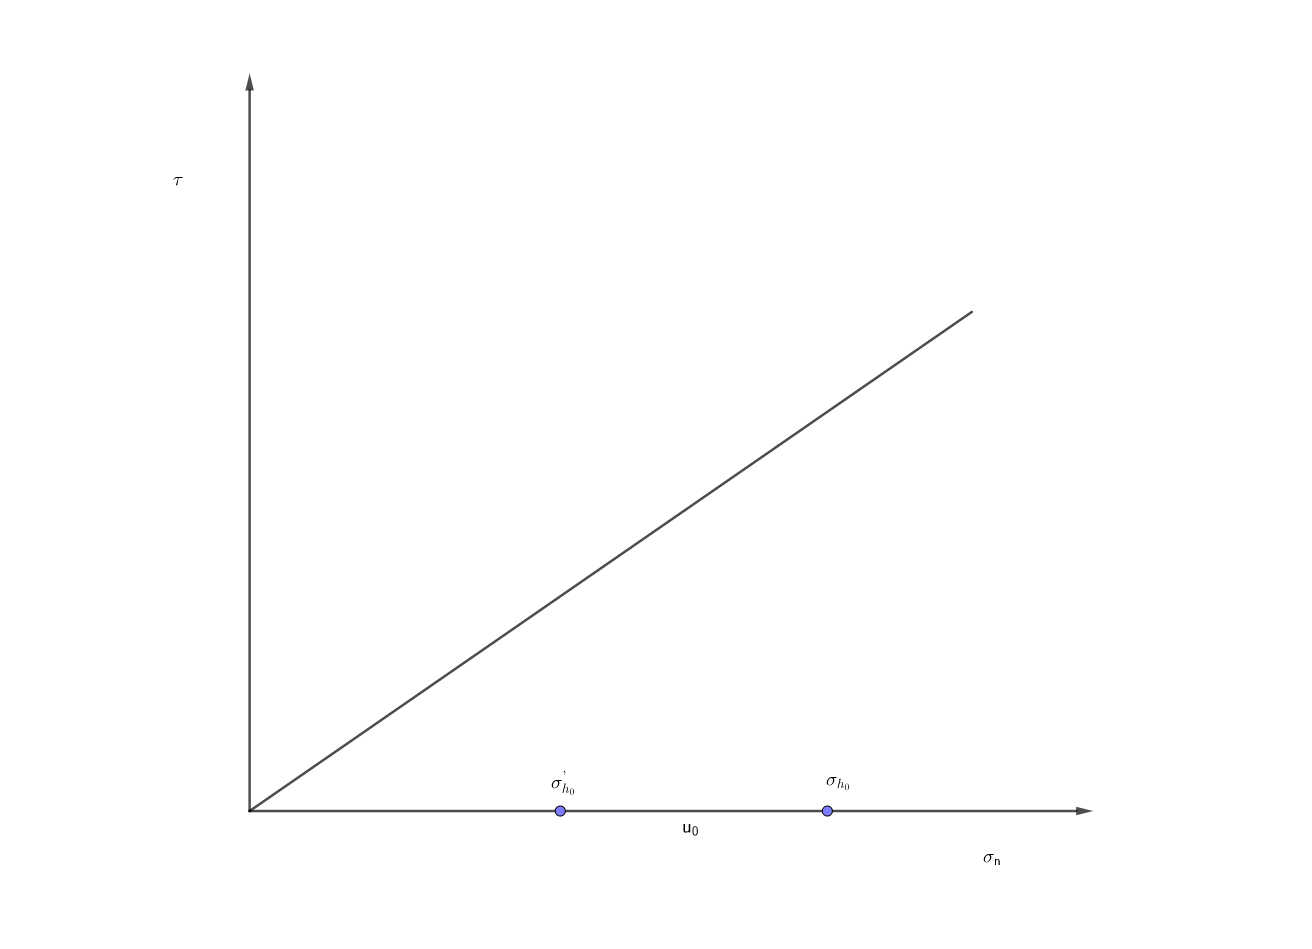
\includegraphics[width=\textwidth]{img/presio1}
		\caption{Estado inicial}
		\label{fig:presio1}
		\end{figure}
	\end{minipage}%
	\begin{minipage}{0.5\linewidth}
		\begin{figure}[H]
			\centering
			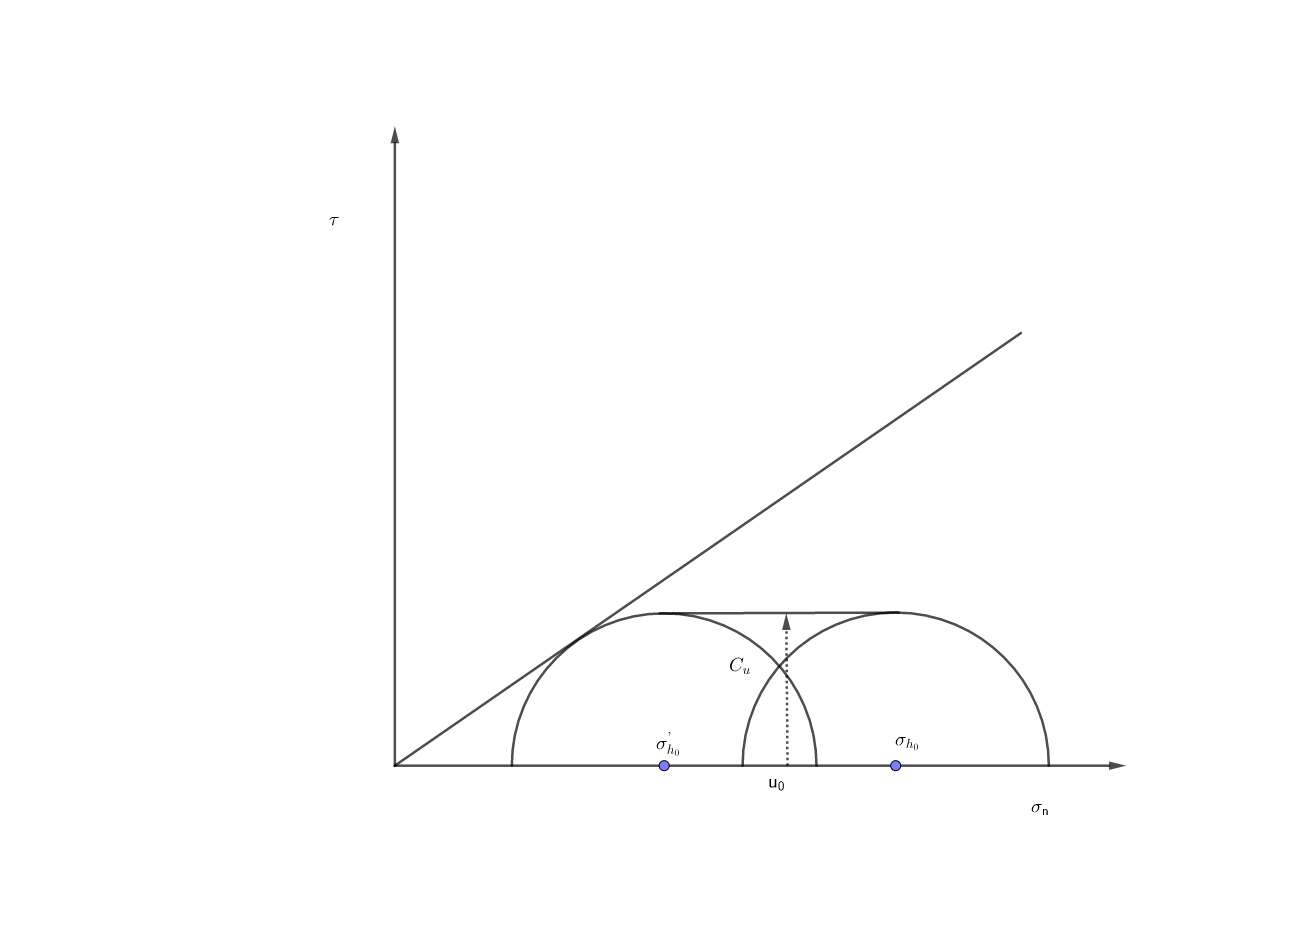
\includegraphics[width=\textwidth]{img/presio2}
			\caption{Incremento de presión con presión intersticial constante}
			\label{fig:presio2}
		\end{figure}
	\end{minipage}
	\begin{figure}[H]
			\centering
			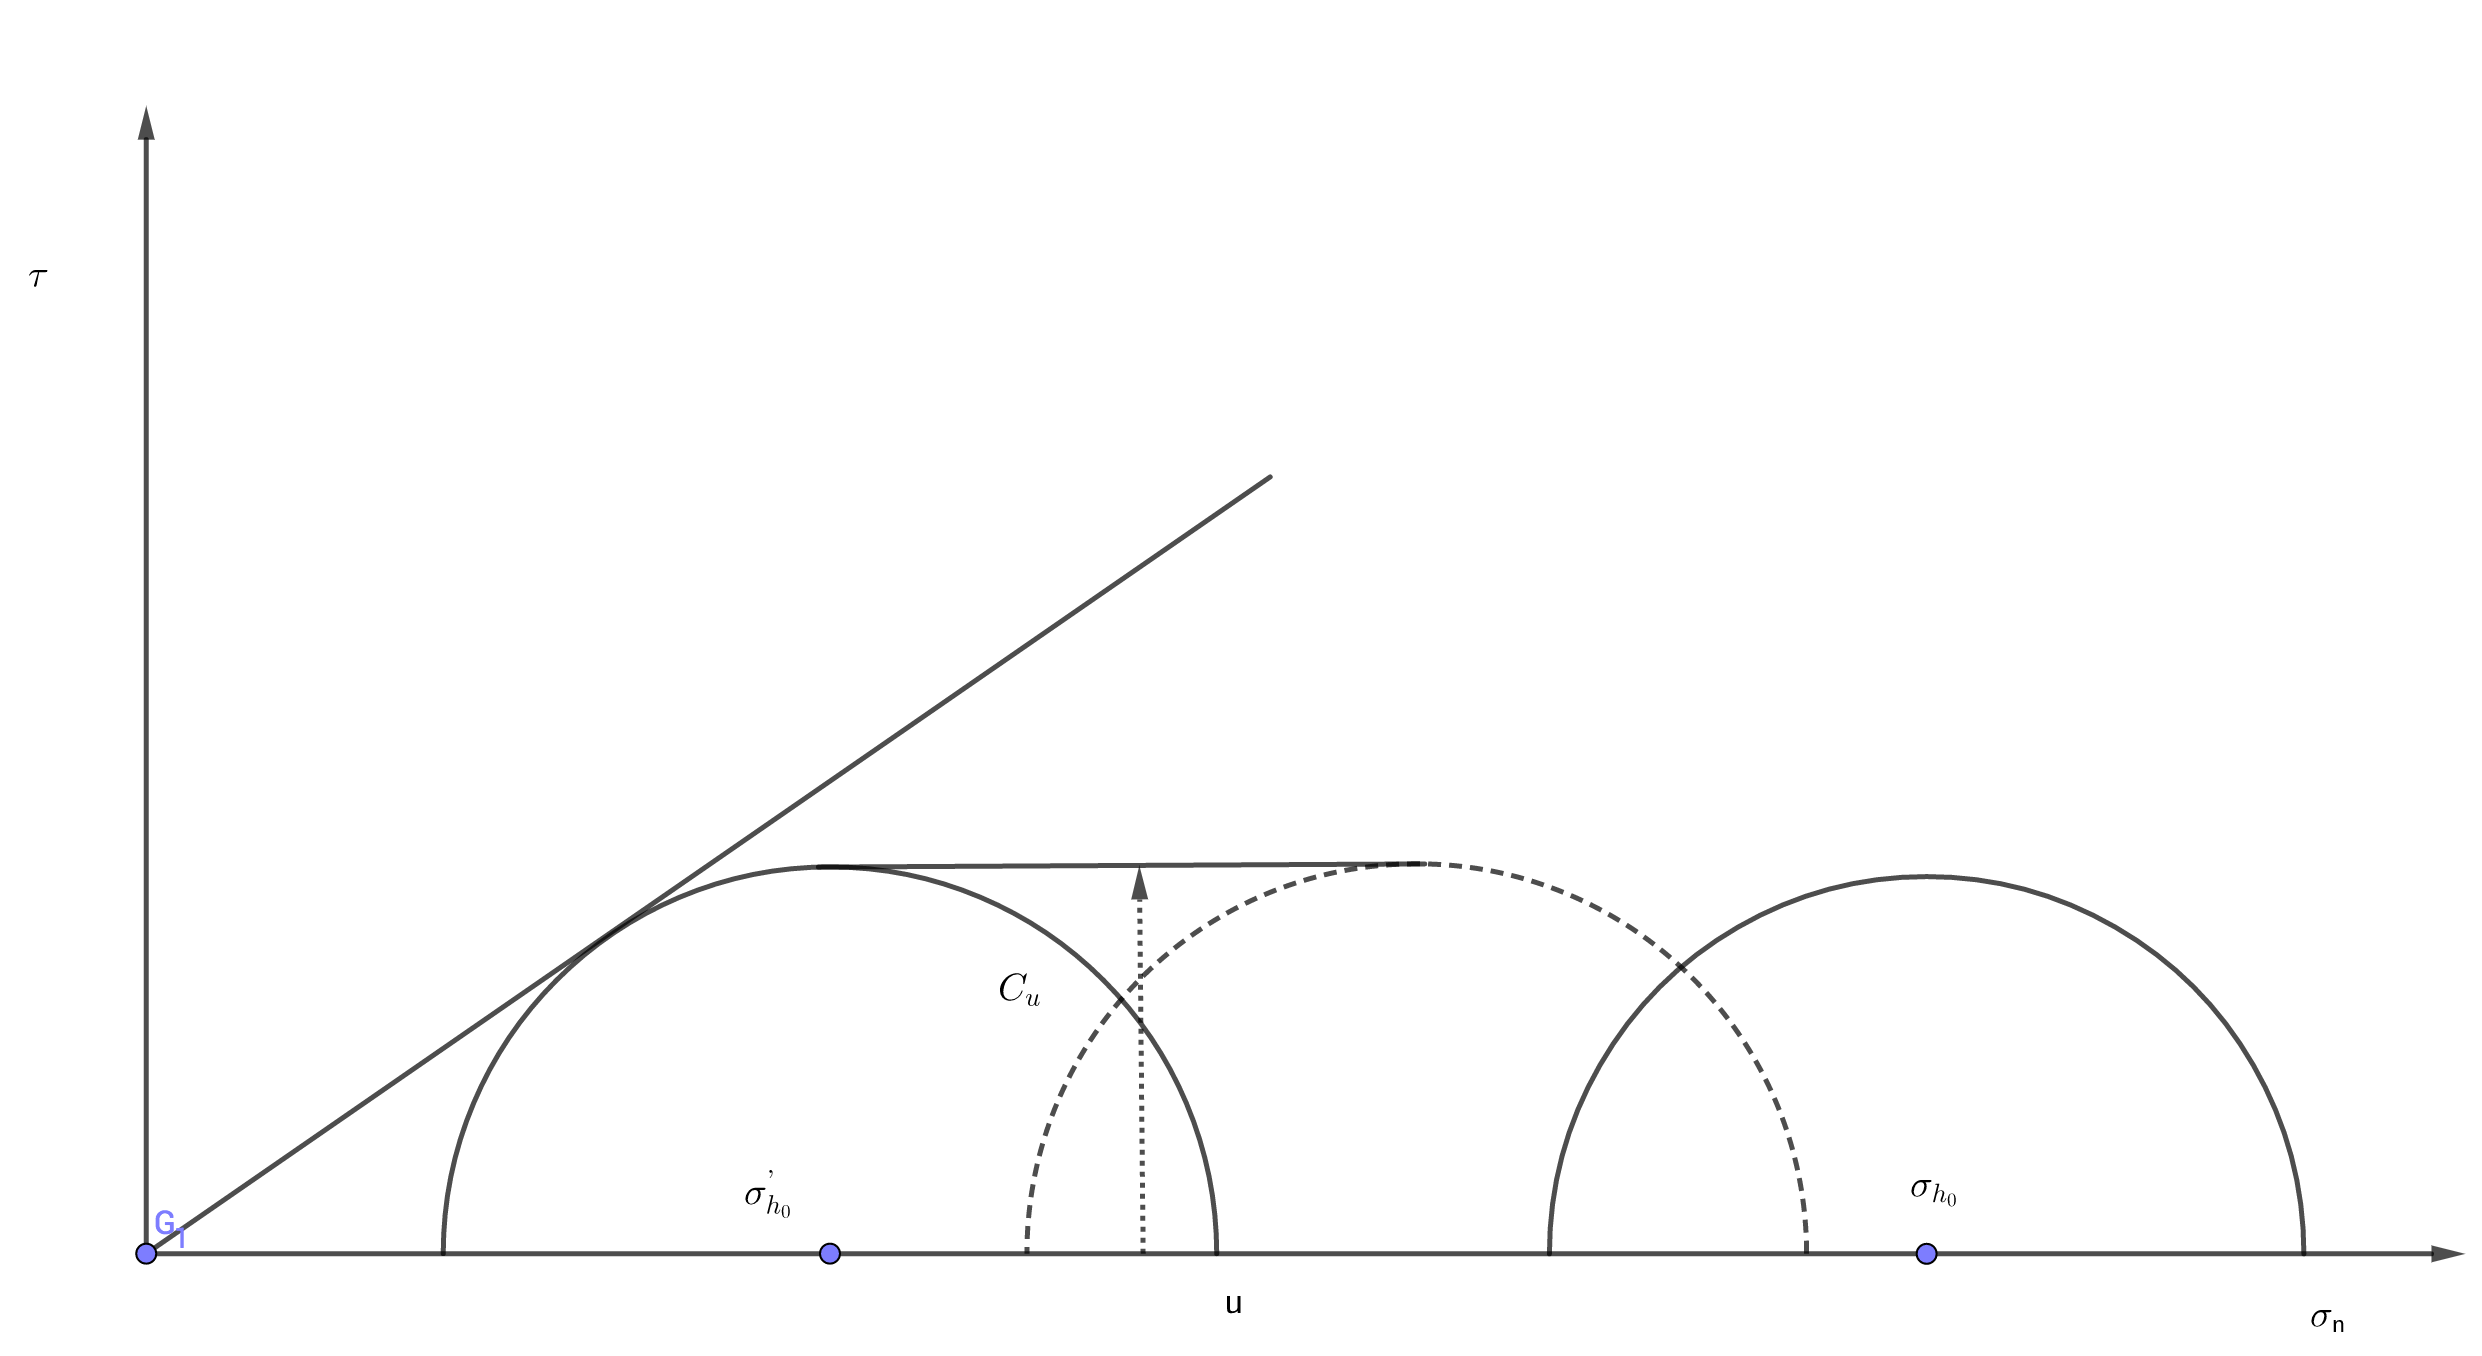
\includegraphics[width=0.6\textwidth]{img/presio3}
			\caption{Aumento de la presión intersticial}
			\label{fig:presio3}
	\end{figure}
}


% section questions (end)

\newpage

\section{Cimentaciones superficiales} % (fold)
\label{sec:parte_2}


\question{Indica las principales hipotésis del método edométrico para el cálculo de asientos de consolidación y describe brevemente su grado de validez.}{
	Hipótesis:
	\begin{enumerate}
		\item Cálculo de $\sigma_v$ por elasticidad.
		\item $\Delta u = \Delta \sigma_v = \Delta \sigma_v^{’}$, el aumento de presión interna es igual al aumente de presión vertical.
		\item Las tensiones totales se mantienen invariantes a lo largo de la consolidación.
	\end{enumerate}
	Es válido (muy usado) aunque la segunda hipótesis se distancia de la realidad.
	\begin{myrem}[Skempton-Bjerrum]
		Intenta mejorar el efecto de la segunda hipótesis.
	\end{myrem}
}


\question{Calcular FS de la cimentación cuadrada de la Figure~\ref{fig:cimen} en condiciones no drenadas utilizando carga neta. Comenta el resultado.}{
	Al estar en situación no drenada tenemos:
	\[
		q_r = C_u N_c + q
	\]
	\begin{figure}[H]
		\centering
		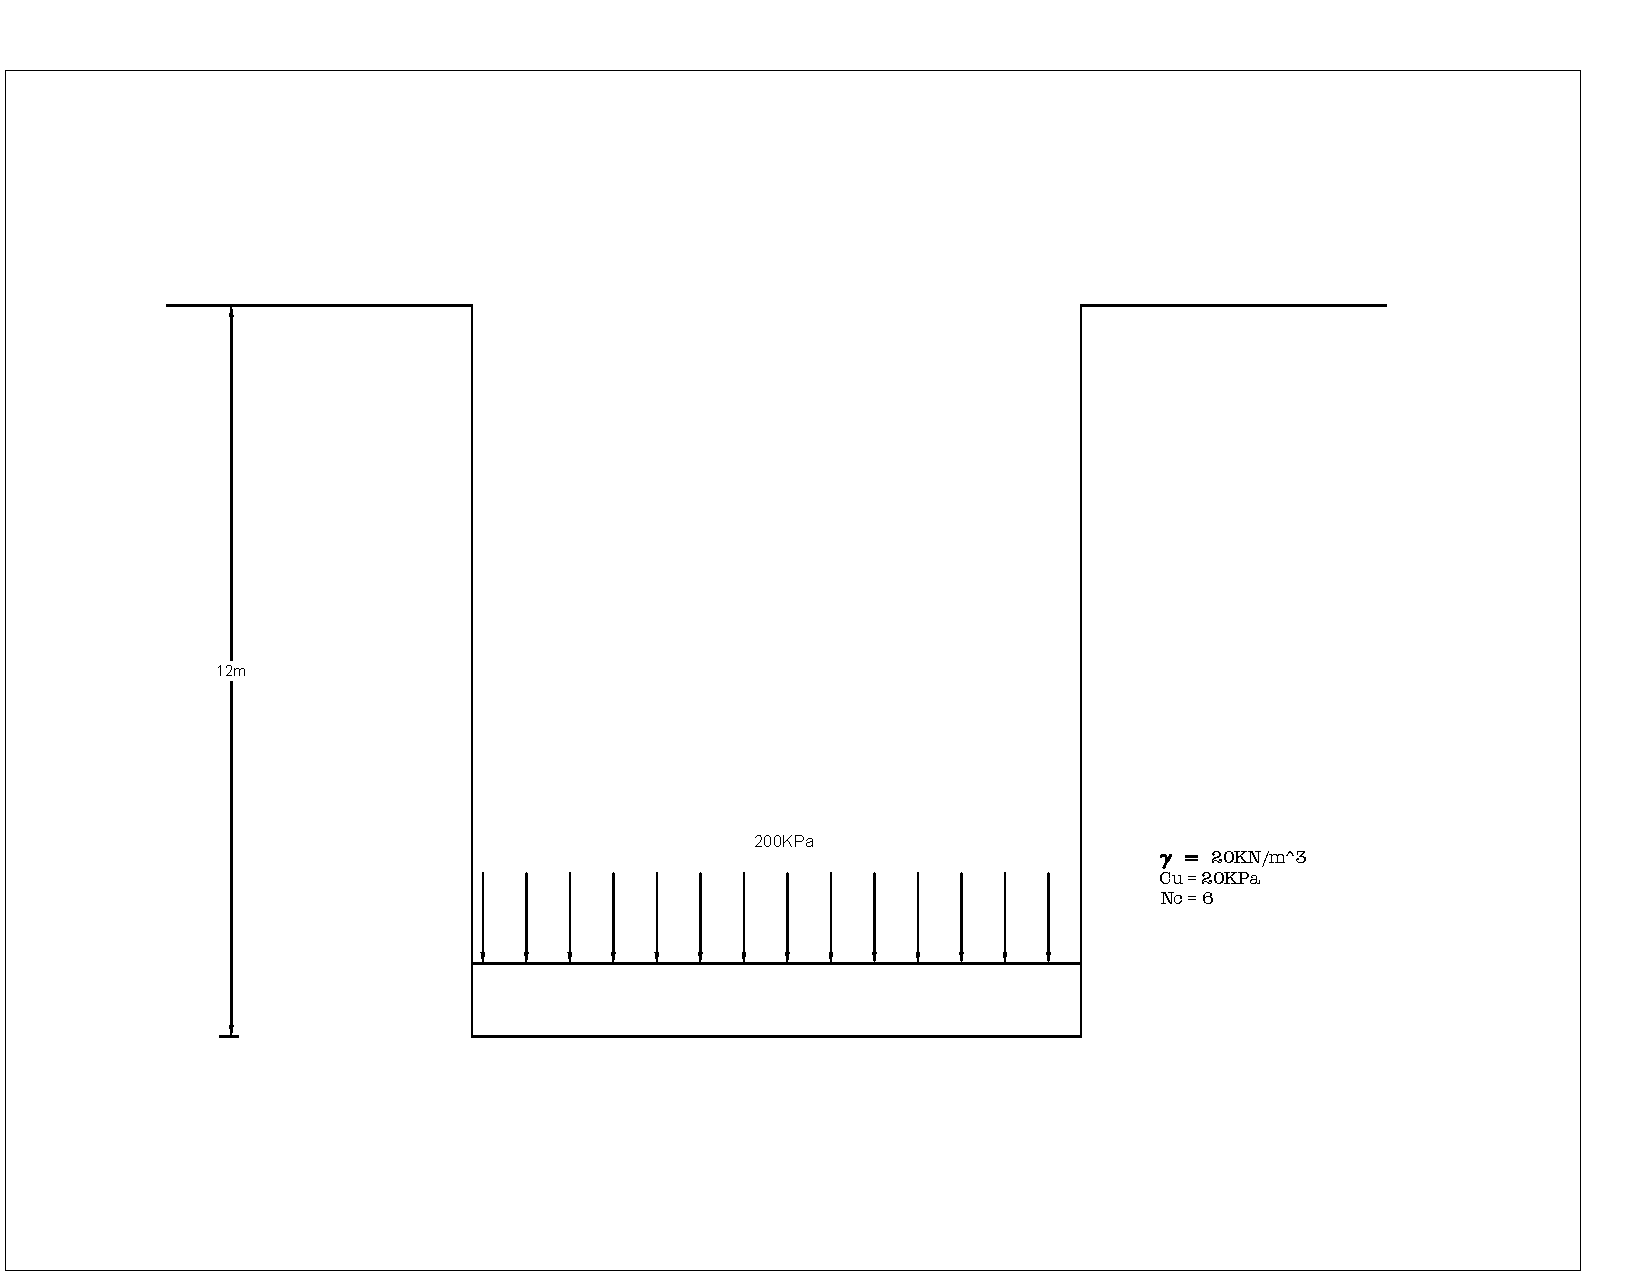
\includegraphics[width=0.9\textwidth]{img/capacidad_portante}
		\caption{Cimentación cuadrada}
		\label{fig:cimen}
	\end{figure}

	Tenemos (aplicando carga neta):
	\[
		FS = \frac{q_r - q}{q_{ad}-q} = \frac{360-240}{200 - 240} <0
	\]


	Lo cual es lógico ya que si analizamos la carga que este terreno soportaba antes de excavar observamos que era superior. Luego no hay razón de dudar de la estabilidad de esta cimentación.

	\begin{myrem}[FS real]
		Al calcular sin carga neta obtenemos
		\[
			FS = \frac{q_r }{q_{ad}} = \frac{360}{200} \approx 1,8
		\]
		Lo cual es incoherente con lo previamente comentado.
	\end{myrem}
}



\question{El asiento de una placa circular rígida sobre un semiespacio elástico homogéneo se expresa como $s=\frac{1-\mu^2}{2}\frac{P}{aE}$, donde s es el asiento, P la carga total aplicada, a el radio de la placa, E el módulo de elasticidad y $\mu$ el coeficiente de Poisson. Determinar la expresión para el módulo de balasto en estas condiciones. Comentar brevemente lo más destacado del resultado.}{
El módulo de balasto no es un parámetro del terreno. El módulo de balasto se puede determinar a partir de E,$\mu$ del terreno para una geometría dada. En este caso el el módulo de balasto variará en función del radio a.
	\[
		K = \frac{P}{s} = \frac{2aE}{1-\mu^2}
	\]
}

\question{La Figure~\ref{fig:ciment_larga} representa la cimentación cuadrada (6x6m) de una pila (circular de 2m de $\phi$) de un puente situado en un embalse. La cimentación alcanzaría su capacidad portante total si se aplicara una carga P de 1600T de forma rápida (condiciones no drenadas). ¿Con qué carga se alcanzaría la capacidad portante si el nivel del embalse estuviera 6m por encima del actual.}{
	\begin{figure}[H]
		\centering
		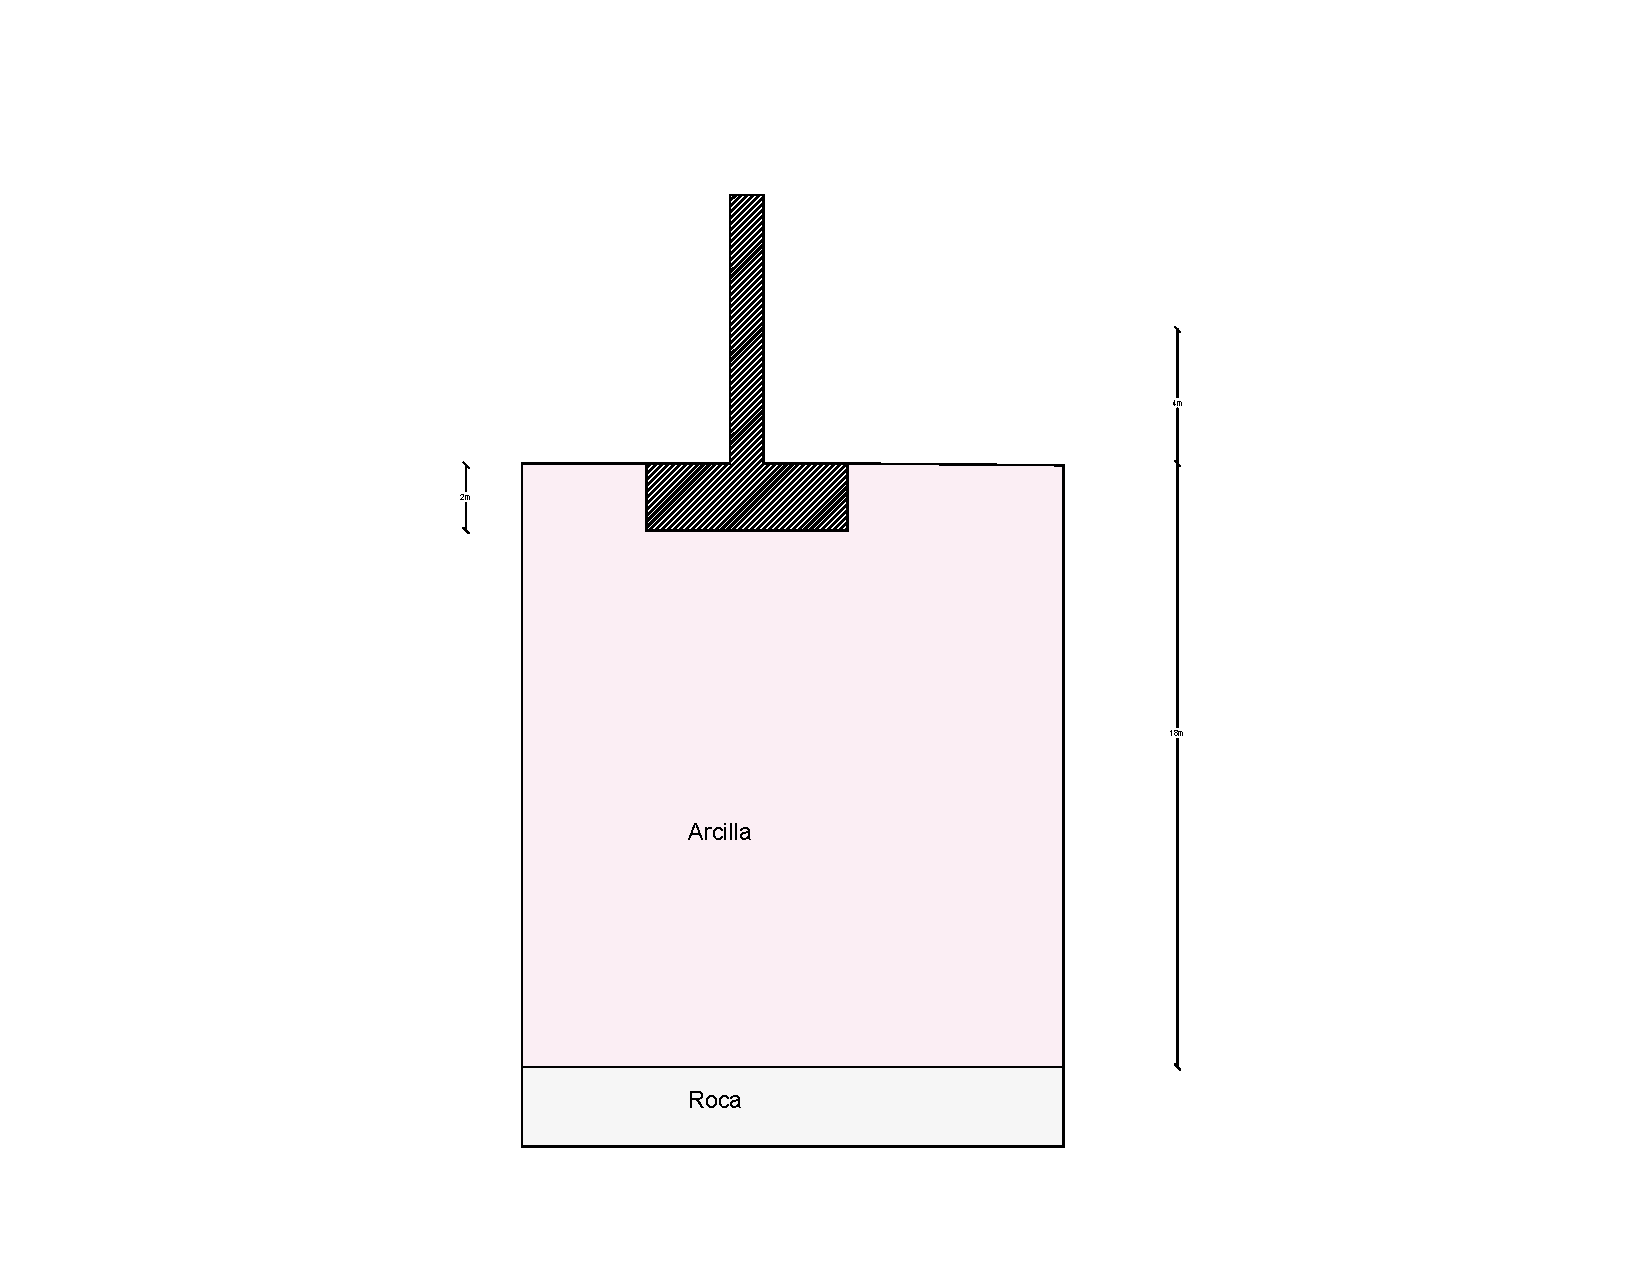
\includegraphics[width=0.5\textwidth]{img/cimentacion_larga}
		\caption{Cimentación cuadrada}
		\label{fig:ciment_larga}
	\end{figure}

	Al aplicarse rápidamente carga, nos situamos en condiciones drenadas. Analizaremos el problema en presiones totales y efectivas. Supondremos en ambos análisis $P = P_{peso-propio} + P_{peso aplicado}$

	\paragraph{Presiones totales} % (fold)
	\label{par:presiones_totales}
	
	\begin{multline}
		q_r = C_u N_c + \gamma_w H  = \frac{P + \gamma_w (H-h_b)(A_b - A_c)}{A_b}\\
		\Leftrightarrow P = C_u N_c A_b + \gamma_w (H- h_b) A_c + \gamma_w h_b A_b
	\end{multline}
	% paragraph presiones_totales (end)

	\paragraph{Presiones efectivas} % (fold)
	\label{par:presiones_efectivas}

	\begin{multline}
		q_r = C_u N_c  = \frac{P - \gamma_w h_b A_b - \gamma_w (H-h_b)(A_b - A_c)}{A_b}\\
		\Leftrightarrow P = C_u N_c A_b + \gamma_w (H- h_b) A_c + \gamma_w h_b A_b
	\end{multline}
	
	% paragraph presiones_efectivas (end)

	Luego tenemos 
	\[
		\Delta P = \gamma_w \Delta H A_c
	\]
}

\question{Si la carga se aplica lentamente (drenada), el valor de carga P con la que se alcanza la capacidad portante es de 12200T. ¿Con qué carga se alcanzaría la capacidad portante si el nivel del embalse estuviera 6m por encima de su nivel actual?}{
	A pesar de estar la capacidad portante en presiones efectivas, podemos trabajar en presiones totales o efectivas.
	\paragraph{Presiones totales} % (fold)
	\label{par:presiones_totales}
	\begin{multline}
		q_r^\prime + \gamma_w H = \frac{P  - \gamma_w (H-h_b)(A_b - A_c)}{A_b} \\
		\Leftrightarrow P = A_b q_r^\prime + \gamma_w H A_b  - \gamma_w (H-h_b)(A_b - A_c) \\
		\Leftrightarrow P = A_b q_r^\prime- \gamma_w H A_b h_b -  \gamma_w (H-h_b)A_c
	\end{multline}
	% paragraph presiones_efectivas (end)

	\paragraph{Presiones efectivas} % (fold)
	\label{par:presiones_efectivas}
	\begin{multline}
		q_r^\prime  = \frac{P -\gamma_w H A_b  - \gamma_w (H-h_b)A_c}{A_b} \\
		\Leftrightarrow P = A_b q_r^\prime- \gamma_w H A_b h_b -  \gamma_w (H-h_b)A_c
	\end{multline}
	% paragraph presiones_efectivas (end)

	Luego tenemos 
	\[
		\Delta P = -\gamma_w \Delta H A_c
	\]
}


\question{En el caso de la capacidad portante de una cimentación superficial ¿Qué caso es más crítico?
\begin{enumerate}
	\item Corto plazo 
	\item Largo plazo
\end{enumerate}}{
	El peor caso es a \emph{corto plazo} ya que como podemos ver en la Figure~\ref{fig:tensiones}, la trayectoria en tensiones totales (color verde) queda limitada por $C_u$. 
	\begin{figure}[H]
		\centering
		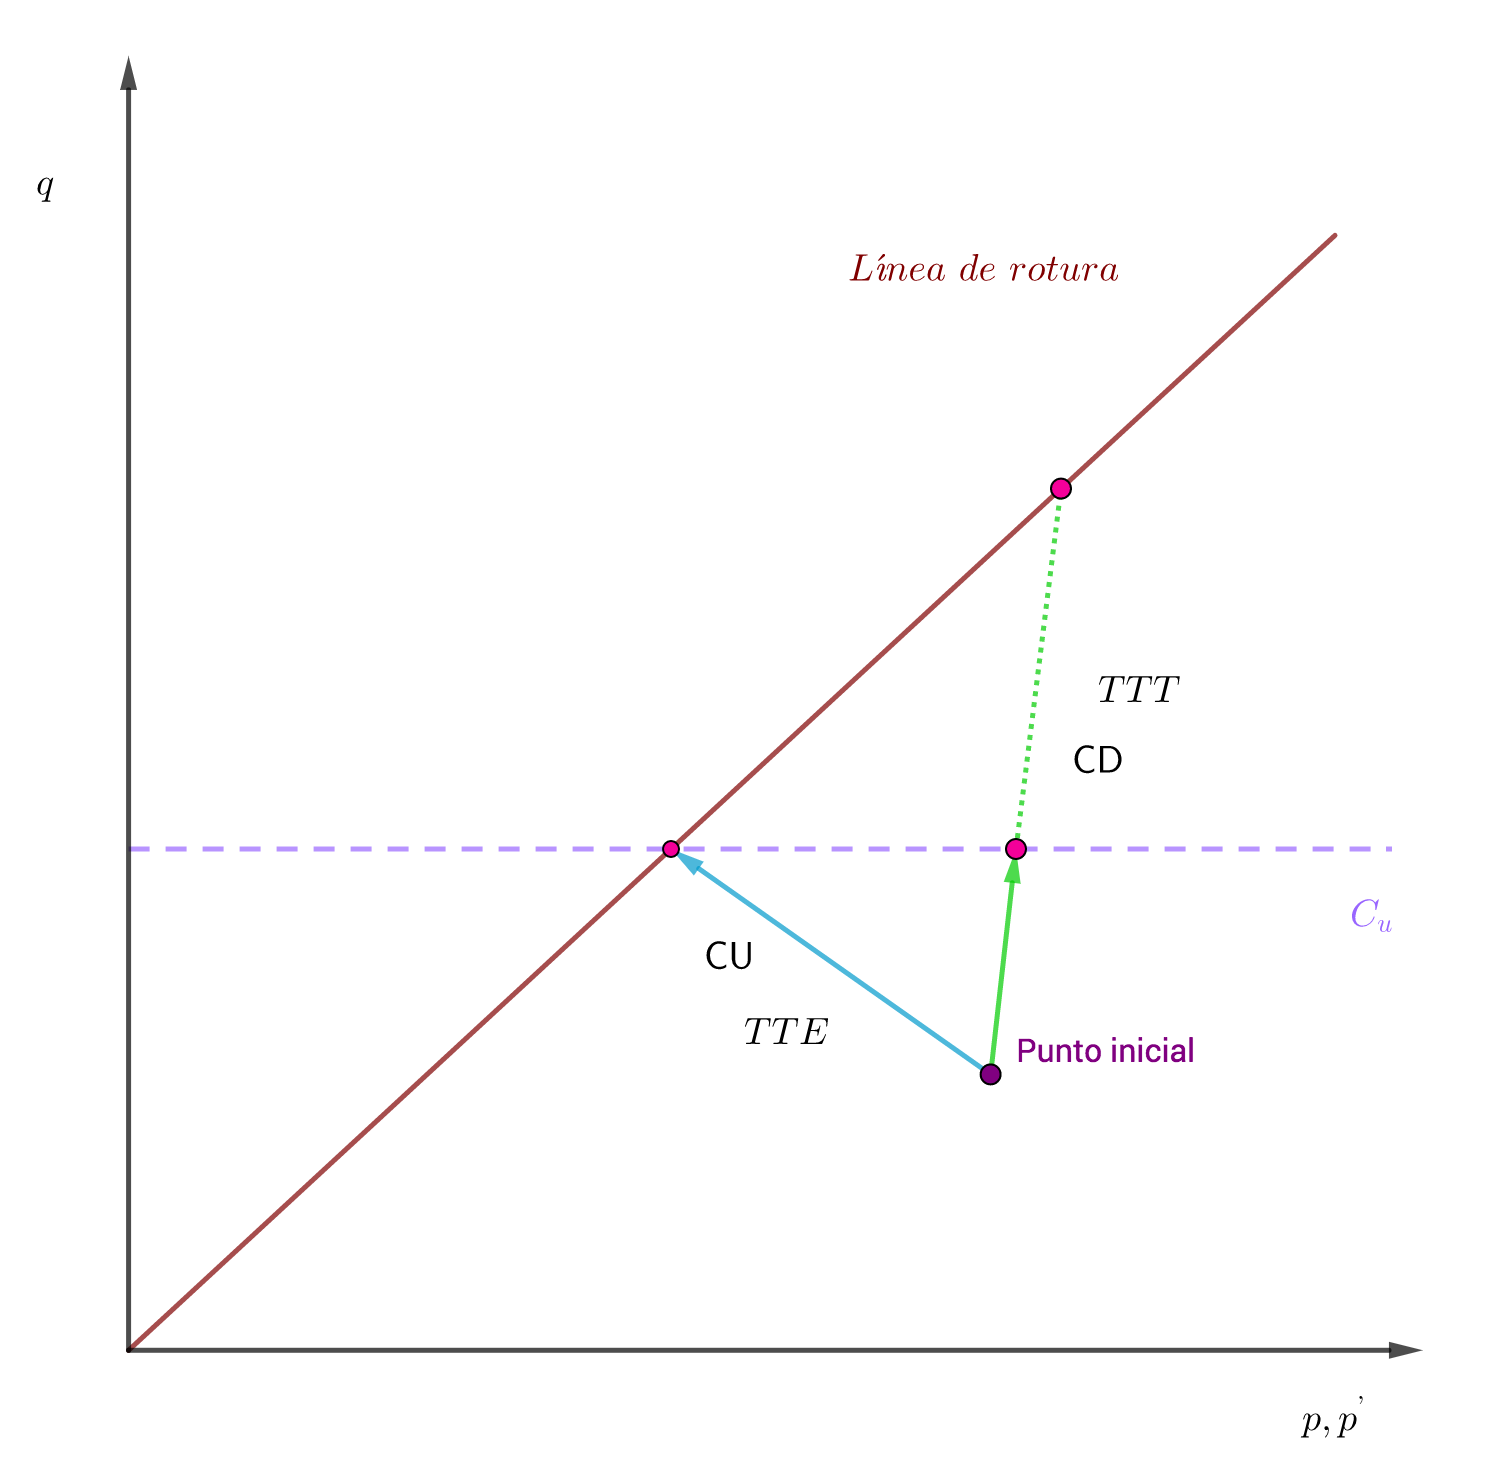
\includegraphics[width=0.5\textwidth]{img/trayectoria_tensiones}
		\caption{Trayectoria de tensiones }
		\label{fig:tensiones}
	\end{figure}
}

\question{Indica 3 posibles causas de deformación excesiva de una cimentación superficial no directamente relacionados con la carga aplicada}{
	\begin{enumerate}
		\item Levantamientos debidos a suelos expansivos o susceptibles a las heladas
		\item Deterioro del material de cimentación.
		\item Deformación por saturación de suelos colapsables (rellenos,loess)
		\item Deformación del terreno debido a excavaciones cercanas.
		\item Variación del NF
		\item Compactación del terreno por vibración, terremotos…
	\end{enumerate}
}

\question{La relación entre el asiento calculado por el método edométrico y por el método de Skempton es: 
\[
	S_{sb}= \mu S_{ed} = [A+\alpha (1-A)]S_{ed}
\]
Donde A es el parámetro de Skempton que depende de $\frac{z}{B}$. El valor de $\alpha$ para $\frac{z}{B}=0$ es 1. ¿Por qué?}{
	Una de las hipótesis del método edómetrico ($\epsilon_h = 0$) es que el incremento de presión intersticial es igual al incremento de presión vertical:
	\[
		\Delta u = \Delta \sigma_v
	\]
	El método de Skempton trata de mejorar esta aproximación introductiendo el parámetro $\mu = [A+\alpha (1-A)]$. Donde:
	\[
		\alpha \in[0,1] \propto 1-\frac{z}{B}
	\]
	En efecto si $\frac{z}{B}=0$, es decir la base es mucho mayor que la dimensión vertical del estrato (potencia), entonces nos situamos en condiciones edometricas y los asientos deben coincidir $\Rightarrow \alpha = 1$.
}


\question{Una placa de $\phi = 0,2m$ sometida a $10 T/m^2$ sufre un asiento de $0,2cm$. ¿Qué asiento se obtendrá al cargar una cimentación de $\phi = 1,2m$ y $20T/m^2$. Suponiendo suelo elástico-lineal?}{
	Tenemos $s \propto Q$ así pues:
	\[
		s_2 = s(2Q) = 2s(Q) = 2s_1
	\]
	Al tener un suelo elástico lineal $\frac{B}{s}=cte$, luego:
	\[
		s_3 = \frac{B_3}{B_2}s_2 
	\]	
	Luego mediante aplicación numerica $s_3 \approx 2,4cm$
}


\question{ En la práctica. ¿Esperarías que el asiento de la cimentación fuera mayor o menor que el calculado? ¿Por qué?}{
	La teoría elástico lineal no tiene en cuenta la variación del módulo elástico con la profundidad ($\frac{dE}{dz}>0$), luego es de esperar un asiento menor en la práctica.
}

\question{Las expresiones de la capacidad portante tienen la siguiente estructura (en terreno drenado):
\[
	q_r = cN_c + \frac{1}{2}\gamma B N_\gamma + qN_q
\]
}{
	\begin{enumerate}
	\item ¿A qué mecanismo de resistencia corresponde cada uno de los términos?
		\begin{enumerate}
			\item Contribución de la cohesión del suelo a la resistencia
			\item Efecto del peso
			\item Contribución de cargas sobre el plano de cimentación
		\end{enumerate}
	\item ¿Qué forma adopta en el caso de un terreno sumergido?
		En el caso de un terreno submergido hemos de tener en cuenta el efecto del empuje de Arquimedes, así pues podemos trabajar en tensiones efectivas:
		\begin{equation}
			\begin{cases}
				q_r^{’}=c^{’}N_c + \frac{1}{2}\gamma^{’} B N_\gamma + q^{’}N_q\\
				q_r =q_r^{’} + (p_w)_{base} 
			\end{cases}
		\end{equation}
	\item ¿Qué forma adopta en el caso de un análisis no drenado en tensiones totales $\phi = 0$
	Tenemos $N_q(\phi = 0)=1, N_\gamma(\phi = 0)=0$, luego:
	\[
		q_u = C_u N_c + q
	\]
	\item ¿Qué forma adoptaría q en el caso que el terreno de cimentación fuera exclusive agua?
	\begin{equation}
		\begin{cases}
			q_r =q_r^{’} + (p_w)_{base} = c^{’}N_c + \frac{1}{2}\gamma^{’} B N_\gamma + \gamma_w H_w, &\text{ drenado}\\
			q_r = C_uN_c + \gamma_w H_w,&\text{ no drenado}
		\end{cases}
	\end{equation}
\end{enumerate}
}

% section parte_2 (end)

\newpage

\section{Cimentaciones profundas} % (fold)
\label{sec:cimentaciones_profundas}

\begin{mybox}{Pilotes}
Es la máxima presión que puede sufrir el terreno bajo la cimentación
\tcbsubtitle{\emph{CPI 4}}
	\begin{enumerate}
		\item Avance tubería con cuchare o trépano
		\item Empotramiento del pilote
		\item Hormigonado y extracción de la tubería
	\end{enumerate}
\tcbsubtitle{\emph{CPI 7}}
	\begin{enumerate}
		\item Avance de la perforación con el auger
		\item Hormigonado
	\end{enumerate}
	\begin{myrem}[Restricción]
		El terreno ha de tener cierta cohesión
	\end{myrem}
\tcbsubtitle{\emph{CPI 8 (barrena continua)}}
	\begin{enumerate}
		\item Introducimos la barrena a rotación hasta el fondo (donde se quiere llegar)
		\item Se hormigona mientras se va quitando la barrena
		\item Introducción de la armadura en el hormigón fresco
	\end{enumerate}
	\begin{myrem}[Armaduras]
		Suelen trabajar a compresión, luego si la armadura no es más corta no tiene porque ser problemático.
	\end{myrem}
\tcbsubtitle{\emph{CPI 3 (hincado)}}
	\begin{enumerate}
		\item Hincado
		\item Formación del bulbo
		\item Hormigonado y extracción de la tuberia
	\end{enumerate}
\end{mybox}

\begin{figure}[H]
		\centering
		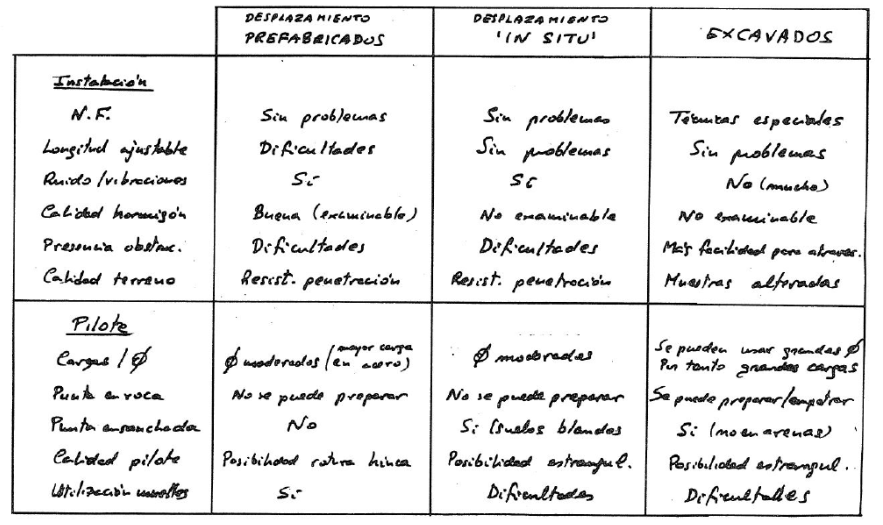
\includegraphics[width=\textwidth]{img/compar}
		\caption{Comparación de los distintos métodos}
		\label{fig:compar}
\end{figure}

\begin{mybox}{Método Delft}
	\begin{ldef}[Delft]
		Permite calcular la resistencia en punta de un pilote
	\end{ldef}

	La resistencia no es uniforme, así pues solemos estimar un único valor medio de la distribución.

	\tcbsubtitle{\emph{Procedimiento}}

	Se definen 3 zonas, de menor a mayor profundidad y se cálcula
	\begin{equation}
		\begin{cases}
			q_c = \frac{(q_c)_{I}+(q_c)_{II}}{2}, &\text{ if }(q_c)_{III} >(q_c)_{II} \\
			q_c = \frac{(q_c)_{I}+\frac{(q_c)_{II}+(q_c)_{III}}{2}}{2}, &\text{ if }(q_c)_{III} \leq(q_c)_{II}
		\end{cases}
	\end{equation}
\end{mybox}

% section cimentaciones_profundas (end)

\newpage



\section{Coeficiente de empuje} % (fold)
\label{sec:parte1}

\question{Explicar en pocas palabras 3 posibles métodos pasa calcular el empuje adicional causado por sobrecargas externas}{
	\begin{itemize}[label=\ding{69}]
		\item Uniforme:
		\begin{figure}[H]
			\centering
			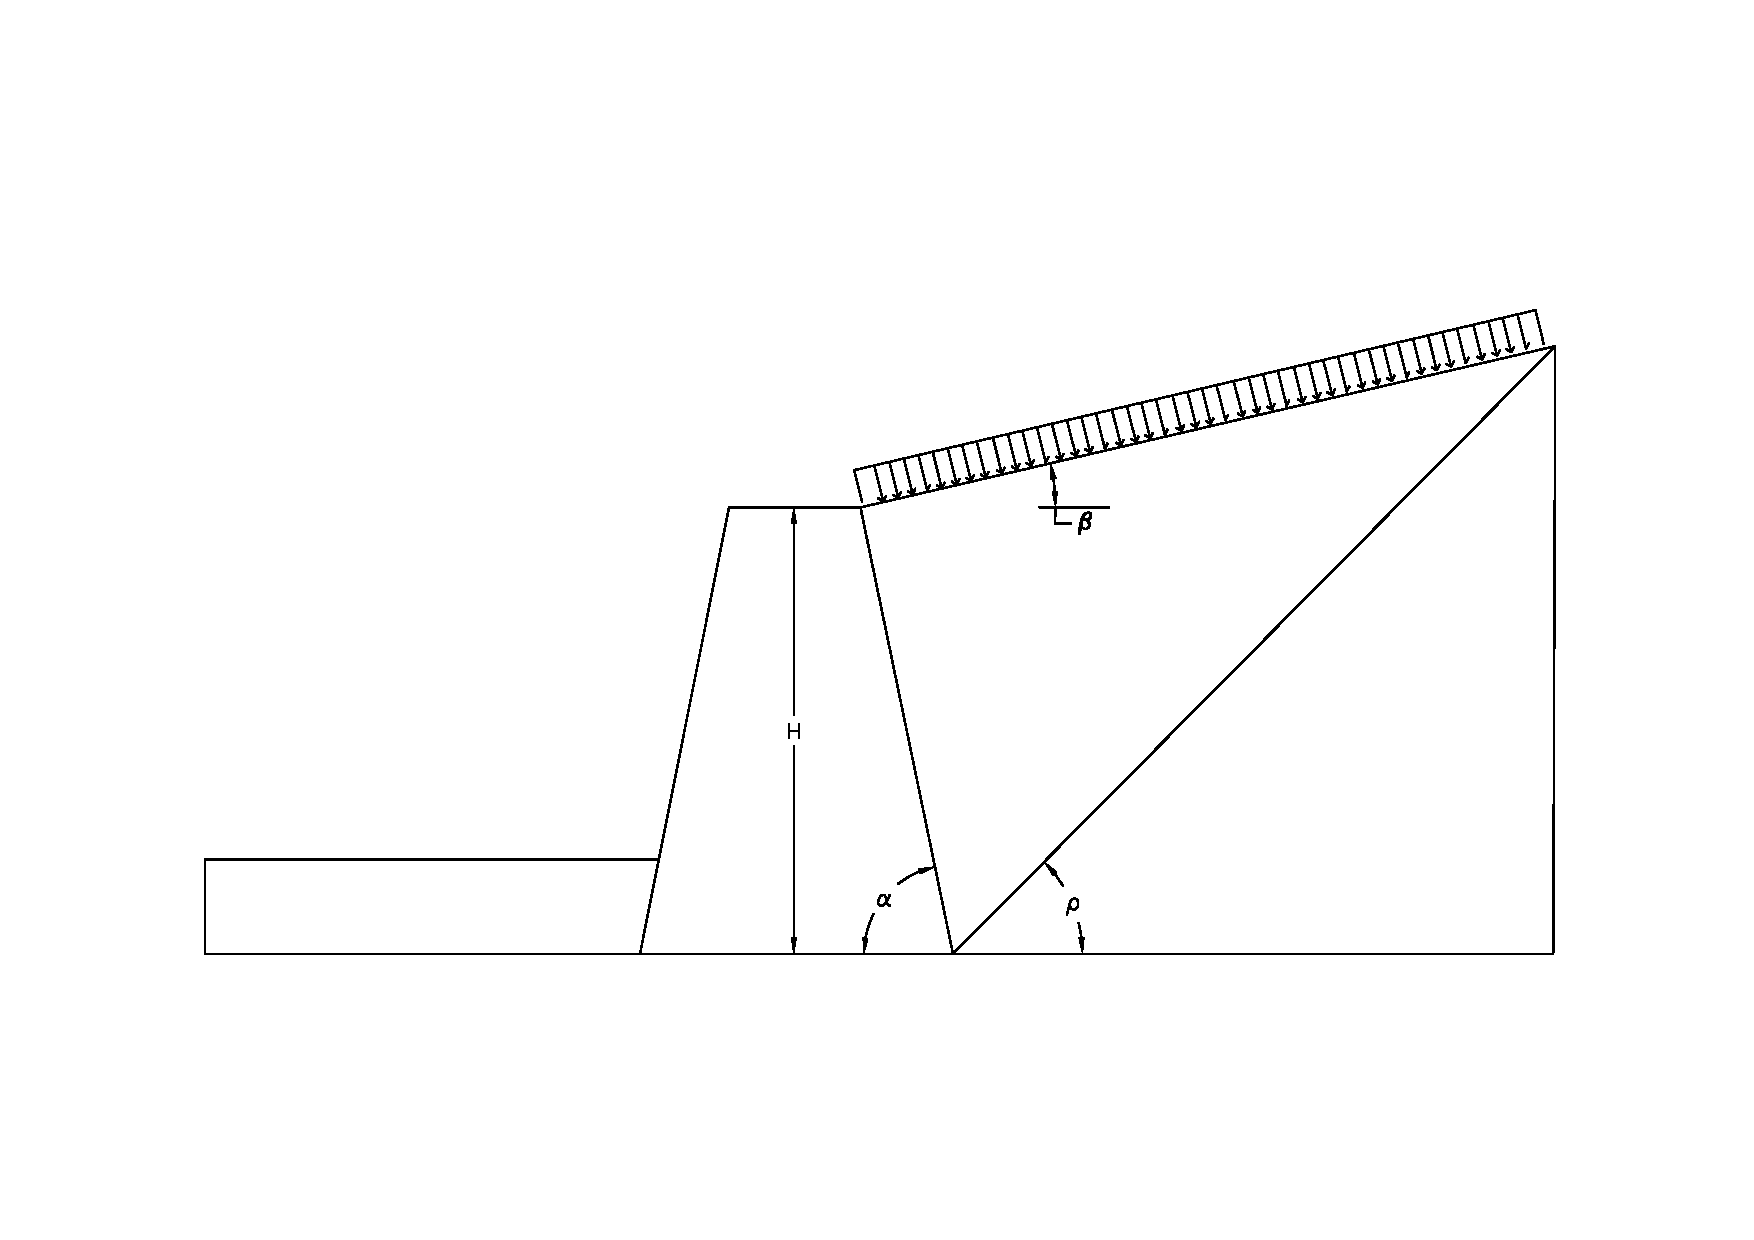
\includegraphics[width=0.7\textwidth]{img/cargas_uni}
			\caption{caption}
			\label{fig:Cargas uniformes}
		\end{figure}
		\[
			\gamma^{eq} = \gamma \frac{2q \sin(\alpha)}{H \sin(\alpha + \beta)}, \quad \emph{una densidad equivalente}
		\]
		O bien
		\[
			\Delta H = \frac{q \sin(\alpha)}{H \sin(\alpha+\beta)}, \quad \emph{una altura equivalente}
		\]
		\item No uniforme:
		\begin{figure}[H]
			\centering
			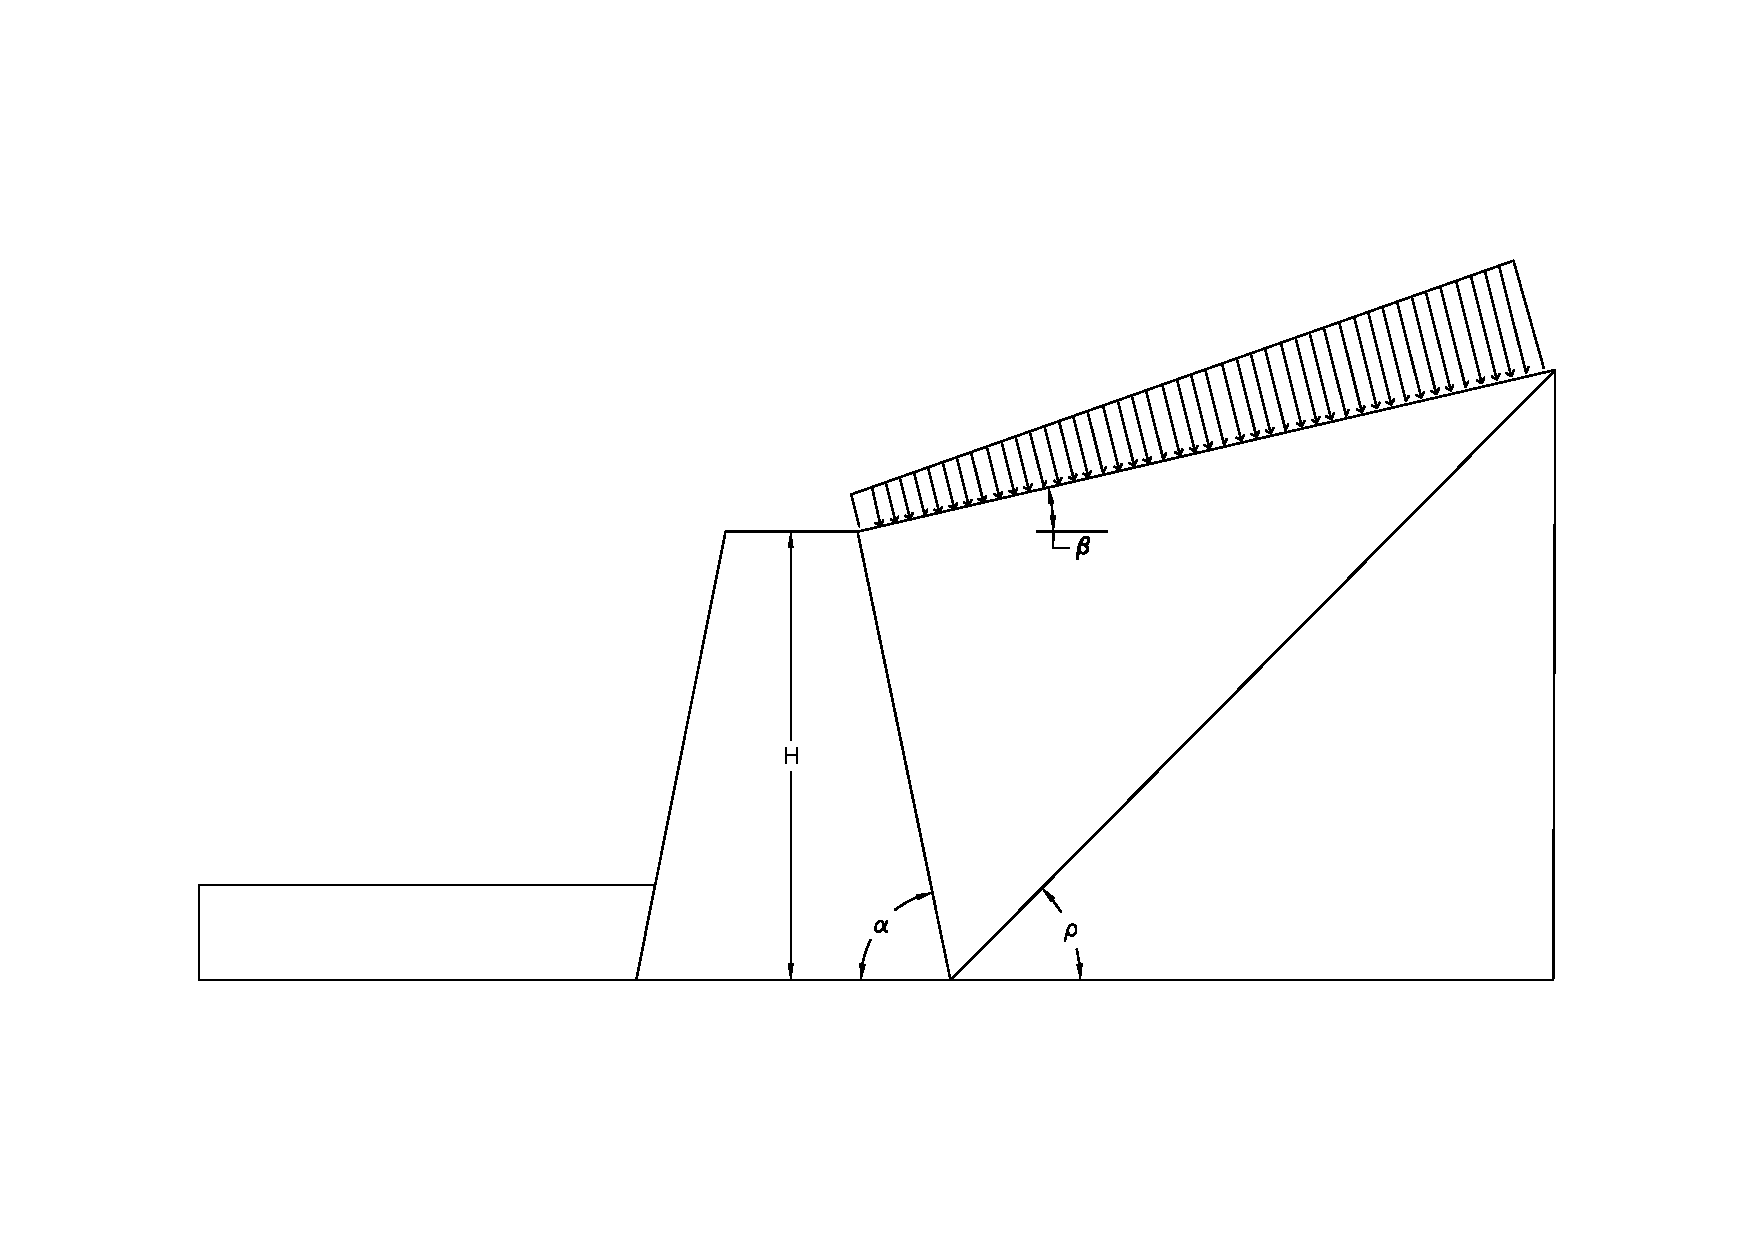
\includegraphics[width=0.7\textwidth]{img/cargas_no_uni}
			\caption{Cargas no uniformes}
			\label{fig:label}
		\end{figure}
		\begin{itemize}[label=\ding{71}]
			\item Soluciones elásticas (Boussinesq)
			\item Soluciones plásticas
			\item Reglas empíricas
		\end{itemize}
	\end{itemize}
}

\question{ Un muro con alto ángulo de rozamiento (40) está en contacto con un suelo de ángulo de fricción igual a 30. a) ¿ Qué valor escogerías como ángulo de rozamiento suelo-muro ? }{
	a)
	\[
		\delta = \frac{2}{3} \phi^{’}= 20
	\]
	b)
}

\question{¿ Qué diferencia conceptual existe entre el método de Coulomb y el de Rankine para el cálculo de empuje de tierras ? }{
	\begin{itemize}[label=\ding{69}]
		\item Rankine: 
		\begin{enumerate}
			\item no se considera rozamiento suelo-muro ($\delta=0$)
			\item se supone rotura completa del suelo
		\end{enumerate}
		\item Coulomb:
		\begin{enumerate}
			\item consideramos rozamiento suelo-muro ($\delta \neq 0$)
			\item Rotura según 2 planos, uno de ángulo $\rho$ y otro con el muro
		\end{enumerate}
	\end{itemize}
}

\question{Enumerar las razones por las que el metodo de Rankine es más seguro que el de Coulomb para el cálculo de empujes de tierras.}{
	\begin{enumerate}
		\item En el caso \textbf{pasivo} no es aconsejable usar Coulomb, pues sobre-estima lo que va a resistir el terreno 
		\[
			K_{pc}>K_{p-real} \Rightarrow E_{pc}>E{p-real}
		\]
		\item Rankine supone $\delta = 0 \Rightarrow$ \textbf{empuje activo máximo} ($\nexists$ componente estabilizadora del empuje) en la teoría de Coulomb supone parte del empuje como estabilizador 
		\[
		 	E_{Rankine} > E_{Coulomb}
		 \] 
		 \item Rankine supone rotura en todo el terreno, mientra Coulomb solo la considera en 2 lineas.
	\end{enumerate}
	Así pues el terreno rompe antes de lo que dica Coulomb.
}

\question{Cúal es la influencia de la fricción suelo-muro sobre: 
\begin{itemize}[label=\ding{69}]
	\item Empuje activo
	\item Empuje pasivo
	\item $K_0$
	\item Momento de vuelco por empuje activo
\end{itemize}}{
	\begin{itemize}[label=\ding{69}]
		\item \emph{Empuje activo:}
		\[
			\delta \approx \frac{2}{3} \phi^{’}
		\] 
		y 
		\[
			K_a = \frac{1- \sin(\phi^{’})}{1+ \sin(\phi^{’})} \Rightarrow \frac{\dif K_a}{\dif\phi^{’}}<0
		\]
		Con lo cual 
		\[
			\frac{\dif E_a}{\dif\delta}<0
		\]
		\item \emph{Empuje pasivo:}
		\[
			K_p = \frac{1+ \sin(\phi^{’})}{1+ \sin(\phi^{’})} \Rightarrow \frac{\dif K_a}{\dif\phi^{’}}>0
		\]
		Con lo cual 
		\[
			\frac{\dif E_p}{\dif\delta}>0
		\]
		\item $K_0$:
		No influye al estar en reposo
		\item \emph{Momento de vuelco por empuje activo}:
		\[
			\frac{\dif E_a}{\dif\delta}<0 \Rightarrow \frac{\dif M}{\dif\delta}<0
		\]
	\end{itemize}
}

\question{Dibujar cualitativamente la ley de empujes de Rankine sobre el muro de la Figure~\ref{fig:emp_gravedad}}{
	\begin{figure}[H]
		\centering
		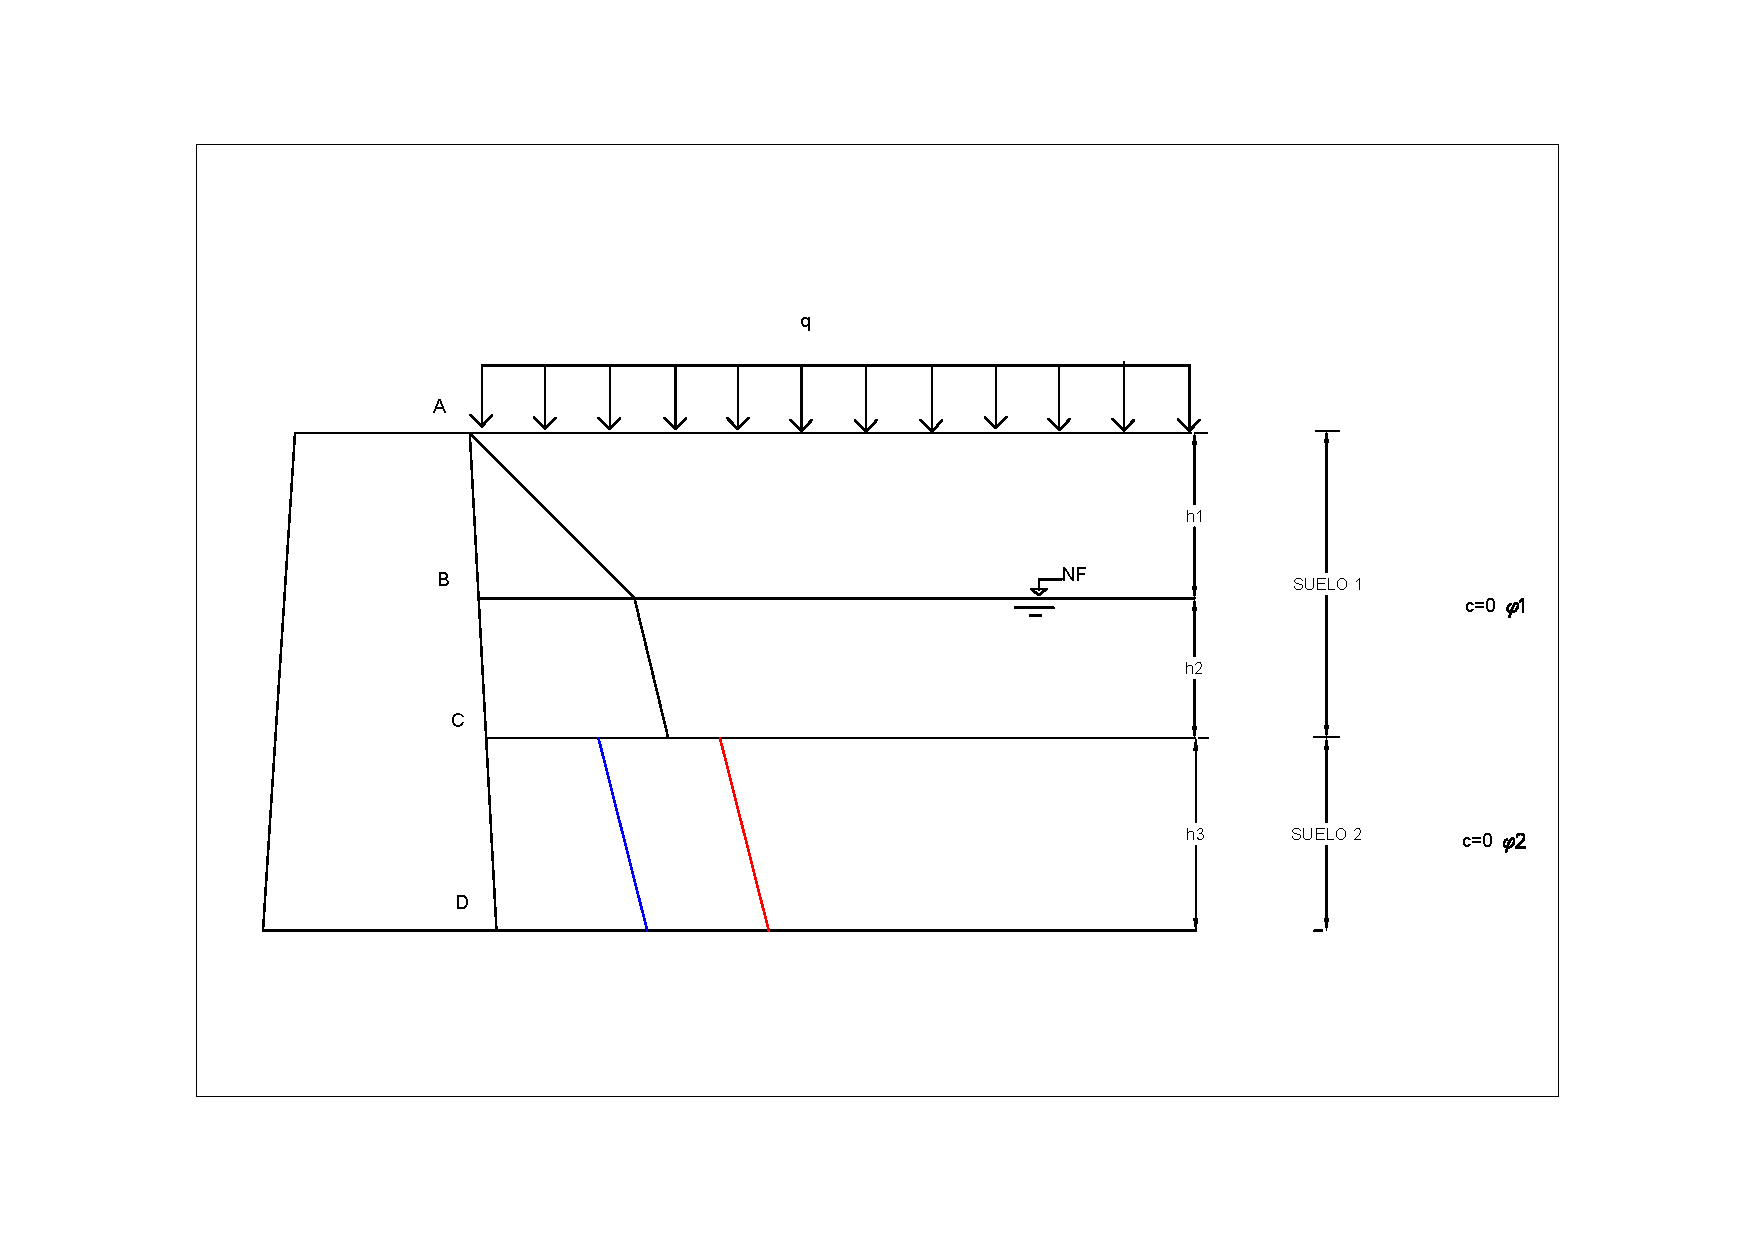
\includegraphics[width=0.9\textwidth]{img/ejemplo_empuje}
		\caption{Empuje de tierras sobre muro de gravedad}
		\label{fig:emp_gravedad}
	\end{figure}
	Tenemos:
	\begin{itemize}
		\item A: 
		\[
			\sigma_v^{’} = 0 \Rightarrow \sigma_h^{’}=0
		\]
		\item B:
		\[
			\sigma_v^{’} = \gamma h_1 + q \Rightarrow \sigma_h^{’}= K_a(\gamma h_1 + q)
		\]
		\item C:\\
		\emph{Parte superior:}
		\[
			\sigma_v^{’} = \gamma h_1 + \gamma^{’}h_2 + q \Rightarrow \sigma_h^{’}= K_a^{\phi_1}(\gamma h_1 + \gamma^{’}h_2+ + q)
		\]
		\emph{Parte inferior:}
		\[
			\sigma_v^{’} = \gamma h_1 + \gamma^{’}h_2 + q \Rightarrow \sigma_h^{’}= K_a^{\phi_2}(\gamma h_1 + \gamma^{’}h_2+ + q)
		\]
		\item D:
		\[
			\sigma_v^{’} = \gamma h_1 + \gamma^{’}(h_2+ h_3) + q \Rightarrow \sigma_h^{’}= K_a^{\phi_2}(\gamma h_1 + \gamma^{’}(h_2+ h_3) + q)
		\]

		\begin{myrem}
			En rojo el caso en el que $\phi_2 < \phi_1$ y en azul el contrario. En efecto tenemos $\frac{\dif K_a}{\dif\phi^{’}}>0$. Luego la variación de pendiente se debe a $\gamma^{’} < \gamma$
		\end{myrem}
	\end{itemize}
}

\question{Indicar qué parametros o propiedades fundamentales del terreno controlan el valor de $K_0$. ¿ Cómo varía $K_0$ con ellos ?}{

	EL grado de consolidación, $\phi^{’}$ y $I_p$. En el caso de tener una arcilla NC podemos considerar $K_0 = 1 - \sin(\phi^{’})$.

	\begin{minipage}{0.5\linewidth}
		\begin{figure}[H]
		\centering
		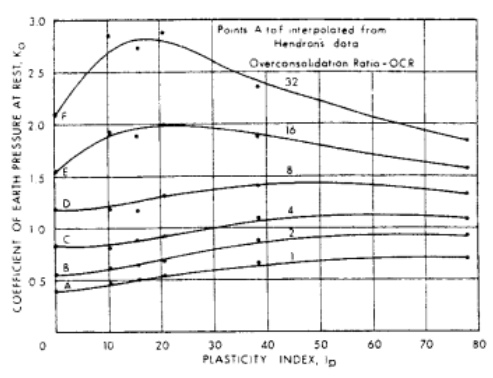
\includegraphics[width=\textwidth]{img/im1}
		\caption{caption}
		\label{fig:label}
		\end{figure}
	\end{minipage}%
	\begin{minipage}{0.5\linewidth}
		\begin{figure}[H]
			\centering
			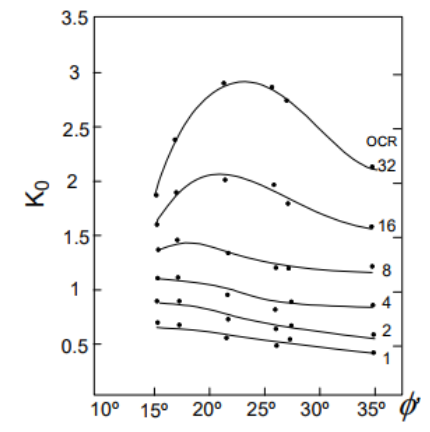
\includegraphics[width=\textwidth]{img/im3}
			\caption{caption}
			\label{fig:label}
		\end{figure}
	\end{minipage}
	
	\begin{figure}[H]
		\centering
		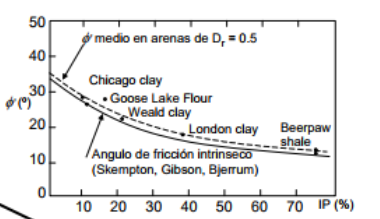
\includegraphics[width=0.5\textwidth]{img/im2}
		\caption{caption}
		\label{fig:label}
	\end{figure}
}

\question{¿ Cómo determinarías $K_0$ en laboratorio ? }{
	\begin{itemize}
		\item Ensayos edometricos
		\item Evaluación mediante succión (atención a la disminución de humedad)
	\end{itemize}
}

\question{ ¿ Podrías mencionar algún error conceptual que se admite en el desarollo del método del círculo de fricción para el cálculo del empuje pasivo ? Razonar para el caso c=0}{
	En el caso de empule pasivo en arcillas a largo plazo (c=0). Calcularemos el empuje pasivo como la suma de 2 estados:
	\begin{enumerate}
		\item Sólo interviene el peso sin cohesión $E_p^1$
		\item Sólo interviene la cohesión y el rozamiento del suelo, no interviene el peso $E_p^2$
	\end{enumerate}
	Luego $E_{total}=E_p^1+E_p^2$. Este procedimiento comporta errores:
	\begin{enumerate}
		\item Utilizo el método de estados límites de rotura $\rightarrow$ no se debe utilizar la superposición de estados.
		\item La superficie de rotura del estado 1 no tiene porque coincidir con la del estado 2.
	\end{enumerate}
	Estos errores se compensan ya que este metodo da resultados aceptables.
}

\question{ ¿ Están del lado de la seguridad los empujes pasivos alcanzados según Coulomb ?}{
	No, ya que sobre-estiman el empuje del suelo (al tener en cuenta el rozamiento).
}

\question{ ¿ Para movilizar $K_a$ son necesarias mayores $\varepsilon$ que para $K_p$ ?}{
	No, es al revés.
	\begin{figure}[H]
		\centering
		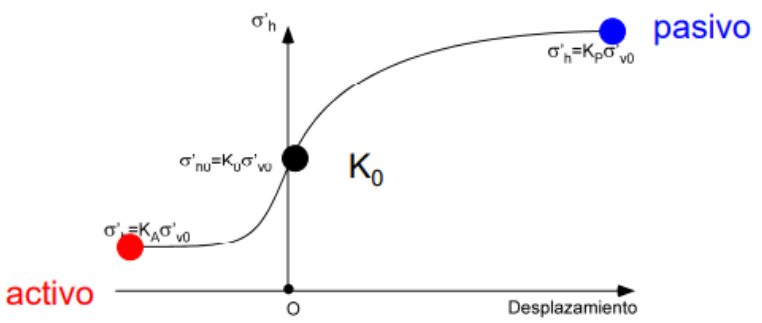
\includegraphics[width=0.5\textwidth]{img/im4}
		\caption{caption}
		\label{fig:label}
	\end{figure}

}

\question{¿ Puede darse el caso de que Coulomb prediga unas condiciones más desfavorables que Rankine en el caso activo ?}{
	No, ya que al considerar el rozamiento parte del empuje es estabilizador.
}

\question{ Hipótesis y utilización de la fórmula de Rankine }{
	\begin{enumerate}
		\item Todo el suelo esta en rotura
		\item La superficie de rotura es plana
		\item Rozamiento suelo/muro es nulo $\Rightarrow$ Tensiones principales
	\end{enumerate}
	Uso:
	\begin{enumerate}
		\item Trasdós vertical
		\item Terreno horizontal o inclinado un ángulo $\beta$
	\end{enumerate}
}

\question{Hipótesis de Coulomb para la determinación del empuje activo}{
	\begin{enumerate}
		\item Rotura plana: las lineas de contorno están en rotura 
		\item ``Suelo no cohesivo (c’=0) $\rightarrow$ friccional''
		\item ``No existen cargas aplicadas en superficie''
		\item Suelo homogéneo
		\item Suelo isotropo
		\item ``No hay agua $\rightarrow$ suelo seco''
	\end{enumerate}
}

\question{ En que casos se puede utilizar la teoría de Coulomb para la determinación del empuje pasivo ? Razonar}{
	Coulomb sobre-valora el empuje pasivo al considerar el rozamiento. Supone roturas planas cuando en realidad son curvas. Cúanto mayor sea $\delta$ mayor la distancia con la realidad.
}


% section questions (end)

\newpage

\section{Estructuras de contención} % (fold)
\label{sec:estructuras_de_contención}

\subsection{Muros de gravedad} % (fold)
\label{sub:muros_de_gravedad}

\begin{mydef}[Regla del núcleo central]
	Corresponde a la condición de no existencia de tracciones (suponiendo una distribución lineal). No es restristictiva se puede prescindir de ella en casos de terrenos duros (arcillas duras, rocas…). Ocurre si el punto de aplicación de la resultante respecto la base es :
	\[
		e> \frac{B}{6}
	\]
\end{mydef}


\subsection{Pantallas} % (fold)
\label{sub:pantallas}

\begin{mybox}{Pantallas}
	Son estructuras esbeltas, construidas con material que resiste a la tracción (acero, hormigón armado)
	\tcbsubtitle{\emph{Tablestacas}}

	\begin{minipage}[t]{0.5\textwidth}
	Ventajas:
	\begin{enumerate}
		\item Flexibles
		\item Estancas
		\item Reutilización fácil
	\end{enumerate}
	\end{minipage}%
	\begin{minipage}[t]{0.5\textwidth}
	Inconvenientes:
		\begin{itemize}
			\item Limitación de longitud
			\item Corrosión
			\item Difíciles de soldar
			\item No se pueden instalar en cualquier terreno
		\end{itemize}
	\end{minipage}

	\tcbsubtitle{\emph{Hormigonadas ``in-situ''}}
	Problemas comunes:
	\begin{itemize}
		\item Fallos de hormigonado (mala colocación)
		\item Fallos de inyección (falta adherencia)
		\item Mala calidad de los materiales
	\end{itemize}

	\tcbsubtitle{\emph{Otros tipos de pantallas}}
	\begin{itemize}
		\item Pilotes
		\item Micro-pilotes
		\item Damas
		\item Entibaciones
	\end{itemize}

	\tcbsubtitle{\emph{Posibles modos de fallo}}

	\tcbsubtitle{\emph{Estado tensional en voladizo}}

	\begin{minipage}[t]{0.5\textwidth}
	\begin{figure}[H]
		\centering
		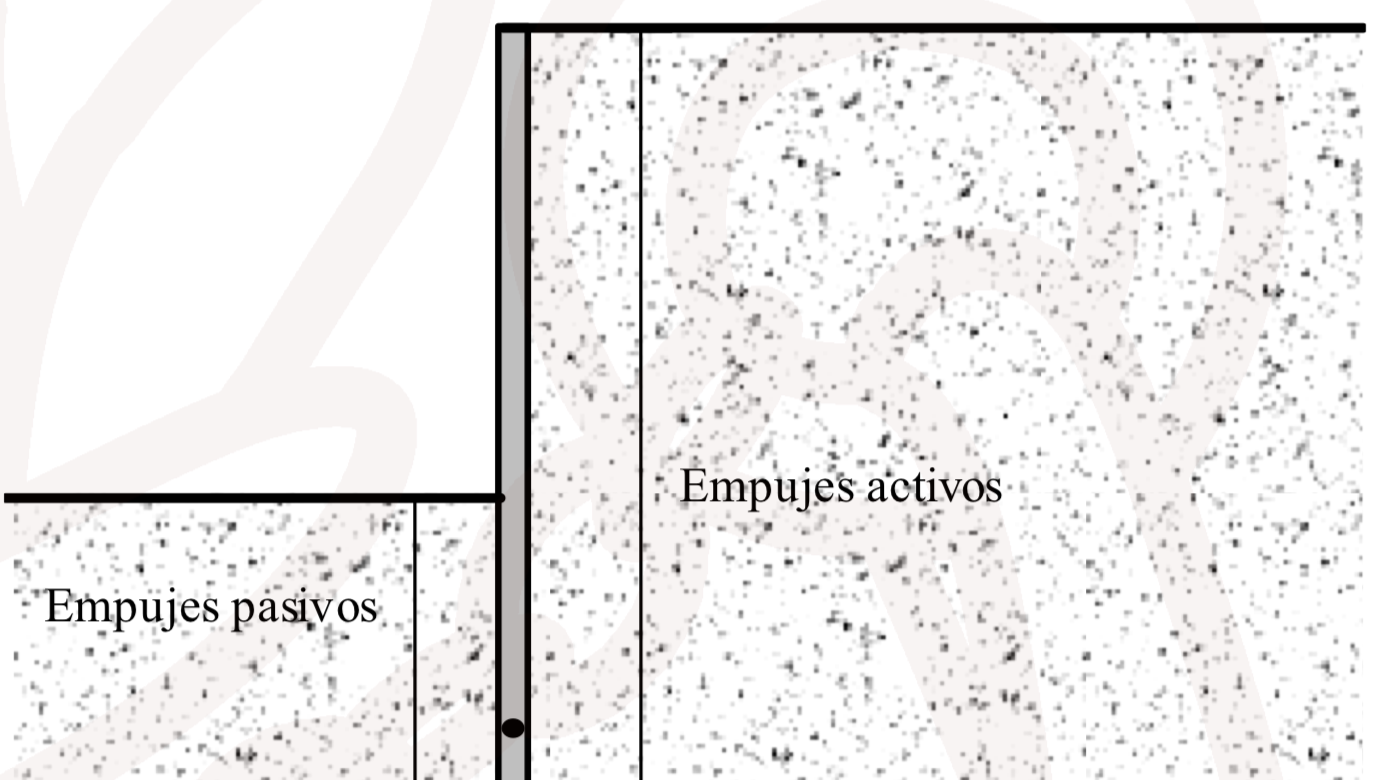
\includegraphics[width=0.95\textwidth]{img/confi1}
		\caption{Estado tensional 1 (translación)}
		\label{fig:confi1}
	\end{figure}
	\end{minipage}%
	\begin{minipage}[t]{0.5\textwidth}
	\begin{figure}[H]
		\centering
		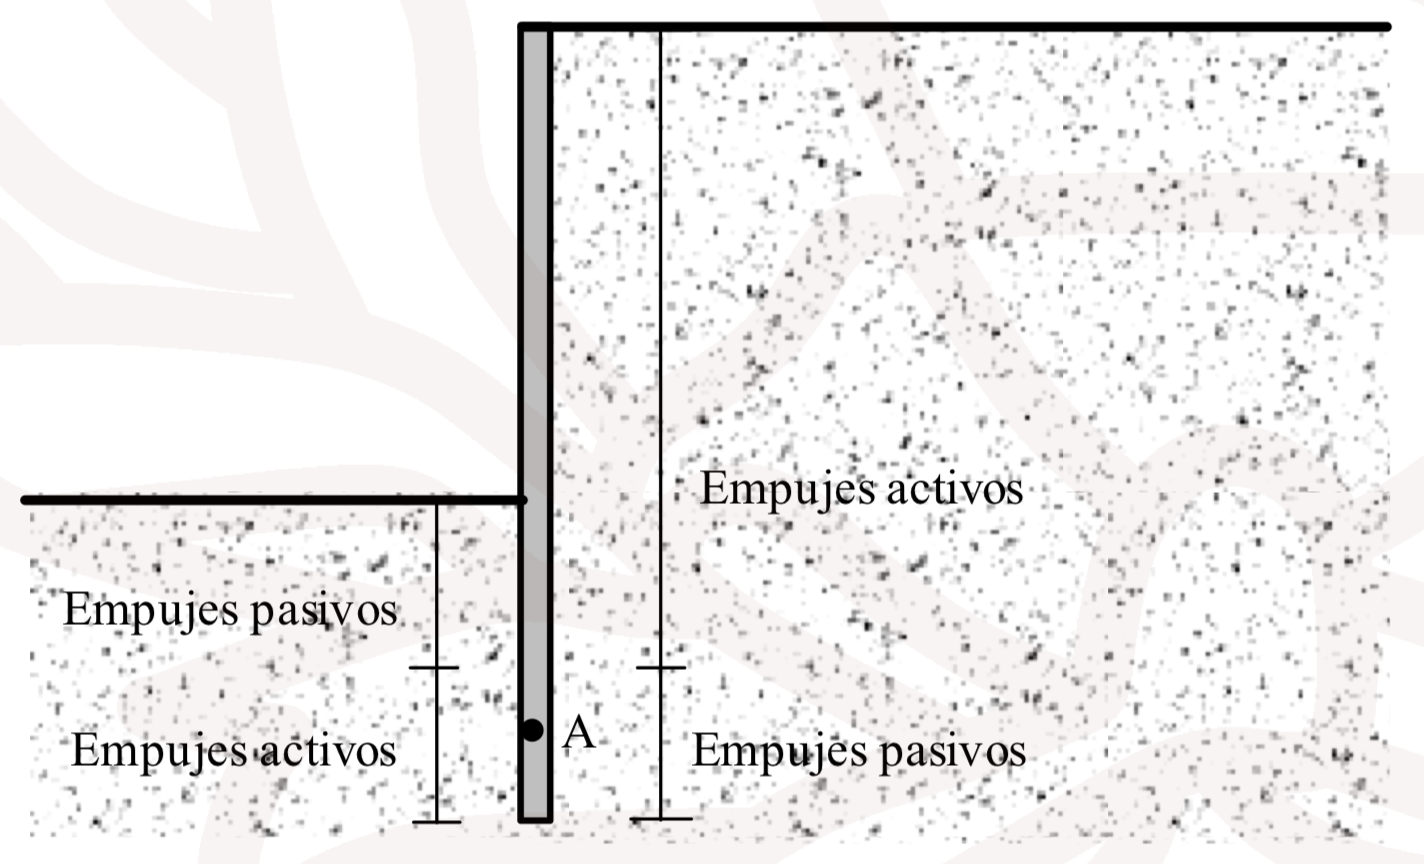
\includegraphics[width=0.95\textwidth]{img/confi2}
		\caption{Estado tensional 2 (rotación)}
		\label{fig:confi2}
	\end{figure}
	\end{minipage}

	\tcbsubtitle{\emph{Métodos de análisis}}

	\paragraph{En voladizo} % (fold)
	\label{par:en_voladizo}

	Sólo podemos analizar el caso de la Figure~\ref{fig:confi2} ya que la Figure~\ref{fig:confi1} no es estable.
	
	\begin{figure}[H]
		\centering
		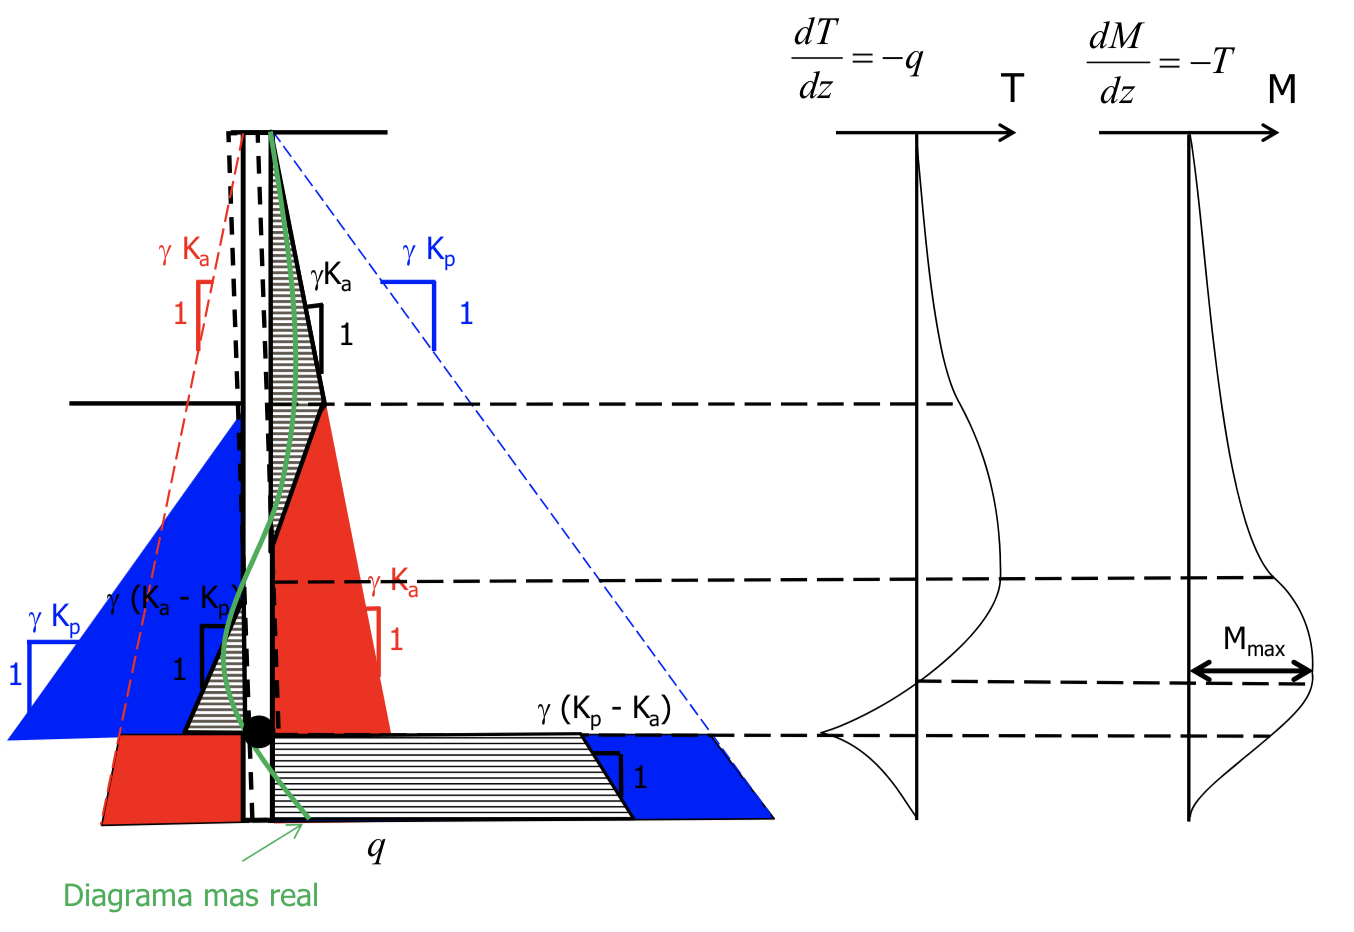
\includegraphics[width=0.95\textwidth]{img/voladizo}
		\caption{Análisis voladizo}
		\label{fig:voladizo}
	\end{figure}
	% paragraph en_voladizo (end)

	\paragraph{Soporte libre} % (fold)
	\label{par:soporte_libre}
	El estado tensional es cómo Figure~\ref{fig:confi1}. Este método considera que la profundidad del empotramiento es pequeña o que la rigidez de la pantalla es grande. Se asume que la pantalla se desplaza de una manera rígida bajo el efecto de la \emph{presión activa} de tierras y moviliza la presión pasiva a lo largo de su parte empotrada. Se considera que no hay reacción en la base. Es un sistema isostático no necesitamos hipótesis adicionales.
	\begin{figure}[H]
		\centering
		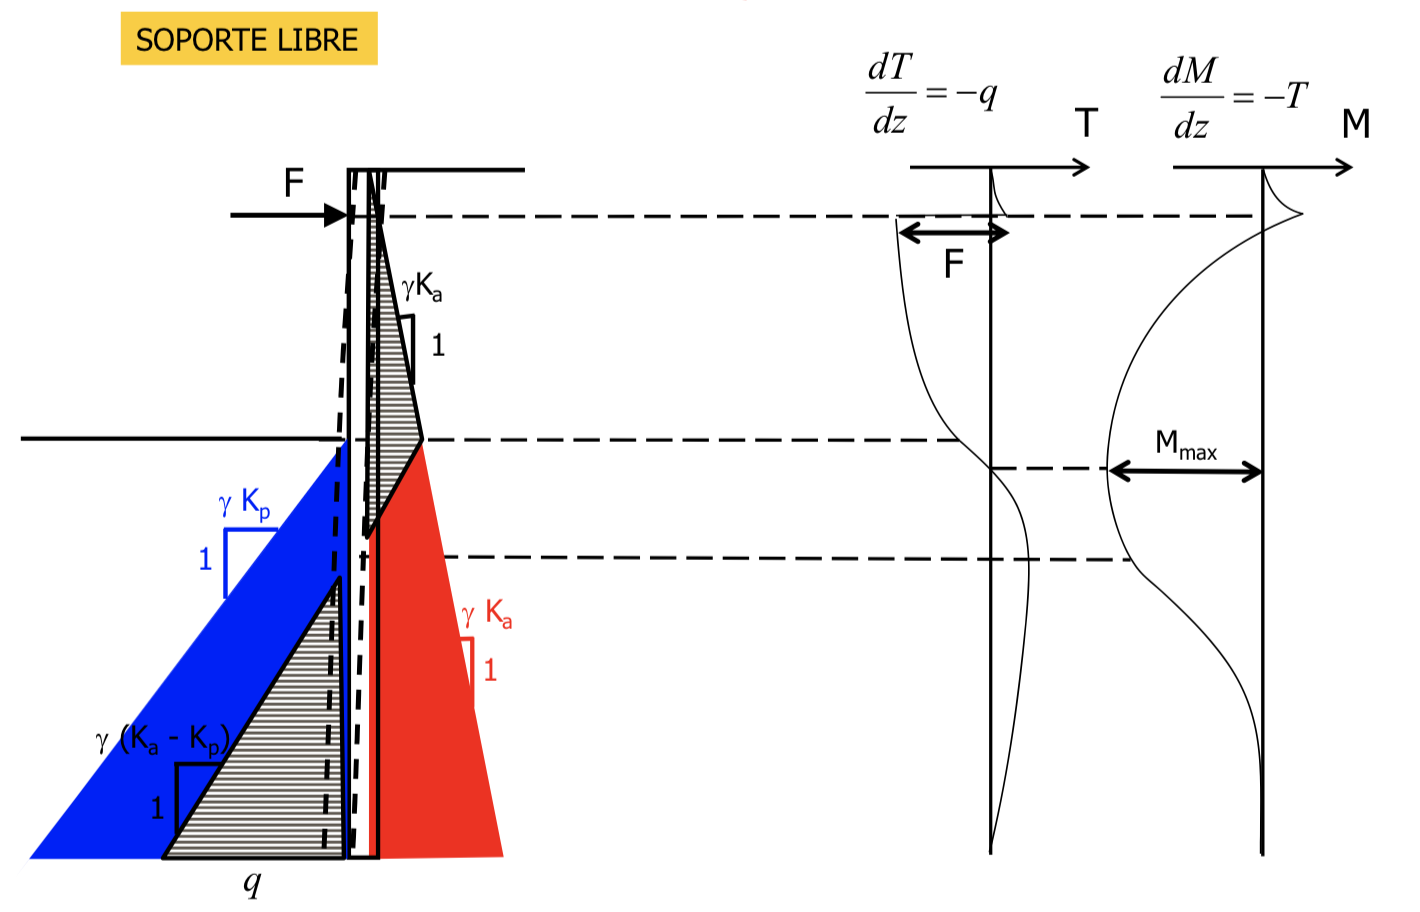
\includegraphics[width=0.95\textwidth]{img/soporte_libre}
		\caption{Análisis soporte libre}
		\label{fig:soporte_libre}
	\end{figure}
	% paragraph soporte_libre (end)

	\paragraph{Soporte fijo} % (fold)
	\label{par:soporte_fijo}
	El estado tensional es cómo la Figure~\ref{fig:confi2}. Este método considera que la rigidez es pequeña o la profundidad del empotramiento grande. Se considera que la base está empotrada. Este sistema es hiperestático, así pues es necesario realizar la hipótesis siguiente para resolverlo.
	\[
		x | \ q=0 \Leftrightarrow T(x) = T_{max} := M(x)=0
	\]
	\begin{figure}[H]
		\centering
		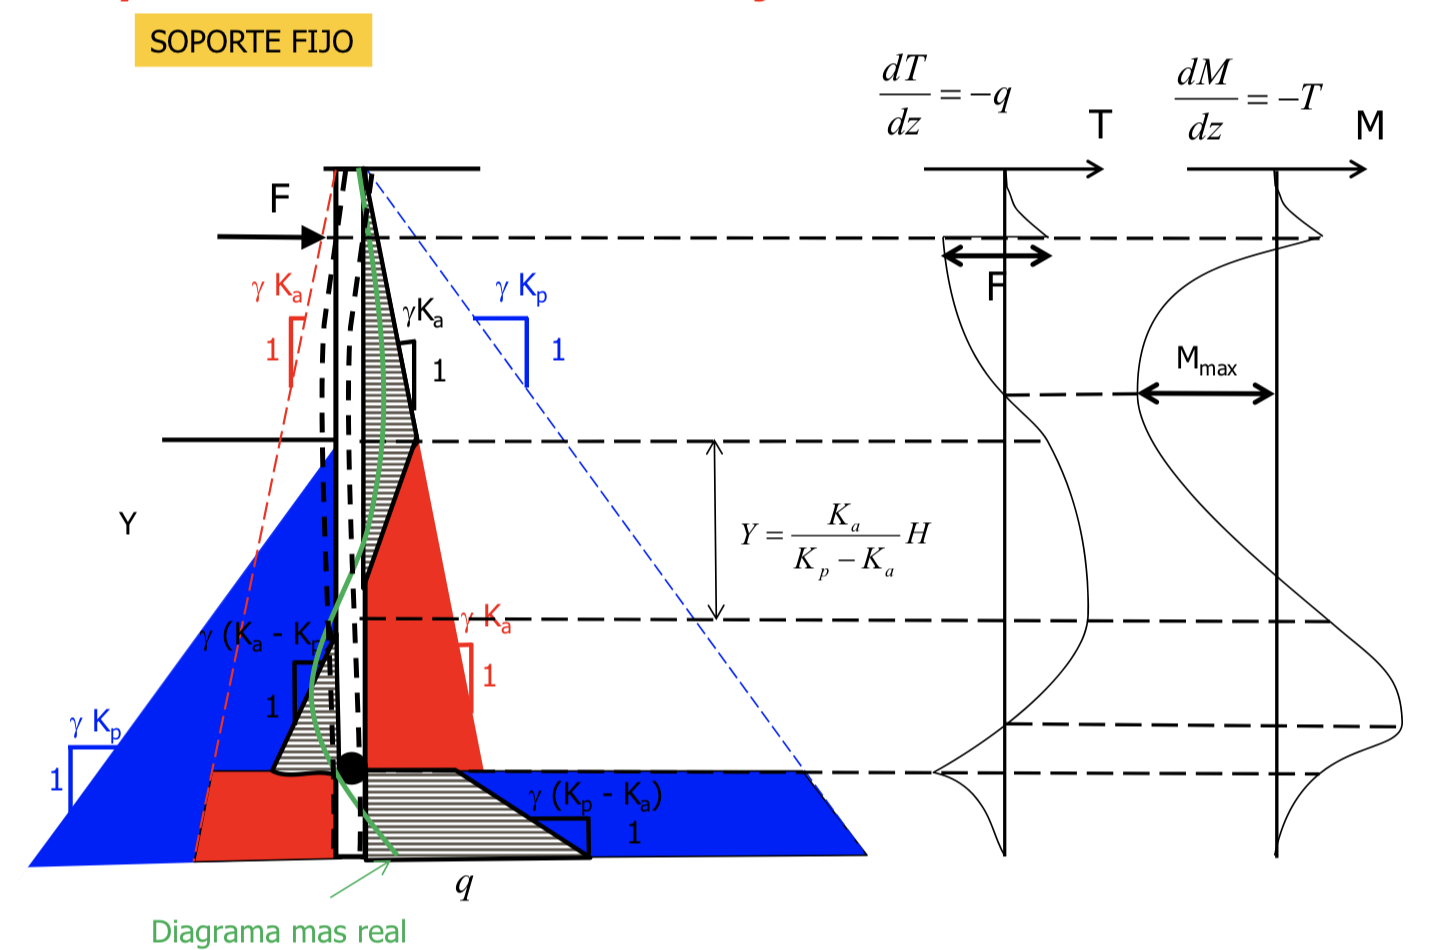
\includegraphics[width=0.95\textwidth]{img/soporte_fijo}
		\caption{Análisis soporte fijo}
		\label{fig:soporte_fijo}
	\end{figure}
	% paragraph soporte_fijo (end)
\end{mybox}

\begin{mybox}{Tierra reforzada}
	No requieren cimentación, tienen un buen comportamiento en suelos de mala calidad y permiten alturas importantes ($h>20m$)
	\begin{minipage}[t]{0.5\textwidth}
	Ventajas:
	\begin{enumerate}
		\item Estructura flexible (se adapta a asientos importantes en cimentación)
		\item Ejecución rápida con material ligero
		\item Coste competitivo
		\item Se pueden alcanzar alturas importantes
	\end{enumerate}
	\end{minipage}%
	\begin{minipage}[t]{0.5\textwidth}
	Inconvenientes:
		\begin{itemize}
			\item Relleno debe ser de calidad
			\item Problemas de durabilidad (corrosión de armaduras)
		\end{itemize}
	\end{minipage}
	\tcbsubtitle{\emph{Posibles modos de fallo}}

	\begin{enumerate}
		\item Por rotura a tracción de la armadura
		\item Por falta de adherencia armadura-relleno en la zona resistente
	\end{enumerate}

	\tcbsubtitle{\emph{Condiciones de estabilidad}}
	\begin{enumerate}
		\item Rotura a tracción:
		\[
			T_M \leq \frac{1}{F_1}\sigma_r b e
		\]
		\item Adherencia:
		\[
			T_M^{*}\leq \frac{1}{F_2}\int_0^{2a}\mu^* \sigma_v(x)2bdx
		\]

	\end{enumerate}
	Cálculo de la tracción máxima:
	\[
		T_M = \frac{1}{n}\sigma_h \Delta H
	\]
\end{mybox}

% subsection pantallas (end)
% subsection muros_de_gravedad (end)
% section estructuras_de_contención (end)

\newpage

\addcontentsline{toc}{section}{Bibliografia}
\nocite{*}
\printbibliography

\end{document}